\documentclass[12pt]{article}

\usepackage[utf8]{inputenc}
\usepackage[T1]{fontenc}
\usepackage{microtype}
\usepackage[brazil]{babel}
\usepackage{csquotes}
\usepackage[sortcites=true, backend=biber]{biblatex} 
\usepackage{bm}
\usepackage{times}
\usepackage{amsfonts}
\usepackage{amsmath}
\usepackage{amsthm}
\usepackage{graphicx}
\usepackage{indentfirst}
\usepackage{float}
\usepackage{hyperref}
\usepackage{booktabs}
\usepackage{caption}
\usepackage{algorithm}
\usepackage{algpseudocode}
\usepackage{multirow}
\usepackage{enumitem}
\usepackage[left=3cm, right=1.5cm, top=3cm, bottom=2cm]{geometry}
\usepackage{setspace}
\onehalfspacing

\newtheorem{observation}{Observação}
\newtheorem{definition}{Definição}
\newtheorem{proposition}{Proposição}
\newtheorem{example}{Exemplo}
\DeclareMathOperator{\prox}{prox}
\DeclareMathOperator*{\argmin}{arg\ min}
\newcommand{\norm}[1]{\left\lVert#1\right\rVert}

\addbibresource{referencias.bib}

\title{Influência do Uso de Busca Linear Exata na Convergência de Métodos Acelerados de Gradiente Proximal}
\author{Orientador: Elias Salomão Helou Neto\\Aluno: Gabriel Ligabô Baba}

\begin{document}
\begin{titlepage}
    \begin{center}
        {\large \sc UNIVERSIDADE DE SÃO PAULO} \\
        {\large \sc INSTITUTO DE CIÊNCIAS MATEMÁTICAS E DE COMPUTAÇÃO}\\[0.7cm]
        {\small \sc DEPARTAMENTO DE MATEMÁTICA APLICADA E ESTATÍSTICA}
        
        \vspace{4cm}
        
        {\large \sc Relatório Científico Final}\\
        \rule{\linewidth}{2pt}
        
        \vspace{0.7em}
        {\Large \bfseries Influência do Uso de Busca Linear Exata na Convergência de Métodos Acelerados de Gradiente Proximal}
        \vspace{0.2em}
        
        \rule{\linewidth}{2pt} \\
        {\small \sc Linha de Fomento: Bolsa no País - Regular - Iniciação Científica}
    \end{center}
    
    \vspace{1.8cm}
    
    \begin{flushleft}
        \textbf{Processo FAPESP}: 2025/12023-2\\
        \textbf{Período de vigência}: 01/09/2025 a 31/08/2026\\
    \end{flushleft}
    
    \vspace{1.8cm}
    
    \begin{minipage}{0.43\textwidth}
        \emph{Bolsista:}\\
        Gabriel Ligabô Baba
    \end{minipage}
    \hspace{1cm}
    \begin{minipage}{0.43\textwidth}
        \emph{Orientador:}\\
        Elias Salomão Helou Neto    
    \end{minipage}
    
    \vfill
    
    \begin{center}
        São Carlos -- SP \\
        Agosto de 2026
    \end{center}
\end{titlepage}

\setcounter{page}{2}
\newpage
\tableofcontents
\vspace{1cm} 

\begin{abstract}
Neste trabalho investigou-se o impacto da busca linear exata em métodos de otimização suave e de gradiente proximal (ISTA/FISTA) para reconstrução de imagens. Em problemas quadráticos, a busca exata acelera a convergência de métodos como o Nesterov, mas em problemas regularizados com termos não suaves (norma $\ell_1$ no domínio \textit{wavelet} e regularização por variação total) os passos calculados ignoram a geometria do termo de regularização, causando instabilidade assintótica. Observou-se, porém, um fenômeno consistente de semi-convergência, onde o FISTA com o passo exato atinge rapidamente uma alta qualidade de reconstrução. Os resultados sugerem que estratégias híbridas de otimização podem ser promissoras.
\end{abstract}

\section{Introdução}

A reconstrução de imagens em tomografia computadorizada (TC) configura um problema inverso tipicamente mal condicionado. Para obter soluções estáveis e mitigar os ruídos inerentes à amostragem da transformada de Radon, o problema é formulado matematicamente com a adição de termos de regularização convexos, porém frequentemente não diferenciáveis, como a variação total (TV) ou a norma $\ell_1$ no domínio \textit{wavelet}. Essa característica exige o emprego de algoritmos de gradiente proximal, destacando-se o FISTA (\textit{Fast Iterative Shrinkage-Thresholding Algorithm}) por sua aceleração via \textit{momentum} de Nesterov.

A eficiência de tais métodos de primeira ordem é dependente da escolha do tamanho de passo. Abordagens clássicas utilizam um passo fixo (limitado pelo inverso da constante de Lipschitz do operador suave) ou buscas inexatas adaptativas, como o \textit{backtracking}. No entanto, em aplicações de larga escala como a TC, o cálculo exato da constante de Lipschitz não possui fórmula analítica fechada e sua aproximação numérica pode ser custosa, enquanto a busca inexata por \textit{backtracking} diminui a eficiência computacional devido às repetidas avaliações do operador de projeção.

Como a parcela suave continua sendo quadrática, surge a hipótese de que um passo calculado exclusivamente para essa parcela possa acelerar a convergência dos métodos proximais. Com isso, este projeto investiga a utilização de uma busca linear exata, calculada analiticamente de forma relativamente barata, considerando apenas a parcela quadrática da função objetivo. Especificamente, este trabalho tem como objetivos: (i) avaliar a busca exata em problemas quadráticos irrestritos, comparando-a às estratégias de passo fixo, \textit{backtracking} e ao método dos gradientes conjugados; (ii) otimizar algebricamente seu cálculo em tomografia computadorizada; (iii) analisar a eficácia dessa forma de calcular o tamanho de passo em problemas regularizados por normas não suaves ($\ell_1$ \textit{wavelet} e variação total); e (iv) avaliar o comportamento dos algoritmos, ponderando se a eliminação do custo iterativo do \textit{backtracking} compensa os eventuais impactos na estabilidade e convergência do método.

\subsection{ISTA e FISTA}
\label{problema}
Quando estamos lidando com o problema compósito:
\[
\min_{\mathbf{x}} F(\mathbf{x}) = f(\mathbf{x}) + \gamma g(\mathbf{x})
\]
onde $f(\mathbf{x})$ é uma função suave e convexa e $g(\mathbf{x})$ é uma função convexa não suave, uma possível forma de resolvê-lo é utilizando o método ISTA (\textit{Iterative Shrinkage-Thresholding Algorithm}). A ideia por trás deste método é aproveitar a suavidade de $f$ para realizar um passo do gradiente e, em seguida, corrigir o efeito da parte não diferenciável via operador proximal:

\begin{algorithm}[H]
\caption{ISTA}
\begin{algorithmic}[1]
\State \textbf{Entrada:} $\mathbf{x_0} \in \mathbb{R}^n$, $\lambda > 0$.
\For{$k = 0, 1, 2, \dots$}
    \State $\mathbf{x_{k+1}} = \operatorname{prox}_{\gamma \lambda g} ( \mathbf{x_k} - \lambda \nabla f( \mathbf{x_k} ) )$
\EndFor
\State \textbf{Retorno:} Solução aproximada $\mathbf{x^*}$.
\end{algorithmic}
\end{algorithm}

Uma variação mais eficiente desse algoritmo é o FISTA (\textit{Fast Iterative Shrinkage-Thresholding Algorithm}) \cite{bet09}, que utiliza o \textit{momentum} de Nesterov para acelerar a convergência:

\begin{algorithm}[H]
\caption{FISTA}
\begin{algorithmic}[1]
\State \textbf{Entrada:} $\mathbf{x_0} \in \mathbb{R}^n$, $\lambda > 0$.
\State \textbf{Inicialização:} $\mathbf{y_1} = \mathbf{x_0}$, $t_1 = 1$.
\For{$k = 1, 2, \dots$}
    \State $\mathbf{x_k} = \operatorname{prox}_{\gamma \lambda g} ( \mathbf{y_k} - \lambda \nabla f( \mathbf{y_k} ) )$
    \State $t_{k+1} = \frac{1 + \sqrt{ 1 + 4 t_k^2 }}{2}$
    \State $\mathbf{y_{k+1}} = \mathbf{x_k} + \left( \frac{t_k - 1}{t_{k+1}} \right) ( \mathbf{x_k} - \mathbf{x_{k-1}} )$
\EndFor
\State \textbf{Retorno:} Solução aproximada $\mathbf{x^*}$.
\end{algorithmic}
\end{algorithm}

Quando a constante de Lipschitz não é conhecida ou o seu cálculo direto é inviável, utiliza-se a estratégia de busca inexata por \textit{backtracking}. Nesse cenário, busca-se um tamanho de passo $\lambda$ que satisfaça o critério de descida suficiente:
\[
f(\mathbf{x_k}) \leq f(\mathbf{y_k}) + \langle \nabla f(\mathbf{y_k}), \mathbf{x_k} - \mathbf{y_k} \rangle + \frac{1}{2\lambda} \norm{\mathbf{x_k} - \mathbf{y_k}}_2^2
\]
onde $\mathbf{x_k} = \operatorname{prox}_{\gamma \lambda g} ( \mathbf{y_k} - \lambda \nabla f( \mathbf{y_k} ) )$. Se a condição falhar, o passo $\lambda$ é reduzido por um fator de contração $\beta \in (0, 1)$ até que a inequação seja satisfeita.

Neste trabalho, focamos em duas opções para a regularização $g(\mathbf{x})$:
\begin{enumerate}
    \item \textbf{Norma $\ell_1$ no domínio Wavelet:} $g(\mathbf{x}) = \norm{\mathbf{Hx}}_1$, onde $\mathbf{H}$ é uma transformada \textit{wavelet} ortonormal. Nesse caso, o operador proximal possui fórmula fechada:
    \[
    \prox_{\lambda \gamma g}(\mathbf{x}) = \mathbf{H}^T \mathcal{S}_{\lambda \gamma}(\mathbf{Hx})
    \]
    onde $\mathcal{S}_{\lambda \gamma}$ é o operador de \textit{soft-thresholding}.
    \item \textbf{Variação Total (TV):} Quando $g(\mathbf{x}) = TV(\mathbf{x})$ para imagens bidimensionais $\mathbf{x} \in \mathbb{R}^{m \times n}$.
    \[
    \begin{aligned}
    TV(\mathbf{x}) = 
    & \sum_{i=1}^{m-1} \sum_{j=1}^{n-1} 
    \sqrt{(x_{i,j} - x_{i+1,j})^2 + (x_{i,j} - x_{i,j+1})^2} \\
    & + \sum_{i=1}^{m-1} |x_{i,n} - x_{i+1,n}| + \sum_{j=1}^{n-1} |x_{m,j} - x_{m,j+1}|
    \end{aligned}
    \]
    Nesse caso, como não existe fórmula fechada para o operador proximal, utilizou-se o algoritmo rápido FGP (\textit{Fast Gradient Projection}) apresentado em \cite{bet09b}.
\end{enumerate}

\section{Metodologia}

Os métodos foram implementados em Python, utilizando as bibliotecas SciPy, NumPy, Matplotlib, PyTorch, PyWavelets, Scikit-Image e SigPy, rodando em um processador Intel Core i5-13420H com 8 GB de RAM e uma GPU RTX 3050 (6 GB de VRAM). Para computar a Transformada de Radon e seus operadores adjuntos de maneira eficiente em experimentos de tomografia, adotou-se a biblioteca desenvolvida pelo Prof. Elias Salomão Helou Neto, disponível em \url{https://github.com/elias-helou/ray_tracing}. Todo o código-fonte, implementações, experimentos mencionados ao longo das próximas seções, além de alguns outros encontram-se disponíveis em nosso repositório no GitHub: \url{https://github.com/gligabo/projeto_ic}.

Cabe ressaltar que as simulações envolvendo tomografia computadorizada (TC) foram executadas na GPU, o que reduziu significativamente o tempo de processamento e viabilizou a repetição de cada experimento 5 vezes (sendo os tempos reportados em média e desvio padrão). Em contrapartida, os experimentos de restauração de imagens foram executados inteiramente em CPU. Devido ao elevado custo computacional e ao tempo de execução restritivo nestes cenários, optou-se por realizar uma única execução para as métricas reportadas. 

 \subsection{Problemas sem Regularização}
Para os problemas sem regularização (\textit{deblurring} e tomografia livres de ruído), resolvemos o problema de mínimos quadrados:
\[
\min_{\mathbf{x}} f(\mathbf{x}) = \frac{1}{2}\norm{\mathbf{Ax - b}}_2^2
\]
Nesse cenário é conhecido que o mínimo global satisfaz $f(\mathbf{x^*}) = \mathbf{0}$. Portanto adotou-se o valor da própria função objetivo $f(\mathbf{x})$ como critério de parada para comparação padronizada entre os algoritmos. No caso do \textit{deblurring}, utilizou-se a imagem de teste \textit{coffee} (biblioteca \textit{scikit-image}) com operador $\mathbf{A}$ modelado por convolução com kernel de média de dimensões $7 \times 7$. Em tomografia, utilizou-se o fantoma de Shepp-Logan de dimensões $512 \times 512$.

\subsection{Problemas com Regularização}
Para problemas com ruído nas medições, formulou-se a minimização compósita:
\[
\min_{\mathbf{x}} F(\mathbf{x}) = \frac{1}{2}\norm{\mathbf{Ax} - \mathbf{b}}_2^2 + \gamma g(\mathbf{x})
\]
onde $g(\mathbf{x})$ representa a regularização por norma $\ell_1$ no domínio \textit{wavelet} (utilizando a base de Daubechies) ou por Variação Total (TV). O critério de parada adotado para estes cenários foi a diferença euclidiana entre iterados sucessivos, $\norm{\mathbf{x_k} - \mathbf{x_{k-1}}}_F \leq \text{tol}$.

Para a restauração de imagens (\textit{deblurring} e \textit{denoising}), utilizou-se a imagem \textit{astronaut} (biblioteca \textit{scikit-image}) corrompida por um operador de convolução com kernel de média de dimensões $7 \times 7$ e ruído aditivo gaussiano com média zero e desvio padrão $\sigma = 0.01$. A constante Lipschitz estimada foi $L_f = 0.9997$, garantindo os limites teóricos de convergência para passos fixos ($\lambda = 1$). No cenário de tomografia regularizada, adicionou-se ruído gaussiano equivalente a 5\% do valor máximo da projeção ($\sigma = 0.05 \times \max(\mathbf{b})$), a constante Lipschitz estimada foi $L_f = 3.82$, sendo assim utilizou-se um tamanho de passo $\lambda = 0.2$, já que a convergência é garantida. Em todas as simulações em que as imagens contêm ruído, fixou-se a semente aleatória para assegurar reprodutibilidade. No cálculo do operador proximal de variação total, que não possui fórmula analítica explícita, empregaram-se 15 iterações internas do algoritmo FGP em cada avaliação proximal do modelo.

\subsection{Estimativa da Constante de Lipschitz}

Como não há fórmula fechada para a norma espectral dos operadores envolvidos, a 
constante $L_f$ foi estimada numericamente de forma prévia à otimização, uma única 
vez por cenário experimental. Nos experimentos de tomografia computadorizada, 
executados em GPU, empregou-se o método das potências aplicado ao operador 
$\mathbf{Q}=\mathbf{A}^T\mathbf{A}$ de forma \textit{matrix-free}, com até 50 
iterações e tolerância de $10^{-6}$. Já nos experimentos de restauração de imagens, 
executados em CPU, a norma espectral foi obtida via decomposição de Lanczos 
(\textit{SciPy}), utilizando o mesmo operador $\mathbf{Q}$.

\subsection{Otimização Computacional da Busca Linear Exata}

Para reduzir o custo computacional por iteração da busca linear exata no método de Nesterov, implementou-se uma otimização algébrica na determinação do tamanho de passo. O passo exato na direção do gradiente negativo $\nabla f(\mathbf{x}_k)$ para o problema de mínimos quadrados é dado por: 
\[ 
\lambda_k = \frac{\nabla f(\mathbf{x}_k)^T \nabla f(\mathbf{x}_k)}{\nabla f(\mathbf{x}_k)^T \mathbf{Q} \nabla f(\mathbf{x}_k)} 
\] 
onde $\mathbf{Q} = \mathbf{A^TA}$. A implementação direta dessa estratégia aplica o operador $\mathbf{Q}$ diretamente no gradiente, o que exige duas passagens pela Transformada de Radon (uma projeção e uma retroprojeção). No entanto, podemos reescrever o denominador como: 
\[ 
\nabla f(\mathbf{x}_k)^T \mathbf{Q} \nabla f(\mathbf{x}_k) = \nabla f(\mathbf{x}_k)^T (\mathbf{A^T A}) \nabla f(\mathbf{x}_k) = \norm{\mathbf{A} \nabla f(\mathbf{x}_k)}_2^2 
\] 
Essa equivalência matemática permite substituir o cálculo de $\mathbf{Q}(\nabla f(\mathbf{x}_k))$ por apenas $\mathbf{A}(\nabla f(\mathbf{x}_k))$, reduzindo pela metade as operações de transformação geométrica no cálculo do passo. Essa otimização foi aplicada apenas nos experimentos de TC, dado o maior foco deste trabalho.


\section{Resultados}

\subsection{Problemas Quadráticos (Sem Regularização)}

\subsubsection{Deblurring de Imagens}

Os métodos analisados e comparados foram os seguintes: Máxima Descida com Passo Fixo (MDPF) e com Busca Linear Exata (MDBE), Nesterov com Passo Fixo, com \textit{Backtracking} e com Busca Linear Exata, além dos Gradientes Conjugados (GC).

Inicialmente, com limite de 1000 iterações e tolerância de $10^{-2}$ para o valor de $f(\mathbf{x})$, avaliamos o número de iterações, o tempo computacional e o PSNR da imagem recuperada, conforme sumarizado na Tabela \ref{tab:resultados}.

\begin{table}[H]
    \centering
    \caption{Convergência e Reconstrução no \textit{Deblurring} sem Regularização ($\text{tol}=10^{-2}$)}
    \label{tab:resultados}
    \begin{tabular}{lccc}
        \toprule
        \textbf{Método} & \textbf{Iterações} & \textbf{Tempo (s)} & \textbf{PSNR (dB)} \\
        \midrule
        Máxima Descida Passo Fixo ($\lambda=1$) & 1000 & 41.64 & 30.40 \\
        Máxima Descida Busca Exata & 849 & 58.73 & 31.23 \\
        Nesterov Passo Fixo ($\lambda=1$) & 109 & \textbf{4.80} & 31.25 \\
        Nesterov Busca Exata & 94 & 6.51 & 31.25 \\
        Nesterov Backtracking ($\lambda_0=1.2$) & 99 & 6.85 & 31.24 \\
        Gradientes Conjugados & \textbf{59} & 4.85 & \textbf{31.37} \\
        \bottomrule
    \end{tabular}
\end{table}

A análise empírica inicial do tamanho de passo fixo (Figura \ref{fig:tamanho_passo_sreg} no Apêndice) fez com que a escolha fosse de $\lambda = 1$. Alem disso essa escolha foi corroborada através da estimação da constante de Lipschitz ($L_f = 0.9997$). Observando as curvas de decaimento do erro pelas iterações (Figura \ref{fig:conv_iter_sreg}) e ao longo do tempo de execução (Figura \ref{fig:conv_tempo_sreg}), observa-se que a busca linear exata em métodos acelerados de Nesterov converge em menos iterações e em menor tempo que utilizando \textit{backtracking}.

Para aprofundar essa comparação entre as duas estratégias adaptativas de passo no método de Nesterov (busca exata \textit{vs.} \textit{backtracking}), realizou-se um experimento fixando 200 iterações. Nesse contexto, o Nesterov com busca exata atingiu o limite de iterações em $13.35$ segundos, enquanto o Nesterov com \textit{backtracking} levou $13.63$ segundos. A superioridade da busca exata deve-se à eliminação da rotina iterativa de verificação da desigualdade do critério de descida suficiente. Enquanto o \textit{backtracking} necessita avaliar repetidamente a função objetivo $f(\mathbf{x}_k)$ a cada tentativa de redução do passo $\lambda$, o passo exato calcula analiticamente o tamanho de passo ótimo em apenas uma avaliação em forma fechada na direção de descida. Conforme ilustrado no comparativo visual de reconstrução na Figura \ref{fig:qual_reconst_nesterov}, a busca exata proporciona um maior valor de PSNR e estabilidade numérica idêntica ou superior ao \textit{backtracking}.

Ainda assim, para esse problema puramente quadrático e sem restrições, o método dos gradientes conjugados obteve o melhor desempenho na combinação de tempo de execução, número de iterações e qualidade visual. Fixando um número máximo de 200 iterações (Tabela \ref{tab:resultados_2}), por mais que o GC tenha demorado mais tempo, a sua superioridade fica clara na avaliação visual apresentada na Figura \ref{fig:qual_reconst_2} no Apêndice.

\begin{table}[H]
    \centering
    \caption{Comparação de Tempo com Limite Fixo de 200 Iterações}
    \label{tab:resultados_2}
    \begin{tabular}{lcc}
        \toprule
        \textbf{Método} & \textbf{Iterações} & \textbf{Tempo (s)} \\
        \midrule
        Máxima Descida Passo Fixo & 200 & \textbf{8.08} \\
        Máxima Descida Busca Exata & 200 & 13.44 \\
        Nesterov Passo Fixo & 200 & 8.11 \\
        Nesterov Busca Exata & 200 & 13.35 \\
        Nesterov Backtracking & 200 & 13.63 \\
        Gradientes Conjugados & 200 & 16.02 \\
        \bottomrule
    \end{tabular}
\end{table}

Por fim, em um cenário com tolerância de $10^{-5}$ e limite de 1500 iterações (Tabela \ref{tab:resultados_3}), o gradiente conjugado alcançou a convergência em $61.34$ segundos (755 iterações), contrastando com $88.44$ segundos (1317 iterações) do método de Nesterov com busca exata. A fidelidade final de reconstrução dessa comparação direta pode ser conferida na Figura \ref{fig:reconstrucao_nest_gc}.

\begin{table}[H]
    \centering
    \caption{Comparação Longa: Nesterov Busca Exata \textit{vs} Gradientes Conjugados}
    \label{tab:resultados_3}
    \begin{tabular}{lcc}
        \toprule
        \textbf{Método} & \textbf{Iterações} & \textbf{Tempo (s)} \\
        \midrule
        Nesterov Busca Exata & 1317 & 88.44 \\
        Gradientes Conjugados & \textbf{755} & \textbf{61.34} \\
        \bottomrule
    \end{tabular}
\end{table}

\subsubsection{Tomografia Computadorizada}

Na reconstrução tomográfica sem regularização do fantoma Shepp-Logan ($512 \times 512$), a norma do operador de Radon foi de $L \approx 3.82$, portanto foi escolhido passo fixo de $\lambda = 0.2$. O tempo, o número de iterações e o PSNR da imagem que minimiza o valor da função objetivo estão registrados na Tabela \ref{tab:tc_sem_reg_tol_1e2} (médias de 5 execuções). Além disso, os gráficos de decaimento do erro por iteração, tempo e as reconstruções com seus respectivos valores de PSNR podem ser observados nas Figuras \ref{fig:tc_sreg_conv_iter1}, \ref{fig:tc_sreg_conv_temp1} e \ref{fig:tc_sreg_melhor1}.

\begin{table}[H]
    \centering
    \caption{Convergência em Tomografia sem Regularização ($\text{tol} = 10^{-2}$)}
    \label{tab:tc_sem_reg_tol_1e2}
    \begin{tabular}{lccc}
        \toprule
        \textbf{Método} & \textbf{Iterações} & \textbf{Tempo (s)} & \textbf{PSNR (dB)} \\
        \midrule
        Máxima Descida Passo Fixo & 1000 & 14.37 $\pm$ 0.05 & 32.23 \\
        Máxima Descida Busca Exata & 1000 & 16.97 $\pm$ 0.84 & 33.73 \\
        Nesterov Passo Fixo & 212 & 3.05 $\pm$ 0.00 & \textbf{34.39} \\
        Nesterov Backtracking & 212 & 4.86 $\pm$ 0.02 & \textbf{34.39} \\
        Nesterov Busca Exata & \textbf{152} & 2.80 $\pm$ 0.00 & 34.30 \\
        Gradientes Conjugados & \textbf{46} & \textbf{0.68 $\pm$ 0.01} & 33.81 \\
        \bottomrule
    \end{tabular}
\end{table}

Restringindo o custo a exatamente 200 iterações (Tabela \ref{tab:tc_sem_reg_200it}), o gradiente conjugado produziu a melhor reconstrução (PSNR $37.42$ dB), seguido pelo de Nesterov com busca exata ($34.83$ dB). No entanto, o ganho de velocidade da busca exata comparado ao \textit{backtracking} é relevante no método de Nesterov. Os gráficos de decaimento do erro por iteração, tempo e os as reconstruções com seus respectivos valores de PSNR podem ser observados nas Figuras \ref{fig:tc_sreg_conv_iter2}, \ref{fig:tc_sreg_conv_temp2} e \ref{fig:tc_sreg_melhor2}.

\begin{table}[H]
    \centering
    \caption{Desempenho em Tomografia com 200 Iterações}
    \label{tab:tc_sem_reg_200it}
    \begin{tabular}{lcc}
        \toprule
        \textbf{Método} & \textbf{Tempo (s)} & \textbf{PSNR (dB)} \\
        \midrule
        Máxima Descida Passo Fixo & \textbf{2.34 $\pm$ 0.01} & 23.31 \\
        Máxima Descida Busca Exata & 3.00 $\pm$ 0.01 & 30.35 \\
        Nesterov Passo Fixo & 2.35 $\pm$ 0.01 & 33.66 \\
        Nesterov Backtracking & 4.14 $\pm$ 0.05 & 33.66 \\
        Nesterov Busca Exata & 3.05 $\pm$ 0.03 & 34.83 \\
        Gradientes Conjugados & 2.56 $\pm$ 0.02 & \textbf{37.42} \\
        \bottomrule
    \end{tabular}
\end{table}

A Tabela \ref{tab:tc_sem_reg_nest_vs_gc} ilustra a comparação em regimes de tolerância de precisão elevada ($10^{-4}$ e $10^{-5}$), confirmando que os gradientes conjugados são a melhor escolha no cenário de problemas quadráticos. As reconstruções com seus valores de PSNR podem ser observadas na Figura \ref{fig:tc_sreg_nest_gc1} e \ref{fig:tc_sreg_nest_gc2} para cada um desses dois experimentos.

\begin{table}[H]
    \centering
    \caption{Nesterov Busca Exata \textit{vs} Gradientes Conjugados (Alta Precisão)}
    \label{tab:tc_sem_reg_nest_vs_gc}
    \begin{tabular}{llccc}
        \toprule
        \textbf{Tolerância} & \textbf{Método} & \textbf{Iterações} & \textbf{Tempo (s)} & \textbf{PSNR (dB)} \\
        \midrule
        \multirow{2}{*}{$1.0 \times 10^{-4}$} & Nesterov Busca Exata & 843 & 12.96 $\pm$ 0.36 & \textbf{38.56} \\
        & Gradientes Conjugados & \textbf{292} & \textbf{3.96 $\pm$ 0.07} & 38.49 \\
        \midrule
        \multirow{2}{*}{$1.0 \times 10^{-5}$} & Nesterov Busca Exata & 1500* & 25.38 $\pm$ 1.80 & 40.17 \\
        & Gradientes Conjugados & \textbf{736} & \textbf{11.16 $\pm$ 0.03} & \textbf{40.98} \\
        \bottomrule
    \end{tabular}
    
    \vspace{0.1cm}
    {\footnotesize *Atingiu o limite máximo de iterações sem alcançar a tolerância.}
\end{table}

\paragraph{Impacto da Otimização Computacional}

Conforme detalhado na metodologia, aplicou-se uma otimização algébrica no cálculo do passo exato para os experimentos de TC. Os resultados práticos dessa abordagem, evidenciados na Tabela \ref{tab:tc_sem_reg_otimizacao}, indicaram uma redução sistemática no tempo de execução, alcançando ganhos de até aproximadamente 24\% em relação à implementação direta.

\begin{table}[H]
    \centering
    \caption{Impacto da Otimização Algébrica do Passo no Tempo Computacional}
    \label{tab:tc_sem_reg_otimizacao}
    \begin{tabular}{lccc}
        \toprule
        \textbf{Iterações} & \textbf{Sem Otimização (s)} & \textbf{Com Otimização (s)} & \textbf{Ganho Computacional} \\
        \midrule
        500 & 10.07 $\pm$ 0.04 & \textbf{7.59 $\pm$ 0.02} & 24.63\% \\
        1000 & 20.53 $\pm$ 0.22 & \textbf{16.04 $\pm$ 0.15} & 21.87\% \\
        \bottomrule
    \end{tabular}
\end{table}

\subsection{Problemas Regularizados}

Nesta seção, avalia-se a restauração de imagens borradas e corrompidas por ruído gaussiano ($\sigma=0.01$) bem como a tomografia computadorizada ruidosa.

\subsubsection{Regularização no Domínio \textit{Wavelet} ($\ell_1$)}

\paragraph{Deblurring de Imagens}
Para selecionar o parâmetro de regularização no domínio \textit{wavelet}, realizou-se um \textit{grid-search}, sendo $\gamma^* = 0.001$ (Figura \ref{fig:grid_wav.png}) o valor ótimo que minimiza o erro em relação à imagem original. Em um primeiro teste com $\gamma = 0.001$, limite de 250 iterações e tolerância $\text{tol} = 10^{-2}$, os métodos foram comparados (Tabela \ref{tab:wav_deblur_results}).

\begin{table}[H]
    \centering
    \caption{Desempenho no \textit{Deblurring} com Ruído e Regularização \textit{Wavelet} ($\gamma=0.001$, 250 it.)}
    \label{tab:wav_deblur_results}
    \begin{tabular}{lcc}
        \toprule
        \textbf{Método} & \textbf{Iterações} & \textbf{Tempo (s)} \\
        \midrule
        ISTA Fixo ($\lambda=1$)     & 250* & \textbf{19.86} \\
        FISTA Fixo ($\lambda=1$)    & 250* & 20.52 \\
        ISTA Exato                  & 250* & 33.21 \\
        FISTA Exato                 & 250* & 34.23 \\
        FISTA Backtracking          & 250* & 34.79 \\
        \bottomrule
    \end{tabular}
    
    \vspace{0.1cm}
    {\footnotesize *Nenhum algoritmo atingiu o critério $\norm{\mathbf{x}_k - \mathbf{x}_{k-1}}_F \le 10^{-2}$ antes de 250 iterações.}
\end{table}

Apesar de o operador linear ser ortonormal, o FISTA utilizando passo exato não converge. Os gráficos de decaimento de erro em relação ao mínimo numérico $F(\mathbf{x}^*)$ (onde $\mathbf{x}^*$ é o iterado que minimiza a função objetivo dentre todos os algoritmos avaliados na respectiva comparação) e de variação entre iterados (Figuras \ref{fig:f_fstar1} e \ref{fig:fk1_fk}) mostram que o fato do cálculo analítico do passo exato se basear unicamente na parcela quadrática faz com que os passos $\lambda_k$ fiquem muito grandes (Figura \ref{fig:tamanho_passo_creg}), não preservando as garantias teóricas de convergência dos algoritmos.

Para compreender a sensibilidade à escolha do parâmetro de regularização, rodaram-se testes para diferentes valores de $\gamma$. A Tabela \ref{tab:wav_gammas} reporta o comportamento dos algoritmos e o PSNR máximo obtido pelas reconstruções do FISTA com \textit{Backtracking}.

\begin{table}[H]
    \centering
    \caption{Comportamento Computacional de ISTA/FISTA e Qualidade por $\gamma$ (\textit{Wavelet})}
    \label{tab:wav_gammas}
    \resizebox{\textwidth}{!}{
    \begin{tabular}{lccccc}
        \toprule
        \textbf{Gamma} & \textbf{ISTA Exato} & \textbf{ISTA Fixo} & \textbf{FISTA Exato} & \textbf{FISTA Backtracking} & \textbf{PSNR (dB)} \\
        \midrule
        $0.0001$ & 250 it. (32.30 s) & \textbf{250 it. (20.56 s)} & 250 it. (34.21 s) & 250 it. (34.98 s) & 14.13 \\
        $0.001$  & 250 it. (34.20 s) & \textbf{250 it. (23.59 s)} & 250 it. (34.63 s) & 250 it. (34.99 s) & \textbf{26.91} \\
        $0.01$   & 250 it. (34.74 s) & 200 it. (18.51 s) & 250 it. (34.58 s) & \textbf{124 it. (17.15 s)} & 25.35 \\
        $0.1$    & \textbf{58 it. (7.91 s)}   & 81 it. (8.08 s)   & 250 it. (34.78 s) & 62 it. (8.48 s)   & 23.18 \\
        $0.2$    & 51 it. (6.85 s)   & \textbf{67 it. (6.44 s)}   & 250 it. (34.49 s) & 54 it. (7.19 s)   & 22.05 \\
        \bottomrule
    \end{tabular}
    }
\end{table}

Analisando as Figuras \ref{fig:testes1} e \ref{fig:testes2}, observa-se que, para $\gamma \to 0$ (e.g., $\gamma = 0.0001$), o problema aproxima-se do caso quadrático, e as estratégias de busca linear exata (ISTA Exato e FISTA Exato) conseguem atingir menores valores de $F(x_k) - F^*$ em 250 iterações quando comparadas às abordagens de passo fixo ou \textit{backtracking}. Contudo, essa redução ocorre de maneira instável, com oscilações severas entre iterações consecutivas. Para valores intermediários de $\gamma$, que produzem as melhores reconstruções em termos de PSNR, ambos os métodos oscilam e não conseguem reduzir o erro de maneira consistente. Já para $\gamma \ge 0.1$, o ISTA Exato volta a convergir de forma estável, visto que o alto valor de $\gamma$ força o \textit{soft-thresholding} a zerar múltiplos coeficientes, tornando a representação esparsa no domínio \textit{wavelet} e assim restringindo o espaço de busca. O FISTA Exato, porém, permanece instável mesmo nesse cenário, indicando que o \textit{momentum} de Nesterov amplifica as violações do passo de forma persistente, superando o efeito estabilizador da forte regularização. 

\paragraph{Tomografia Computadorizada}
No problema de Tomografia com ruído gaussiano (5\%) e regularização $\ell_1$ no domínio \textit{wavelet}, o valor ótimo escolhido através do \textit{grid-search} foi $\gamma = 0.005$ (Figura \ref{fig:tc_wav_grid}). A Tabela \ref{tab:tempos_tc_wavelet} exibe os tempos totais após $1000$ iterações ($\lambda = 0.2$ para FISTA Fixo e para o início do \textit{Backtracking}).

\begin{table}[H]
    \centering
    \caption{Tempos de Reconstrução em Tomografia Regularizada (\textit{Wavelets}, 1000 it.)}
    \label{tab:tempos_tc_wavelet}
    \begin{tabular}{lcc}
        \toprule
        \textbf{Método} & \textbf{Tempo (s)} & \textbf{Iterações} \\
        \midrule
        FISTA Fixo & \textbf{17.14 $\pm$ 0.20} & 1000 \\
        ISTA Exato & 21.07 $\pm$ 0.52 & 1000 \\
        FISTA Exato & 21.38 $\pm$ 0.54 & 1000 \\
        FISTA Backtracking & 26.63 $\pm$ 0.32 & 1000 \\
        \bottomrule
    \end{tabular}
\end{table}

A análise evolutiva do erro entre iterados na Figura \ref{fig:tc_norm_diff} indica que os algoritmos de busca exata em tomografia começam a oscilar indefinidamente ao atingirem um certo patamar de erro, não satisfazendo o critério de parada adotado. Esse comportamento oscilatório também compromete a convergência da função objetivo $F(\mathbf{x}_k) - F^*$ (Figura \ref{fig:tc_wav_diff_func}). 

Por outro lado, ao monitorarmos a curva de PSNR ao longo do tempo (Figura \ref{fig:tc_psnr}), nota-se um fenômeno de semi-convergência. O FISTA Exato atinge o valor de PSNR máximo ($25.3$ dB) mais rapidamente do que os demais métodos (Tabela \ref{tab:psnr_tc_wavelet}), superando em especial o FISTA Backtracking, que perde eficiência em virtude das sucessivas avaliações da função objetivo necessárias para satisfazer o critério de descida suficiente. As respectivas imagens correspondentes às soluções que melhor minimizam a função objetivo podem ser conferidas na Figura \ref{fig:tc_wav_reconst}.

\begin{table}[H]
    \centering
    \caption{Tempo para Atingir o Pico Máximo de Qualidade (PSNR de 25.3 dB)}
    \label{tab:psnr_tc_wavelet}
    \begin{tabular}{lc}
        \toprule
        \textbf{Método} & \textbf{Tempo (s)} \\
        \midrule
        FISTA Exato & \textbf{0.92} \\
        FISTA Fixo & 1.01 \\
        FISTA Backtracking & 1.57 \\
        ISTA Exato & 1.71 \\
        \bottomrule
    \end{tabular}
\end{table}

Essas observações se mantiveram frente a variações do parâmetro de regularização, do chute inicial ($\mathbf{x_0} = \mathbf{0}$ ou $\mathbf{x_0} = \mathbf{A}^T\mathbf{b}$) e das tolerâncias. Em todos os cenários adicionais, sumarizados nas Tabelas \ref{tab:exp_adicionais_conv} e \ref{tab:exp_adicionais_psnr}, os algoritmos com estratégia de busca exata mantêm-se oscilando, mas preservam o fenômeno de semi-convergência acelerada nas primeiras iterações.

\begin{table}[H]
    \centering
    \caption{Convergência Temporal e Iterativa sob Variação de Cenários de Tomografia}
    \label{tab:exp_adicionais_conv}
    \resizebox{\textwidth}{!}{
    \begin{tabular}{lccc}
        \toprule
        \textbf{Configuração Experimental} & \textbf{FISTA Fixo} & \textbf{ISTA Exato} & \textbf{FISTA Exato} \\
        \midrule
        $\gamma=0.01$, $\text{tol}=10^{-3}$, $\mathbf{x_0}=\mathbf{0}$ & \textbf{12.49 $\pm$ 0.16 s (717 it.)} & 20.95 $\pm$ 0.28 s (1000 it.) & 21.20 $\pm$ 0.31 s (1000 it.) \\
        $\gamma=0.005$, $\text{tol}=10^{-2}$, $\mathbf{x_0}=\mathbf{0}$ & \textbf{6.98 $\pm$ 0.30 s (370 it.)} & 20.96 $\pm$ 0.17 s (1000 it.) & 21.16 $\pm$ 0.17 s (1000 it.) \\
        $\gamma=0.005$, $\text{tol}=10^{-2}$, $\mathbf{x_0}=\mathbf{A}^T\mathbf{b}$ & \textbf{6.63 $\pm$ 0.26 s (367 it.)} & 21.68 $\pm$ 0.14 s (1000 it.) & 21.56 $\pm$ 0.25 s (1000 it.) \\
        \bottomrule
    \end{tabular}
    }
\end{table}

\begin{table}[H]
    \centering
    \caption{Métricas de Tempo ao PSNR Máximo nos Cenários Variáveis de Tomografia}
    \label{tab:exp_adicionais_psnr}
    \resizebox{\textwidth}{!}{
    \begin{tabular}{lccc}
        \toprule
        \textbf{Configuração Experimental} & \textbf{FISTA Fixo} & \textbf{ISTA Exato} & \textbf{FISTA Exato} \\
        \midrule
        $\gamma=0.01$, $\text{tol}=10^{-3}$, $\mathbf{x_0}=\mathbf{0}$ & 1.08 s (24.5 dB) & 6.90 s (24.5 dB) & \textbf{0.98 s (24.6 dB)} \\
        $\gamma=0.005$, $\text{tol}=10^{-2}$, $\mathbf{x_0}=\mathbf{0}$ & 1.12 s (25.3 dB) & 1.70 s (25.3 dB) & \textbf{0.91 s (25.3 dB)} \\
        $\gamma=0.005$, $\text{tol}=10^{-2}$, $\mathbf{x_0}=\mathbf{A}^T\mathbf{b}$ & 1.07 s (25.3 dB) & 1.65 s (25.3 dB) & \textbf{0.93 s (25.3 dB)} \\
        \bottomrule
    \end{tabular}
    }
\end{table}

\subsubsection{Regularização por Variação Total (TV)}

\paragraph{Deblurring de Imagens}
Na regularização por variação total (TV), repetiu-se o \textit{grid-search}, encontrando $\gamma^* = 0.001$ como valor ótimo (Figura \ref{fig:grid_tv.png}). Para o cálculo do operador proximal de TV (não possui fórmula analítica fechada), executaram-se 15 iterações do algoritmo FGP em cada avaliação. A Tabela \ref{tab:tv_deblur_results} documenta o desempenho com $\gamma=0.001$, tolerância de $10^{-3}$ e limite de 500 iterações.
Além disso, os gráficos de decaimento de erro em relação ao mínimo numérico e de variação entre iterados podem ser vistos nas Figuras \ref{fig:decaimento_iter_otimo_tv.png} e \ref{fig:decaimento_iters_tv.png}.

\begin{table}[H]
    \centering
    \caption{Desempenho no \textit{Deblurring} com Ruído e Regularização TV ($\gamma=0.001$, 500 it., $\text{tol}=10^{-3}$)}
    \label{tab:tv_deblur_results}
    \begin{tabular}{lcc}
        \toprule
        \textbf{Método} & \textbf{Iterações} & \textbf{Tempo (s)} \\
        \midrule
        ISTA Fixo ($\lambda=1$)     & 500* & \textbf{94.38} \\
        FISTA Fixo ($\lambda=1$)    & 500* & 96.51 \\
        ISTA Exato                  & 500* & 115.08 \\
        FISTA Exato                 & 500* & 115.57 \\
        FISTA Backtracking          & 500* & 115.38 \\
        \bottomrule
    \end{tabular}
    
    \vspace{0.1cm}
    {\footnotesize *Todos atingiram o limite máximo de 500 iterações.}
\end{table}

Avaliou-se ainda o comportamento dos algoritmos para diferentes valores de $\gamma$, com limite de 250 iterações e $\text{tol}=10^{-2}$ (Tabela \ref{tab:tv_gammas}).

\begin{table}[H]
    \centering
    \caption{Comportamento Computacional por $\gamma$ na Regularização TV}
    \label{tab:tv_gammas}
    \begin{tabular}{lcccc}
        \toprule
        \textbf{Gamma} & \textbf{ISTA Exato} & \textbf{FISTA Exato} & \textbf{ISTA Fixo} & \textbf{FISTA Fixo} \\
        \midrule
        $0.001$ & 250 it. (60.31 s) & 250 it. (58.01 s) & 250 it. (45.75 s) & \textbf{187 it. (34.22 s)} \\
        $0.01$  & 250 it. (57.31 s) & 250 it. (59.03 s) & 174 it. (32.47 s) & \textbf{107 it. (20.14 s)} \\
        $0.1$   & 66 it. (15.37 s)  & 250 it. (58.85 s) & 95 it. (17.80 s)  & \textbf{62 it. (11.51 s)}  \\
        $0.2$   & 35 it. (8.03 s)   & 250 it. (58.79 s) & 59 it. (10.83 s)  & \textbf{44 it. (8.16 s)}   \\
        \bottomrule
    \end{tabular}
\end{table}

A análise com TV corrobora os achados para as \textit{wavelets}, como pode ser visto nas Figuras \ref{fig:comp_gamma_tv} e \ref{fig:iterados_gamma_tv}. O passo analítico calculado de forma exata para formulações quadráticas não preserva as garantias teóricas quando utilizado em problemas regularizados. O monitoramento do passo no último iterado com TV (quando $\gamma = 0.001$) revelou valores de $\lambda_{\text{ISTA}} \approx 1.9981$ e $\lambda_{\text{FISTA}} \approx 1.3374$. Curiosamente, mesmo que o ISTA Exato não tenha ultrapassado o limiar de Lipschitz ($\lambda < 2/L = 2.0006$), ele revelou severa instabilidade. Isso sugere que, ainda assim, os tamanhos de passo calculado estão sendo muito agressivos.

\paragraph{Tomografia Computadorizada}
Para o cenário de tomografia computadorizada regularizada por variação total (TV), realizou-se inicialmente um \textit{grid-search} para encontrar o valor do parâmetro de regularização, sendo $\gamma = 0.005$ identificado como o que minimiza o erro em relação ao fantoma original (Figura \ref{fig:grid_search_tv}). 

O primeiro teste comparou o desempenho dos métodos com uma tolerância de $10^{-3}$ e um limite de $1000$ iterações. O tamanho de passo utilizado para os algoritmos de passo fixo e \textit{backtracking} foi $\lambda = 0.2$ e o chute inicial $\mathbf{x_0} = \mathbf{0}$. Os resultados desse experimentos, calculados a partir de 5 execuções independentes, podem ser vistos na Tabela \ref{tab:tc_tv_conv_principal}.
\begin{table}[H]
    \centering
    \caption{Convergência Temporal em Tomografia com Variação Total ($\gamma=0.005$, $\text{tol}=10^{-3}$)}
    \label{tab:tc_tv_conv_principal}
    \begin{tabular}{lcc}
        \toprule
        \textbf{Método} & \textbf{Tempo (s)} & \textbf{Iterações} \\
        \midrule
        FISTA Fixo & \textbf{14.71 $\pm$ 0.02} & 848 \\
        FISTA Backtracking & 17.61 $\pm$ 1.04 & \textbf{668} \\
        ISTA Exato & 20.71 $\pm$ 0.03 & 1000* \\
        FISTA Exato & 20.78 $\pm$ 0.04 & 1000* \\
        \bottomrule
    \end{tabular}
    
    \vspace{0.1cm}
    {\footnotesize *Atingiu o limite máximo de iterações sem estabilizar no critério de parada.}
\end{table}

Da mesma forma que observado na regularização por \textit{wavelets}, a instabilidade numérica da busca linear exata em tomografia por variação total compromete fortemente a convergência assintótica. Nas Figuras \ref{fig:tc_tv_diff_iter} e \ref{fig:tc_tv_diff_func}, observa-se que os métodos ISTA Exato e FISTA Exato perdem estabilidade e passam a oscilar sistematicamente, não conseguindo minimizar o valor da função objetivo e nem a diferença dos iterados. 

Contudo, ao monitorarmos a evolução do PSNR (Figura \ref{fig:tc_tv_psnr}) e examinarmos o tempo e a rapidez com que cada método alcança o seu valor de pico (Tabela \ref{tab:tc_tv_psnr_pico}), observa-se novamente que o FISTA Exato atinge o valor máximo ($30.9$ dB) com maior velocidade inicial ($1.29$ s) que o FISTA Fixo ($1.60$ s) e significativamente mais rápido que o ISTA Exato e o FISTA com \textit{Backtracking}. As respectivas imagens correspondentes às soluções que melhor minimizam a função objetivo podem ser conferidas na Figura \ref{fig:tc_tv_reconst}.
\begin{table}[H]
    \centering
    \caption{Tempo para Atingir o PSNR Máximo de Reconstrução ($\gamma=0.005$)}
    \label{tab:tc_tv_psnr_pico}
    \begin{tabular}{lcc}
        \toprule
        \textbf{Método} & \textbf{Tempo (s)} & \textbf{PSNR Máximo (dB)} \\
        \midrule
        FISTA Exato & \textbf{1.29} & \textbf{30.9} \\
        FISTA Fixo & 1.60 & \textbf{30.9} \\
        FISTA Backtracking & 2.43 & \textbf{30.9} \\
        ISTA Exato & 20.54 & 30.7 \\
        \bottomrule
    \end{tabular}
\end{table}

Para verificar a robustez e se esse comportamento é geral ou um acaso, efetuaram-se três experimentos complementares: (i) aumento da regularização para $\gamma = 0.01$; (ii) relaxamento da tolerância de convergência para $\text{tol} = 10^{-2}$ mantendo $\gamma=0.005$; e (iii) alteração do vetor inicial para a retroprojeção direta dos dados medidos, $\mathbf{x_0} = \mathbf{A}^T \mathbf{b}$. Os resultados são exibidos nas Tabelas \ref{tab:tc_tv_scenarios_conv} e \ref{tab:tc_tv_scenarios_psnr}.

\begin{table}[H]
    \centering
    \caption{Convergência Temporal em Diferentes Cenários de Tomografia com TV}
    \label{tab:tc_tv_scenarios_conv}
    \resizebox{\textwidth}{!}{
    \begin{tabular}{lccc}
        \toprule
        \textbf{Cenário Experimental} & \textbf{FISTA Fixo} & \textbf{ISTA Exato} & \textbf{FISTA Exato} \\
        \midrule
        $\gamma=0.01$, $\text{tol}=10^{-3}$, $\mathbf{x_0}=\mathbf{0}$ & \textbf{13.24 $\pm$ 0.01 s (763 it.)} & 20.69 $\pm$ 0.00 s (1000 it.) & 20.77 $\pm$ 0.01 s (1000 it.) \\
        $\gamma=0.005$, $\text{tol}=10^{-2}$, $\mathbf{x_0}=\mathbf{0}$ & \textbf{5.27 $\pm$ 0.01 s (304 it.)} & 20.70 $\pm$ 0.03 s (1000 it.) & 20.79 $\pm$ 0.01 s (1000 it.) \\
        $\gamma=0.005$, $\text{tol}=10^{-2}$, $\mathbf{x_0}=\mathbf{A}^T\mathbf{b}$ & \textbf{5.24 $\pm$ 0.01 s (302 it.)} & 20.69 $\pm$ 0.01 s (1000 it.) & 20.86 $\pm$ 0.05 s (1000 it.) \\
        \bottomrule
    \end{tabular}
    }
\end{table}

\begin{table}[H]
    \centering
    \caption{Tempo para Atingir o PSNR Máximo em Cenários Variáveis com TV}
    \label{tab:tc_tv_scenarios_psnr}
    \resizebox{\textwidth}{!}{
    \begin{tabular}{lccc}
        \toprule
        \textbf{Cenário Experimental} & \textbf{FISTA Fixo} & \textbf{ISTA Exato} & \textbf{FISTA Exato} \\
        \midrule
        $\gamma=0.01$, $\text{tol}=10^{-3}$, $\mathbf{x_0}=\mathbf{0}$ & 1.34 s (\textbf{29.9 dB}) & 7.83 s (29.4 dB) & \textbf{1.12 s} (29.8 dB) \\
        $\gamma=0.005$, $\text{tol}=10^{-2}$, $\mathbf{x_0}=\mathbf{0}$ & 1.60 s (\textbf{30.9 dB}) & 13.72 s (29.4 dB) & \textbf{1.29 s} (\textbf{30.9 dB}) \\
        $\gamma=0.005$, $\text{tol}=10^{-2}$, $\mathbf{x_0}=\mathbf{A}^T\mathbf{b}$ & 1.60 s (\textbf{30.9 dB}) & 20.51 s (29.4 dB) & \textbf{1.32 s} (\textbf{30.9 dB}) \\
        \bottomrule
    \end{tabular}
    }
\end{table}

Os testes efetuados indicam que a conclusão para a variação total acompanha os resultados das \textit{wavelets}. A estabilidade assintótica das estratégias com passo exato é prejudicada pelo fato de a expressão analítica ignorar a geometria do termo de regularização, culminando em oscilações severas que impedem a redução do valor da função objetivo e a estabilização da diferença entre os iterados, como registrado na Figura \ref{fig:tc_tv_diff_func}. No entanto, o fenômeno pontual de semi-convergência precoce do FISTA Exato se mantém robusto em problemas de regularização por variação total, alcançando a imagem reconstruída de forma mais ágil que métodos de passo fixo ou com \textit{backtracking}.

\subsubsection{Comparação de Reconstrução: Variação Total \textit{vs.} \textit{Wavelets}}

Para confrontar a qualidade visual das reconstruções entre TV e \textit{wavelets}, conduziu-se um experimento padronizado fixando $\gamma = 0.01$, passo base $\lambda = 1$, $\text{tol} = 10^{-2}$ e um limite de 200 iterações (Tabela \ref{tab:comp_tv_wav_deblur}).

\begin{table}[H]
    \centering
    \caption{Confronto Direto de Reconstrução no \textit{Deblurring} ($\gamma=0.01$, 200 it.)}
    \label{tab:comp_tv_wav_deblur}
    \begin{tabular}{lcc}
        \toprule
        \textbf{Método Regularizado} & \textbf{Iterações} & \textbf{Tempo (s)} \\
        \midrule
        FISTA Fixo TV ($\lambda=1$)      & \textbf{107} & 22.50 \\
        FISTA Exato TV                   & 200* & 48.95 \\
        FISTA Exato Wavelet              & 200* & 27.80 \\
        FISTA Fixo Wavelet ($\lambda=1$) & 125  & \textbf{11.99} \\
        \bottomrule
    \end{tabular}
    
    \vspace{0.1cm}
    {\footnotesize *Atingiu o limite de 200 iterações.}
\end{table}

A comparação visual correspondente está exibida na Figura \ref{fig:reconst_tv_vs_wav}. Nota-se que, enquanto o FISTA Fixo converge estavelmente em ambos os modelos, a busca exata consome mais que o dobro do tempo de execução, em razão de não conseguir atingir o critério de parada. Além disso, a reconstrução com a TV retorna imagens com melhores métricas (PSNR e SSIM), o que é consistente com a literatura já que a TV preserva melhor as bordas das imagens.

\section{Conclusão}

Neste trabalho, avaliamos empiricamente a influência da substituição das estratégias convencionais de tamanho de passo (passo fixo e \textit{backtracking}) pelo cálculo analítico da busca linear exata na parcela quadrática em algoritmos de gradiente proximal acelerado de primeira ordem. Os experimentos foram estruturados de forma incremental, abrangendo desde problemas quadráticos irrestritos até formulações de problemas regularizados com normas não diferenciáveis (\textit{wavelets} $\ell_1$ e variação total) aplicadas à restauração de imagens e à tomografia computadorizada.

No contexto puramente quadrático sem regularização (\textit{deblurring} e TC livres de ruído), a busca linear exata provou ser computacionalmente vantajosa ao eliminar as sucessivas avaliações da função objetivo exigidas pelo critério de descida suficiente do \textit{backtracking}. A otimização algébrica implementada, que reformula o denominador do passo analítico em função da norma de projeção direta $\norm{\mathbf{A}\nabla f(\mathbf{x}_k)}_2^2$, reduziu pela metade as chamadas ao operador adjunto (retroprojeção na TC), gerando uma economia média de até 24,63\% no tempo de execução do método de Nesterov. Contudo, constatou-se que, na ausência de termos regularizadores não suaves, o método dos gradientes conjugados permanece superior, superando todas as variantes de Nesterov em velocidade, número de iterações e fidelidade na reconstrução de imagens.

Por outro lado, ao inserirmos termos de regularização, a busca linear exata apresentou problemas de estabilidade assintótica. Como seu cálculo analítico otimiza exclusivamente a curvatura da parcela suave $f(\mathbf{x})$, o tamanho de passo gerado desconsidera a geometria do termo de regularização. Os resultados indicam que o \textit{momentum} de Nesterov amplifica as violações de passo, causando oscilações que impedem a estabilização do valor da função objetivo e a redução da diferença entre os iterados ao longo do tempo. Consequentemente, para os valores de $\gamma$ de relevância prática, o algoritmo exibe um comportamento oscilatório, falhando em satisfazer critérios de convergência. 

Apesar dessa instabilidade ao longo das iterações, os experimentos revelaram um consistente fenômeno de semi-convergência inicial associado ao FISTA Exato. Em todos os cenários ruidosos e regularizados testados, a agressividade dos passos exatos iniciais levou o algoritmo a atingir o seu valor de pico máximo de PSNR em tempo menor que o FISTA Fixo e o FISTA com \textit{Backtracking}. A regularização por variação total produziu, em geral, imagens com nitidez superior e melhores métricas de reconstrução quando comparada ao domínio \textit{wavelet}, embora cobrando maior custo por iteração devido às resoluções do subproblema de projeção de gradiente.

Uma possível continuidade deste projeto estaria em explorar melhor essa convergência rápida inicial apresentada pelo passo exato, tanto numericamente quanto teoricamente. Estratégias híbridas, como utilizar o FISTA Exato em poucas iterações iniciais como mecanismo de aceleração, passando posteriormente para um passo fixo seguro ou um \textit{backtracking}, podem oferecer um bom meio termo entre eficiência computacional e convergência teórica em problemas inversos de larga escala como a tomografia computadorizada.

Cabe destacar, como limitação deste estudo, que os experimentos foram conduzidos sobre poucas imagens (\textit{coffee} e \textit{astronaut} para \textit{deblurring}, e o fantoma de Shepp-Logan para tomografia), um único operador de borramento/aquisição e o nível de ruído foi mantido o mesmo em todos os testes de uma mesma aplicação. Embora os resultados tenham se mostrado consistentes sob variações do parâmetro de regularização $\gamma$, da tolerância e do chute inicial, a generalização das conclusões para outras classes de imagens, operadores de aquisição ou níveis de ruído pode ser mais explorada.

Além do trabalho desenvolvido, haverá a apresentação no 34º SIICUSP (Simpósio de Iniciação Científica da USP), constituindo uma oportunidade para aprimorar as habilidades de comunicação e divulgar este estudo à comunidade científica e acadêmica. A apresentação está programada para o dia 16 de outubro de 2026, no Instituto de Ciências Matemáticas e de Computação (ICMC-USP), em São Carlos.

\printbibliography
\nocite{*}

\appendix

\section{Fundamentação Teórica e Definições Básicas}
\label{sec:fundamentacao_apendice}

\begin{definition}
Um subconjunto $X \subset \mathbb{R}^n$ é dito convexo se, para todo $x, y \in X$ e $\lambda \in [0,1]$, ele satisfaz que $\lambda x + ( 1 - \lambda ) y \in X$.
\end{definition}

\begin{definition}
Uma função $f : X \to \mathbb{R}$ em conjunto convexo $X$ é convexa se, para todo $x,y \in X$ e $\lambda \in [0,1]$:
\[
f(\lambda x + ( 1-\lambda ) y ) \leq \lambda f(x) + ( 1 - \lambda )f(y)
\]
\end{definition}

\begin{proposition}
Seja $f$ uma função de classe $C^1$. Ela é convexa em $X$ se, e somente se, para todo $x,y \in X$:
\[
f(y) \geq f(x) + \nabla f(x)^T(y-x)
\]
\end{proposition}

\begin{proposition}
Seja $f$ uma função de classe $C^2$ em conjunto aberto convexo $X$. Ela é convexa se, e somente se, para todo $x \in X$, $\nabla^2 f(x) \geq 0$.
\end{proposition}

\begin{definition}
O vetor $g \in \mathbb{R}^n$ é um subgradiente de uma função convexa $f : X \to \mathbb{R}$ em $x \in X$ se:
\[
f(y) \geq f(x) + g^T (y-x), \quad \forall y \in X
\]
O conjunto de todos os subgradientes em $x$ é denominado subdiferencial, denotado por $\partial f(x)$.
\end{definition}

\begin{definition}
Seja $f : X \to \mathbb{R}$ convexa e própria. O operador proximal de parâmetro $\lambda > 0$ é:
\[
\prox_{\lambda f}(v) = \argmin_{x\in X}\left\{f(x) + \frac{1}{2\lambda}\norm{x - v}_2^2 \right\}
\]
\end{definition}

\begin{definition}
Uma função $f$ é $L_f$-suave se seu gradiente é Lipschitz contínuo:
\[
\norm{\nabla f(x) - \nabla f(y)}_2 \leq L_f \norm{x - y}_2
\]
\end{definition}

\begin{proposition}
No problema de mínimos quadrados definido por $f(x) = \frac{1}{2} \norm{Ax - b}_2^2$, o tamanho de passo que minimiza a função ao longo de uma direção de descida $d_k$ é:
\[
\lambda_k = -\frac{\nabla f(x_k)^T d_k}{d_k^T Q d_k}
\]
onde $Q = A^T A$.
\end{proposition}

\begin{proposition}
Para uma função $f$ convexa e diferenciável com gradiente $L_f$-Lipschitz contínuo, a desigualdade de descida satisfaz:
\[
f(y) \leq f(x) + \nabla f(x)^T(y-x) + \frac{L_f}{2}\norm{y-x}_2^2
\]
para todo $x,y$.
\end{proposition}

\begin{proposition}
Considere o problema compósito $\min F(x) = f(x) + g(x)$, onde $f$ é convexa com gradiente $L_f$-Lipschitz e $g$ é convexa e fechada. Para um tamanho de passo $\lambda \in (0, 1/L_f]$, os métodos ISTA e FISTA convergem para o mínimo global da função objetivo com taxas de convergência de $\mathcal{O}(1/k)$ e $\mathcal{O}(1/k^2)$, respectivamente.
\end{proposition}

\begin{observation}
A garantia $\lambda \in (0, 1/L_f]$ apresentada acima corresponde à prova clássica de taxa $\mathcal{O}(1/k)$ via lema de decréscimo suficiente \cite{bet09}. No entanto, para o ISTA, a convergência dos iterados pode ser garantida sob a condição mais fraca $\lambda \in (0, 2/L_f)$. Essa extensão, contudo, não se estende diretamente ao FISTA.
\end{observation}
\section{Gráficos dos Algoritmos}

\subsection{Métodos sem Regularização}

\begin{figure}[H]
    \centering
    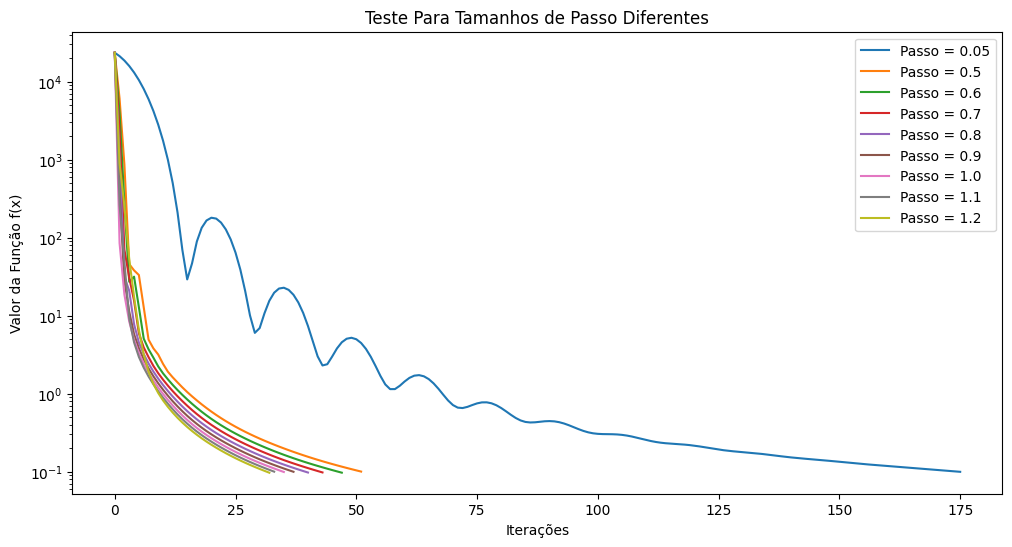
\includegraphics[width=0.8\textwidth]{tamanho_passo_semreg.png}
    \caption{Análise empírica do tamanho de passo fixo.}
    \label{fig:tamanho_passo_sreg}
\end{figure}

\begin{figure}[H]
    \centering
    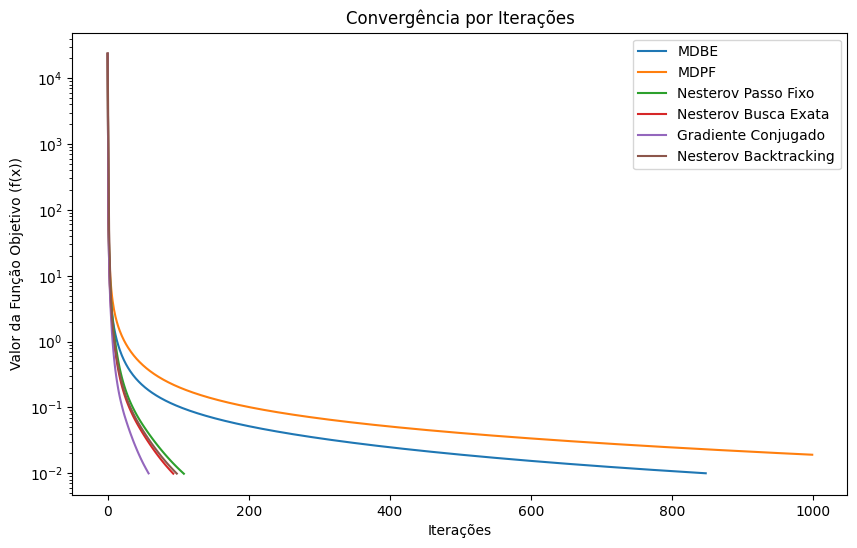
\includegraphics[width=0.8\textwidth]{conv_iter_sreg.png}
    \caption{Evolução da convergência por número de iterações.}
    \label{fig:conv_iter_sreg}
\end{figure}

\begin{figure}[H]
    \centering
    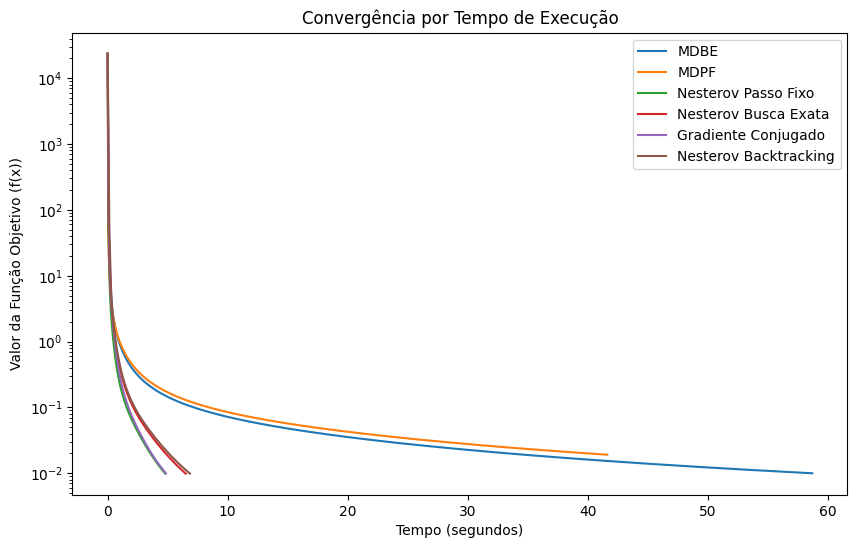
\includegraphics[width=0.8\textwidth]{conv_tempo_sreg.png}
    \caption{Evolução da convergência ao longo do tempo de execução.}
    \label{fig:conv_tempo_sreg}
\end{figure}

\begin{figure}[H]
    \centering
    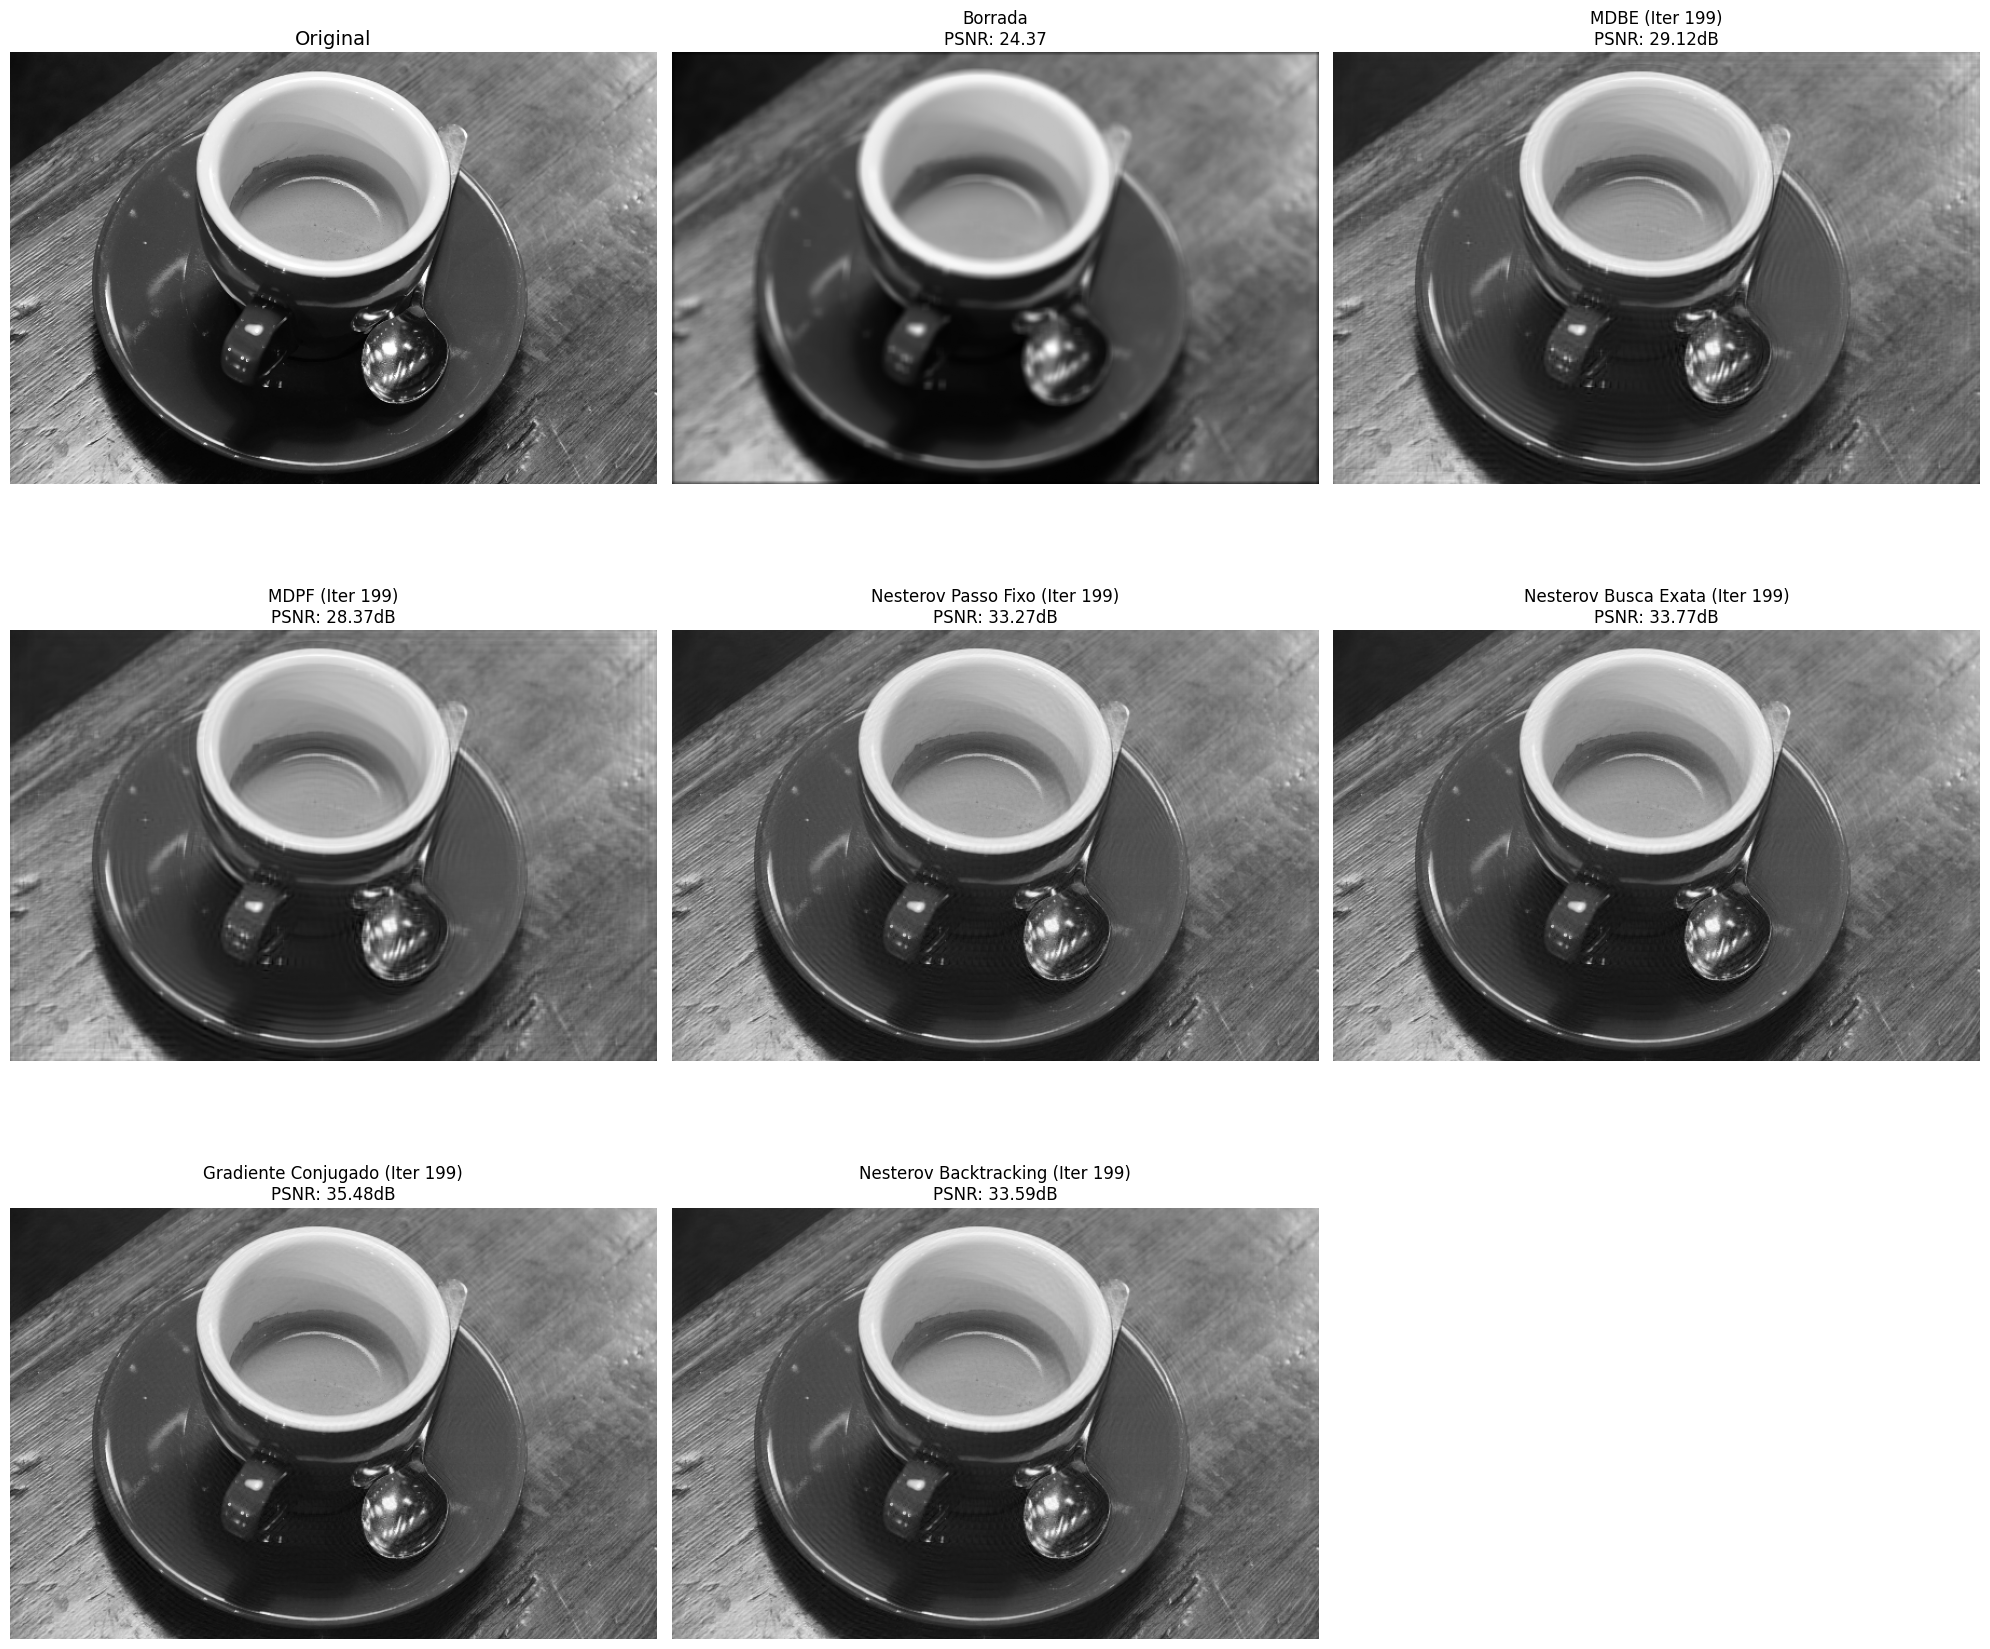
\includegraphics[width=1\textwidth]{reconstrucao_200_iter.png}
    \caption{Qualidade visual da reconstrução (200 iterações).}
    \label{fig:qual_reconst_2}  
\end{figure}

\begin{figure}[H]
    \centering
    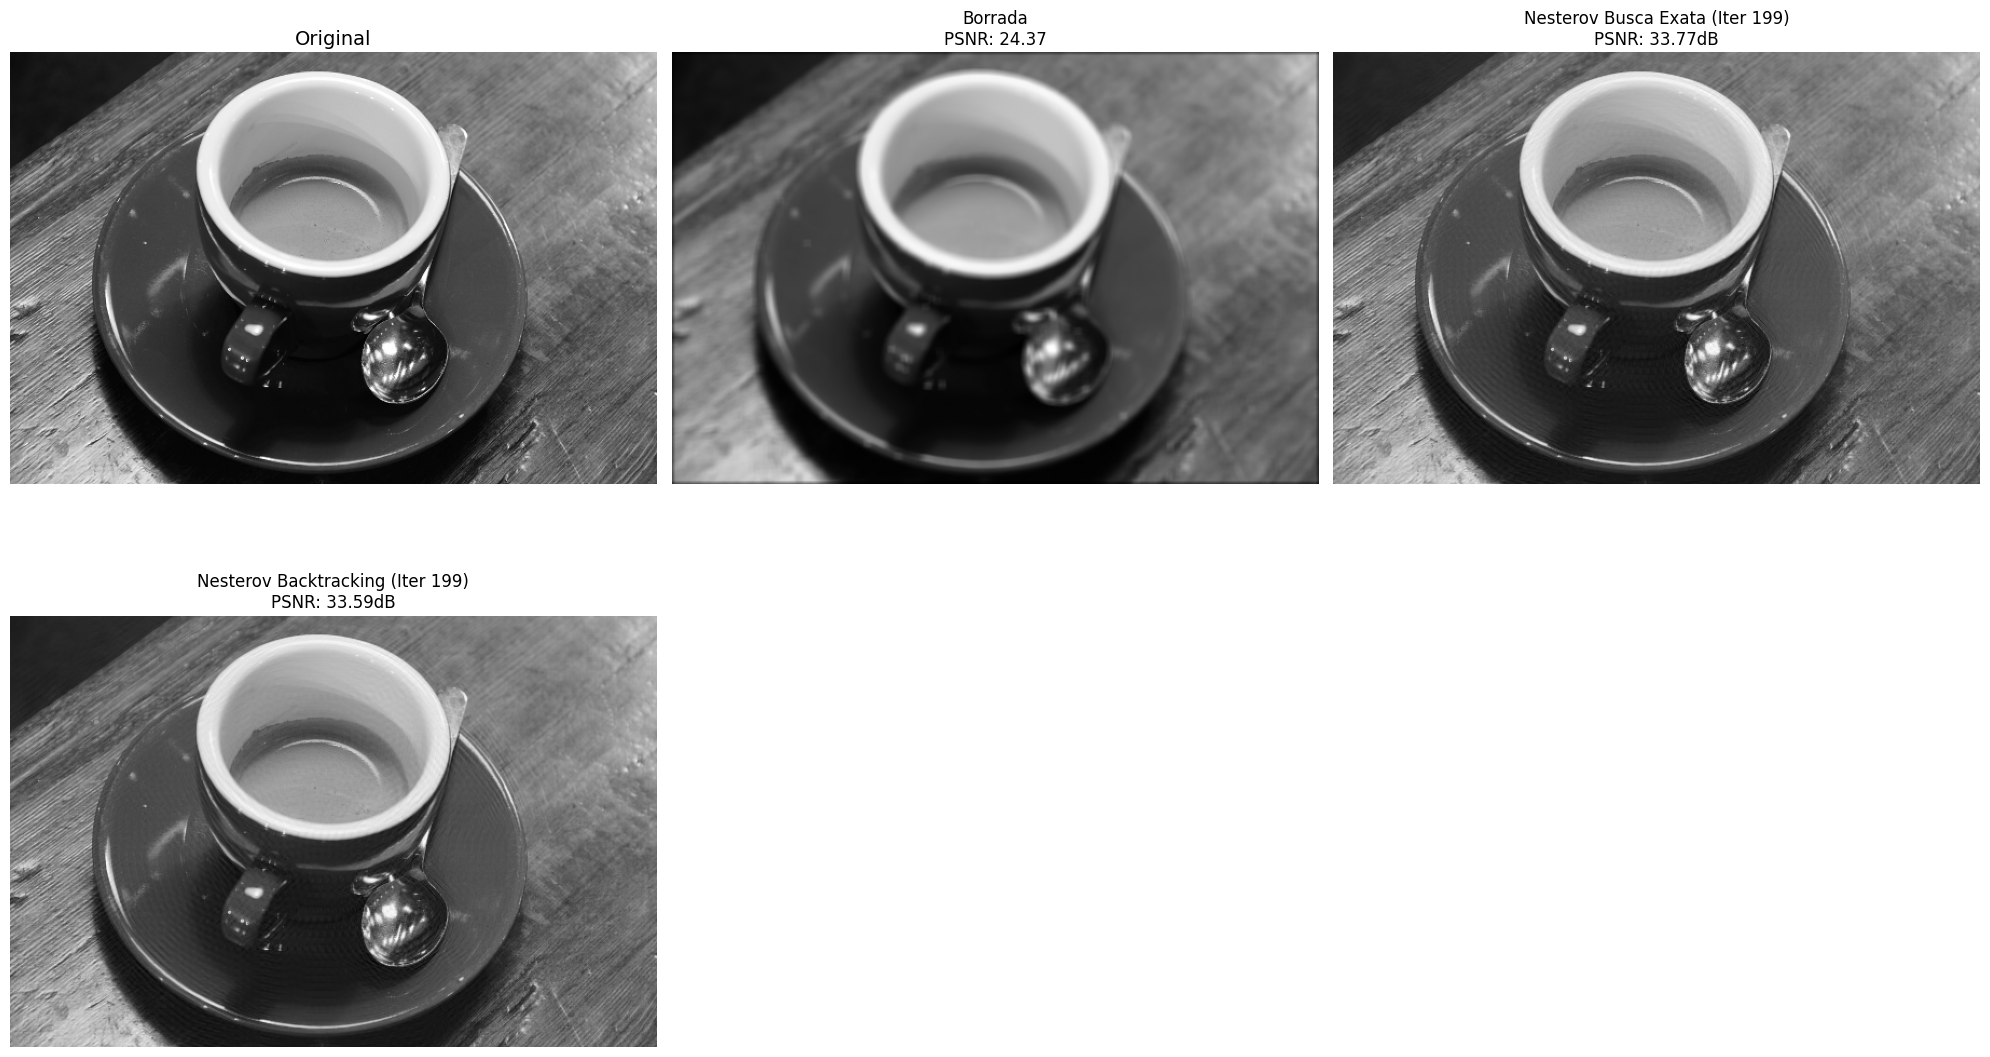
\includegraphics[width=1\textwidth]{reconstrucao_nesterov.png}
    \caption{Reconstrução sob diferentes estratégias de busca em Nesterov.}
    \label{fig:qual_reconst_nesterov}
\end{figure}

\begin{figure}[H]
    \centering
    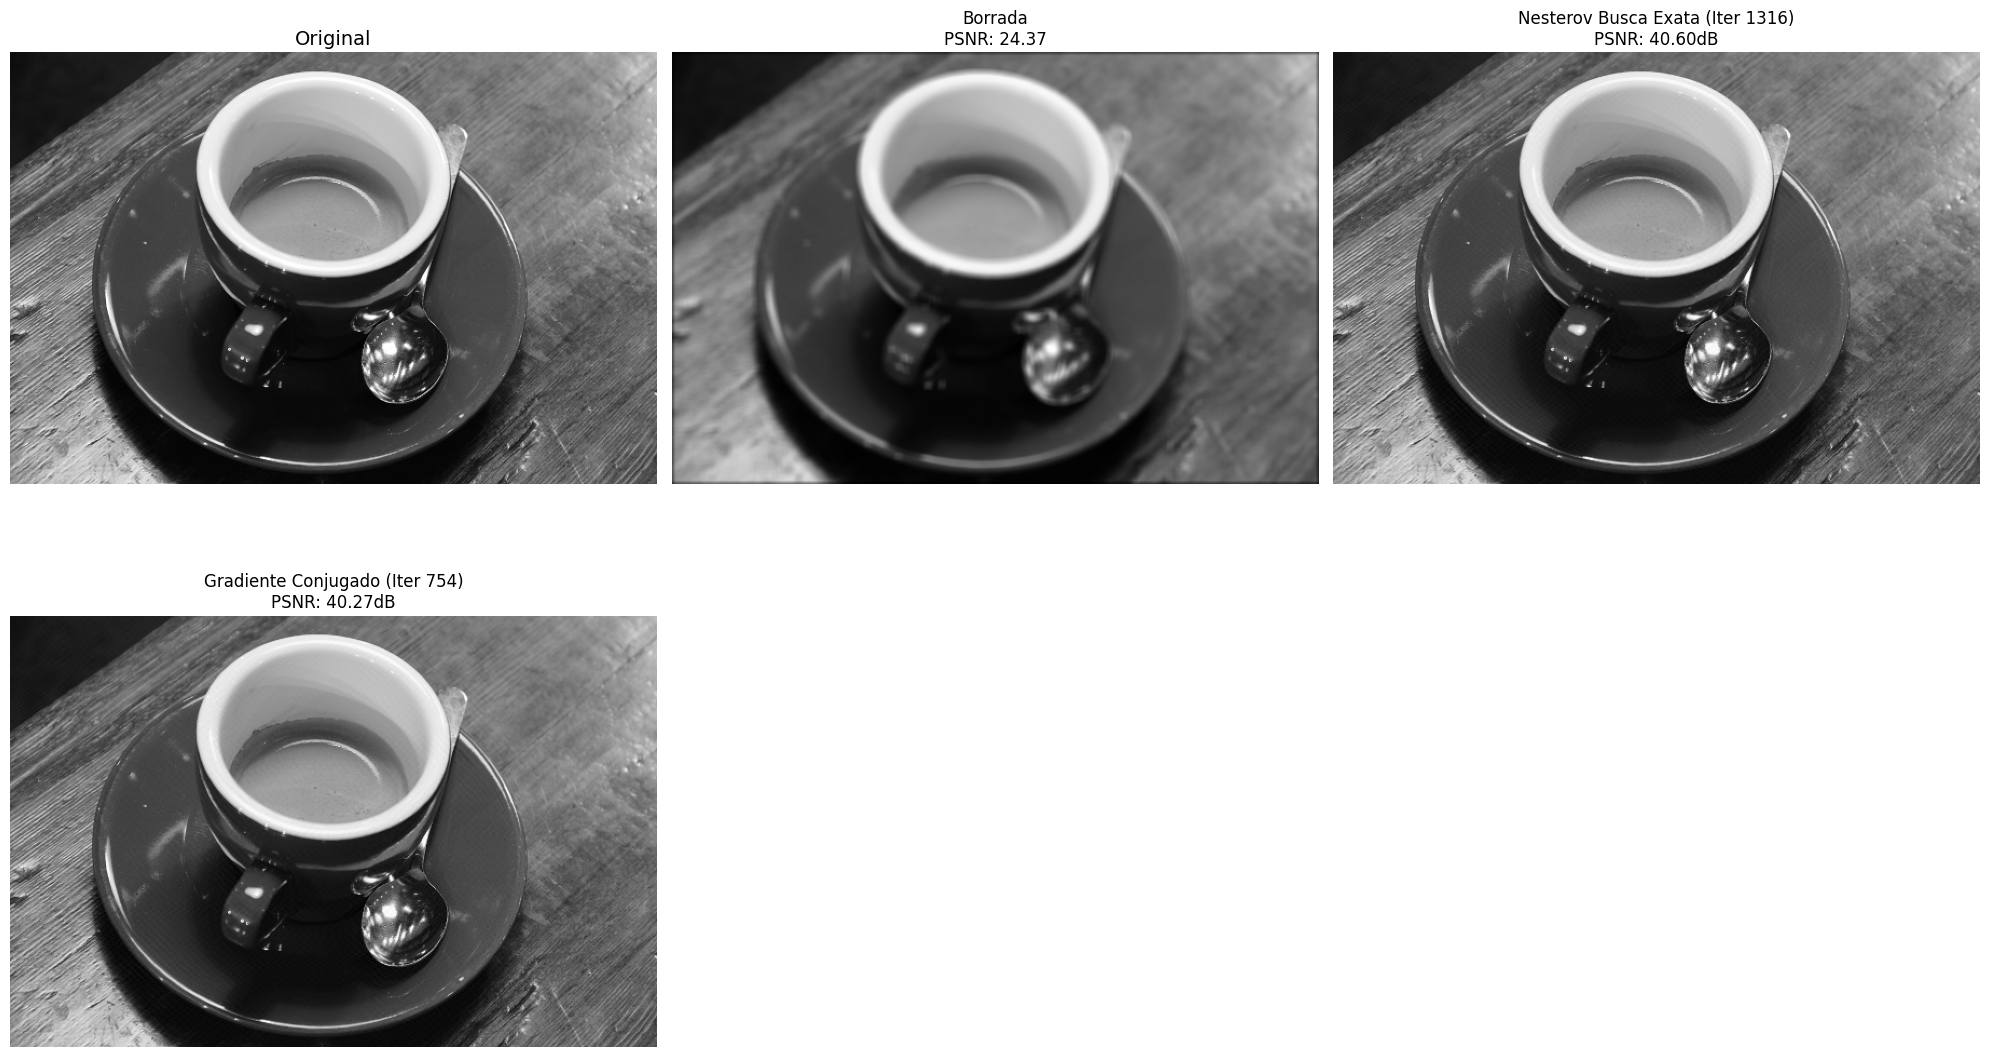
\includegraphics[width=1\textwidth]{reconstrucao_nest_gc.png}
    \caption{Reconstrução com Nesterov Busca Exata \textit{vs} Gradientes Conjugados.}
    \label{fig:reconstrucao_nest_gc}
\end{figure}

\subsection{Métodos com Regularização (\textit{Wavelets} e TV em Imagens)}


\begin{figure}[H]
    \centering
    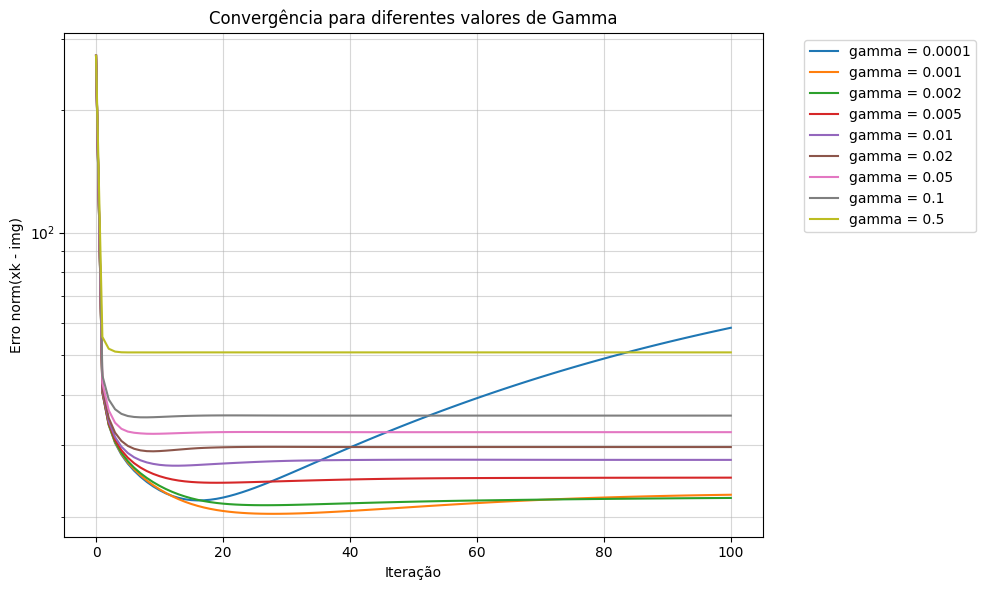
\includegraphics[width=0.8\textwidth]{grid_gamma_wav.png}
    \caption{Análise de erro (\textit{Grid-Search}) para determinação do parâmetro ótimo $\gamma=0.001$ (\textit{Wavelets}).}
    \label{fig:grid_wav.png}
\end{figure}


\begin{figure}[H]
    \centering
    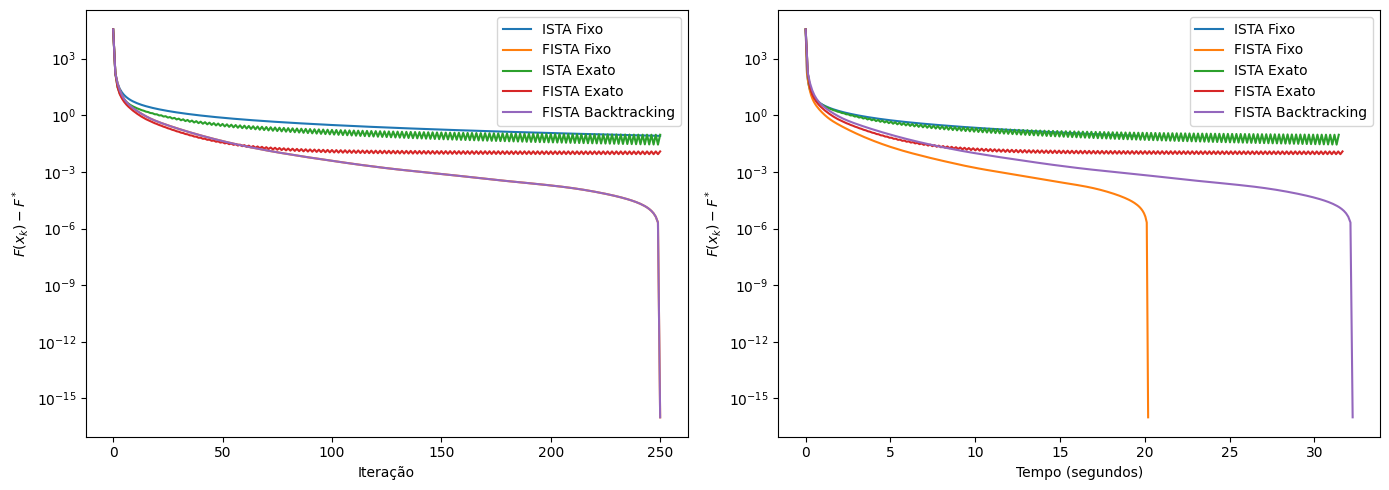
\includegraphics[width=1\textwidth]{f_fstar1.png}
    \caption{Convergência de $F(x_k) - F(x^*)$ ao longo do tempo (\textit{Wavelets}).}
    \label{fig:f_fstar1}
\end{figure}

\begin{figure}[H]
    \centering
    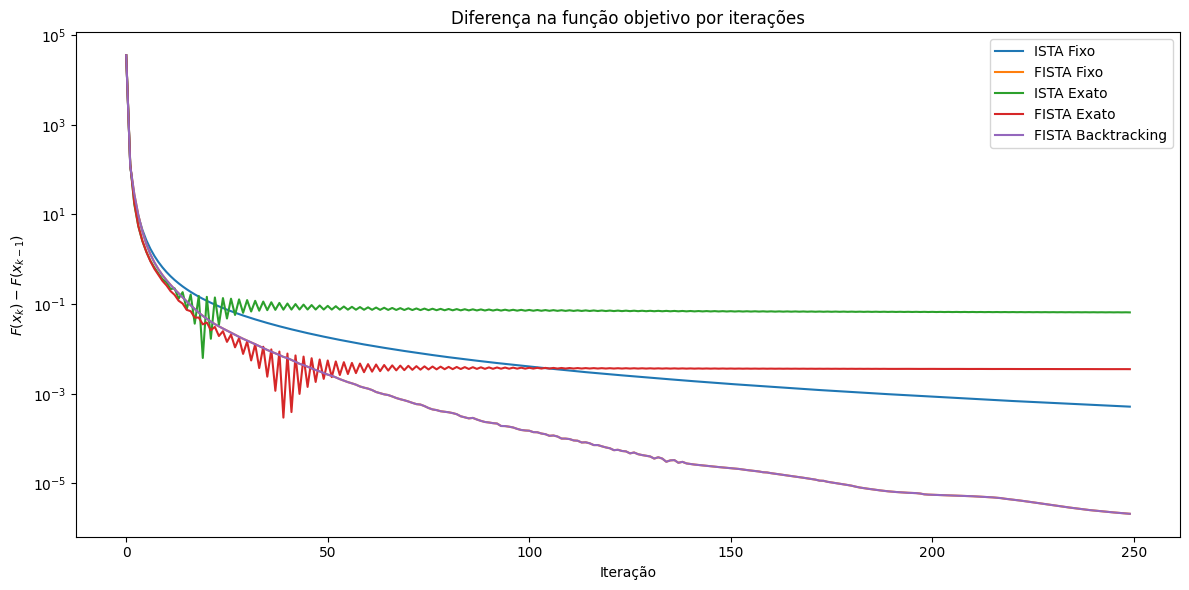
\includegraphics[width=1\textwidth]{fk1_fk.png}
    \caption{Variação dos iterados $F(x_k) - F(x_{k-1})$ (\textit{Wavelets}).}
    \label{fig:fk1_fk}
\end{figure}

\begin{figure}[H]
    \centering
    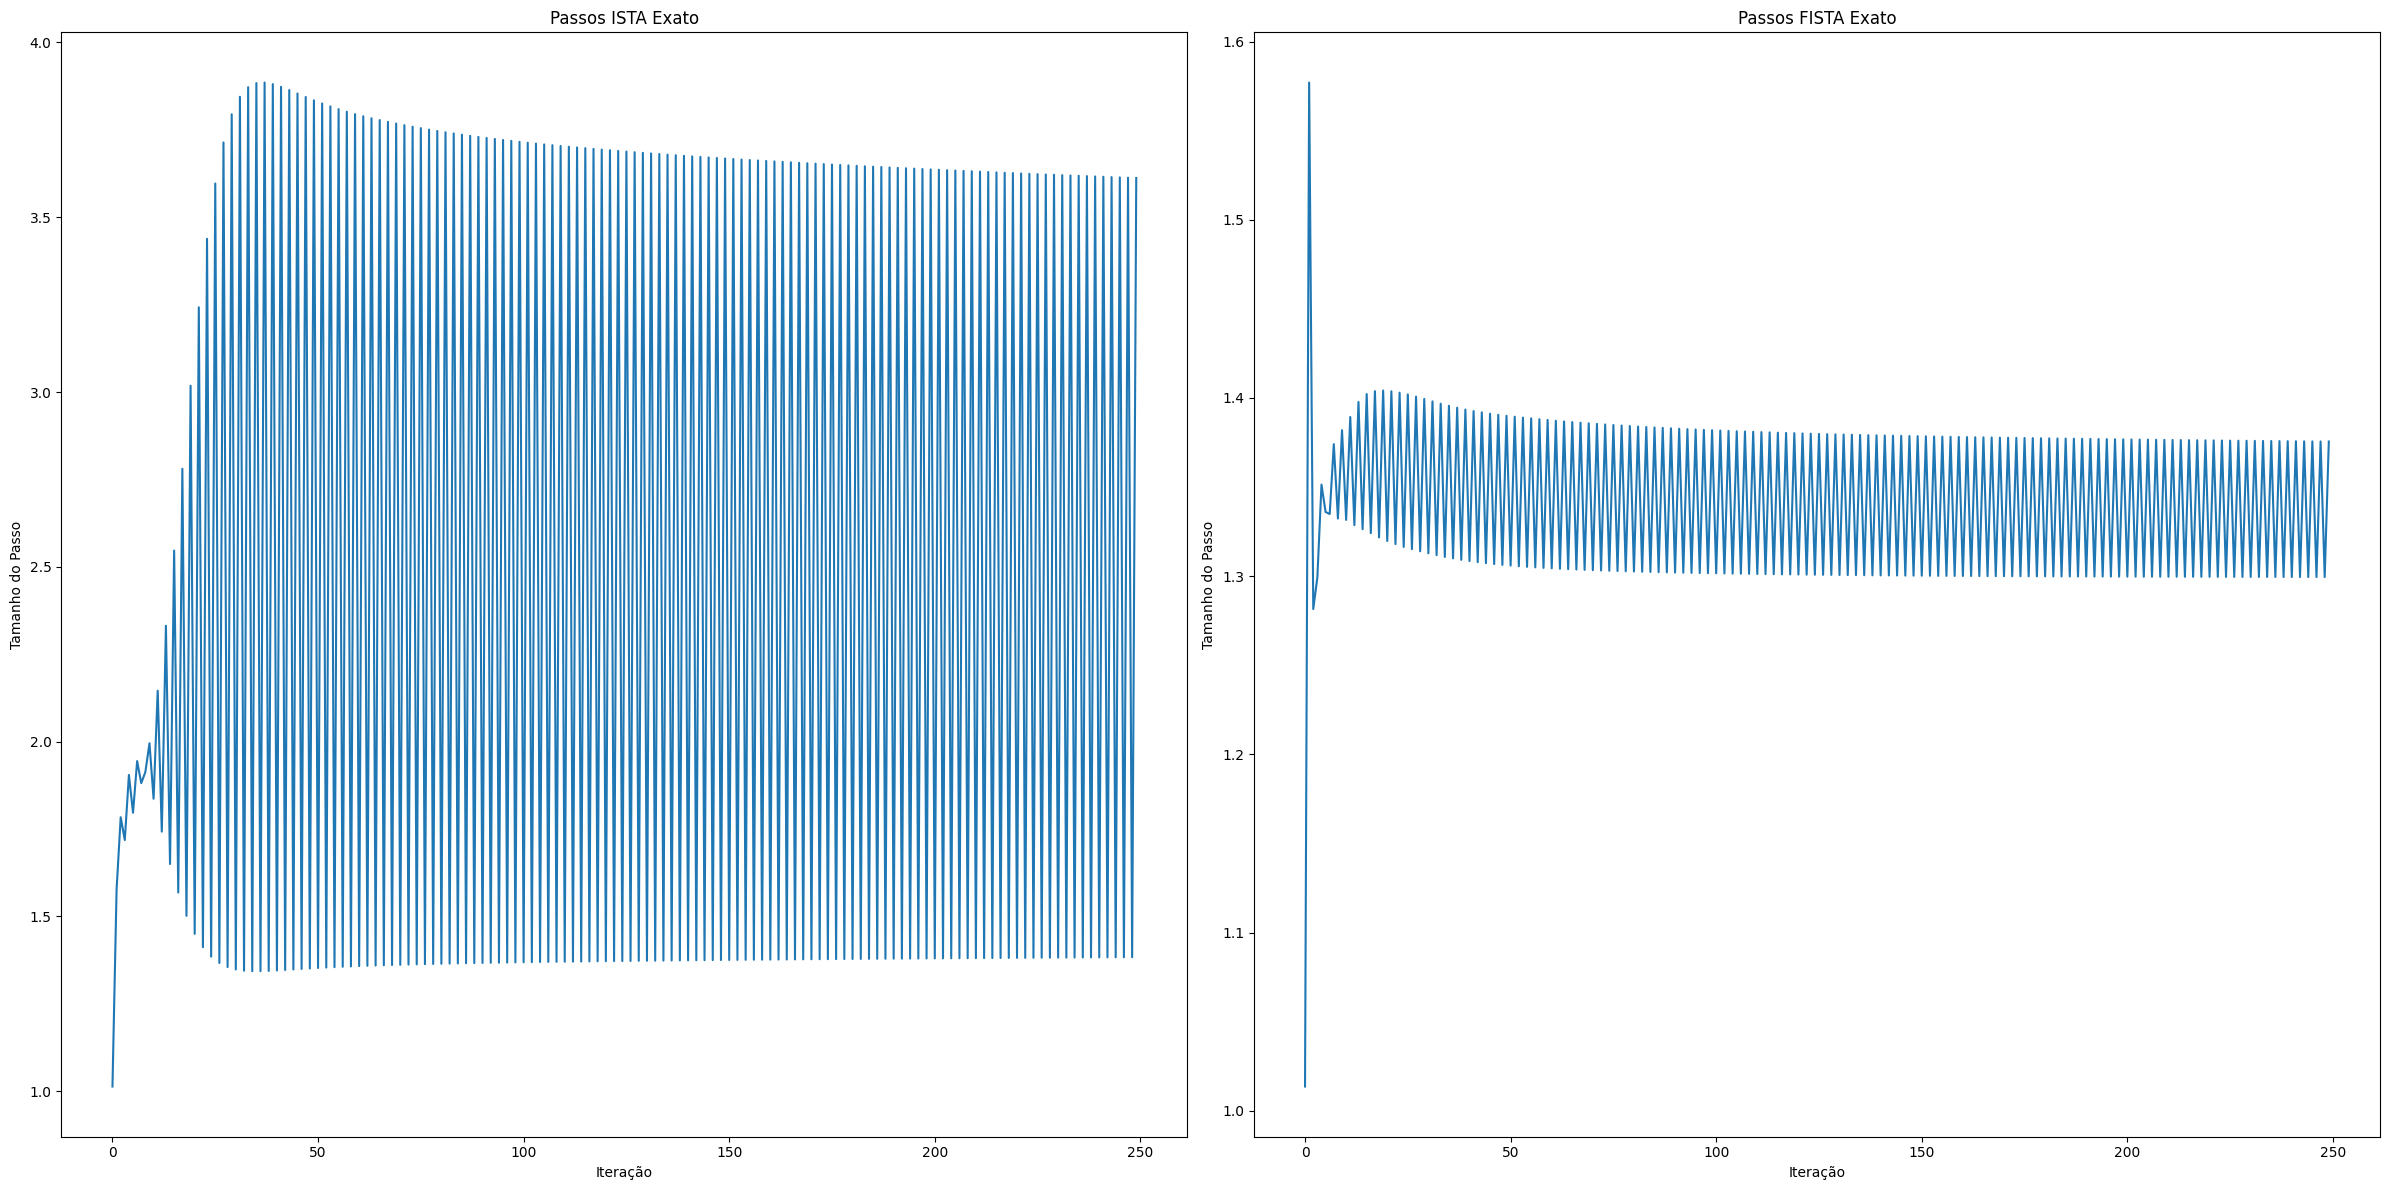
\includegraphics[width=0.8\textwidth]{tamanho_passo_creg.png}
    \caption{Tamanho de passo em modelos com $\gamma = 0.001$ (\textit{Wavelets}).} 
    \label{fig:tamanho_passo_creg}
\end{figure}

\begin{figure}[H]
    \centering
    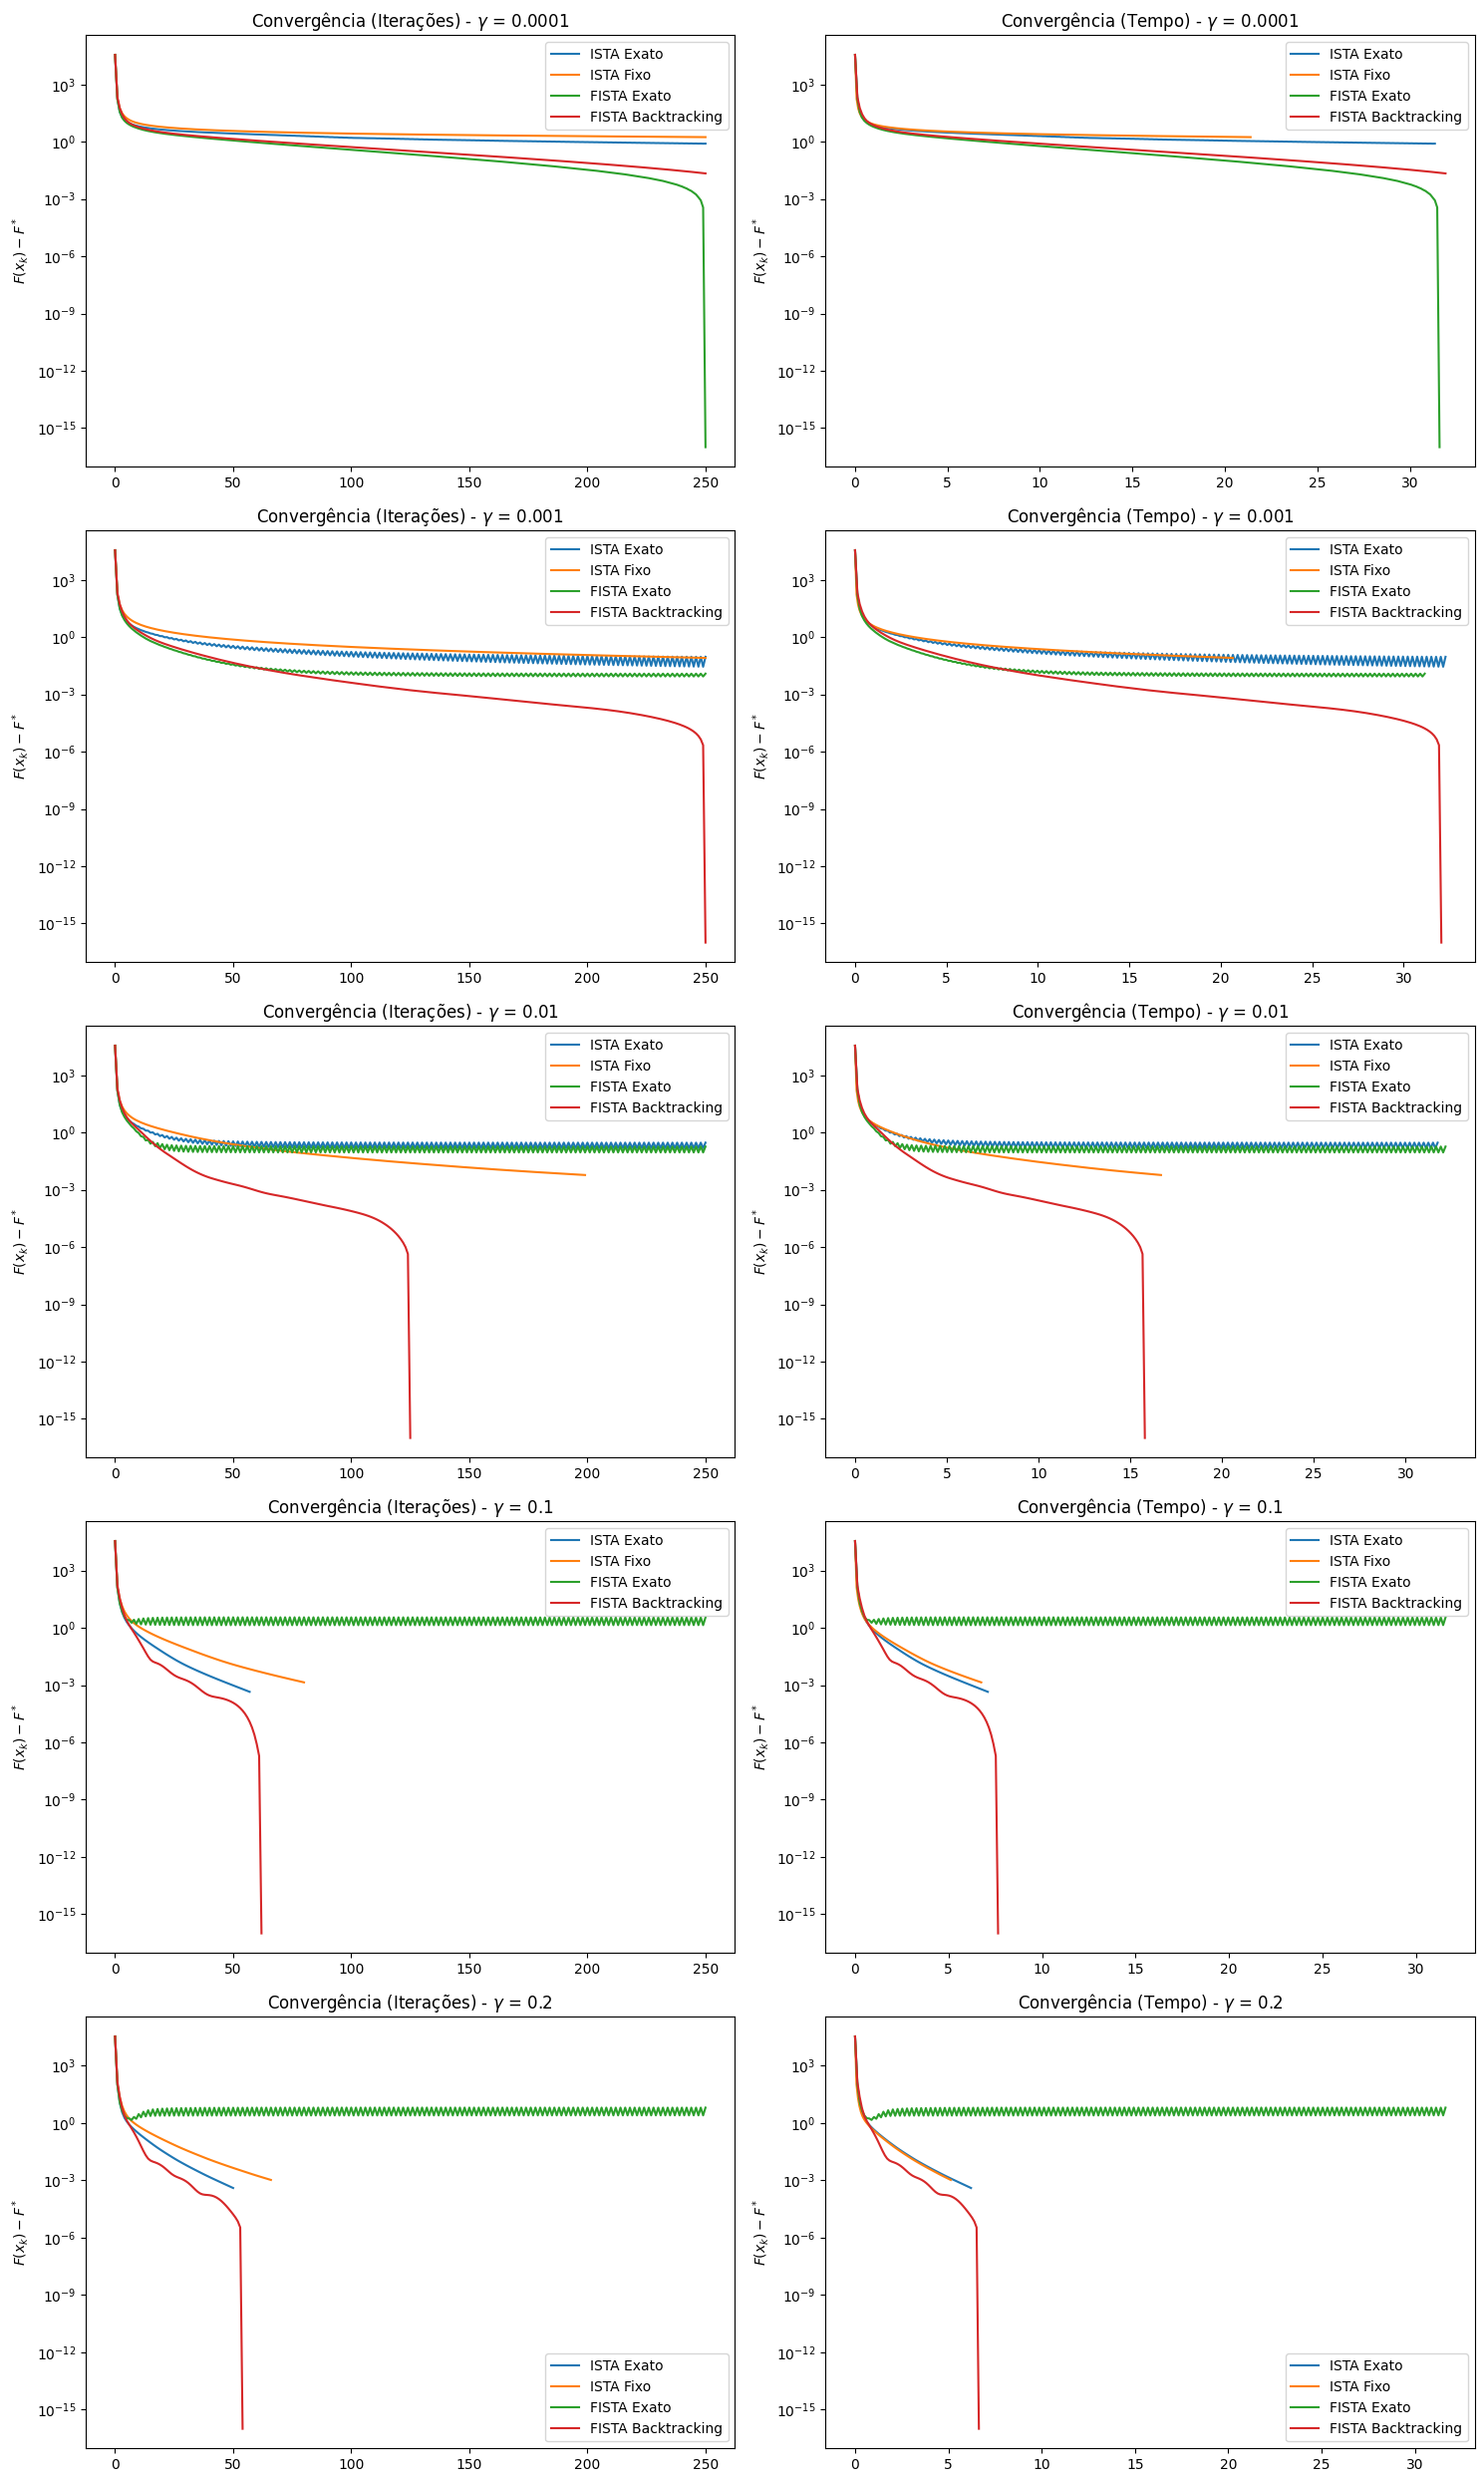
\includegraphics[width=0.8\textwidth]{testes1_creg.png}
    \caption{Impacto de diferentes valores de $\gamma$ na distância ao ótimo $F(x^*)$ (\textit{Wavelets}).}
    \label{fig:testes1}
\end{figure}

\begin{figure}[H]
    \centering
    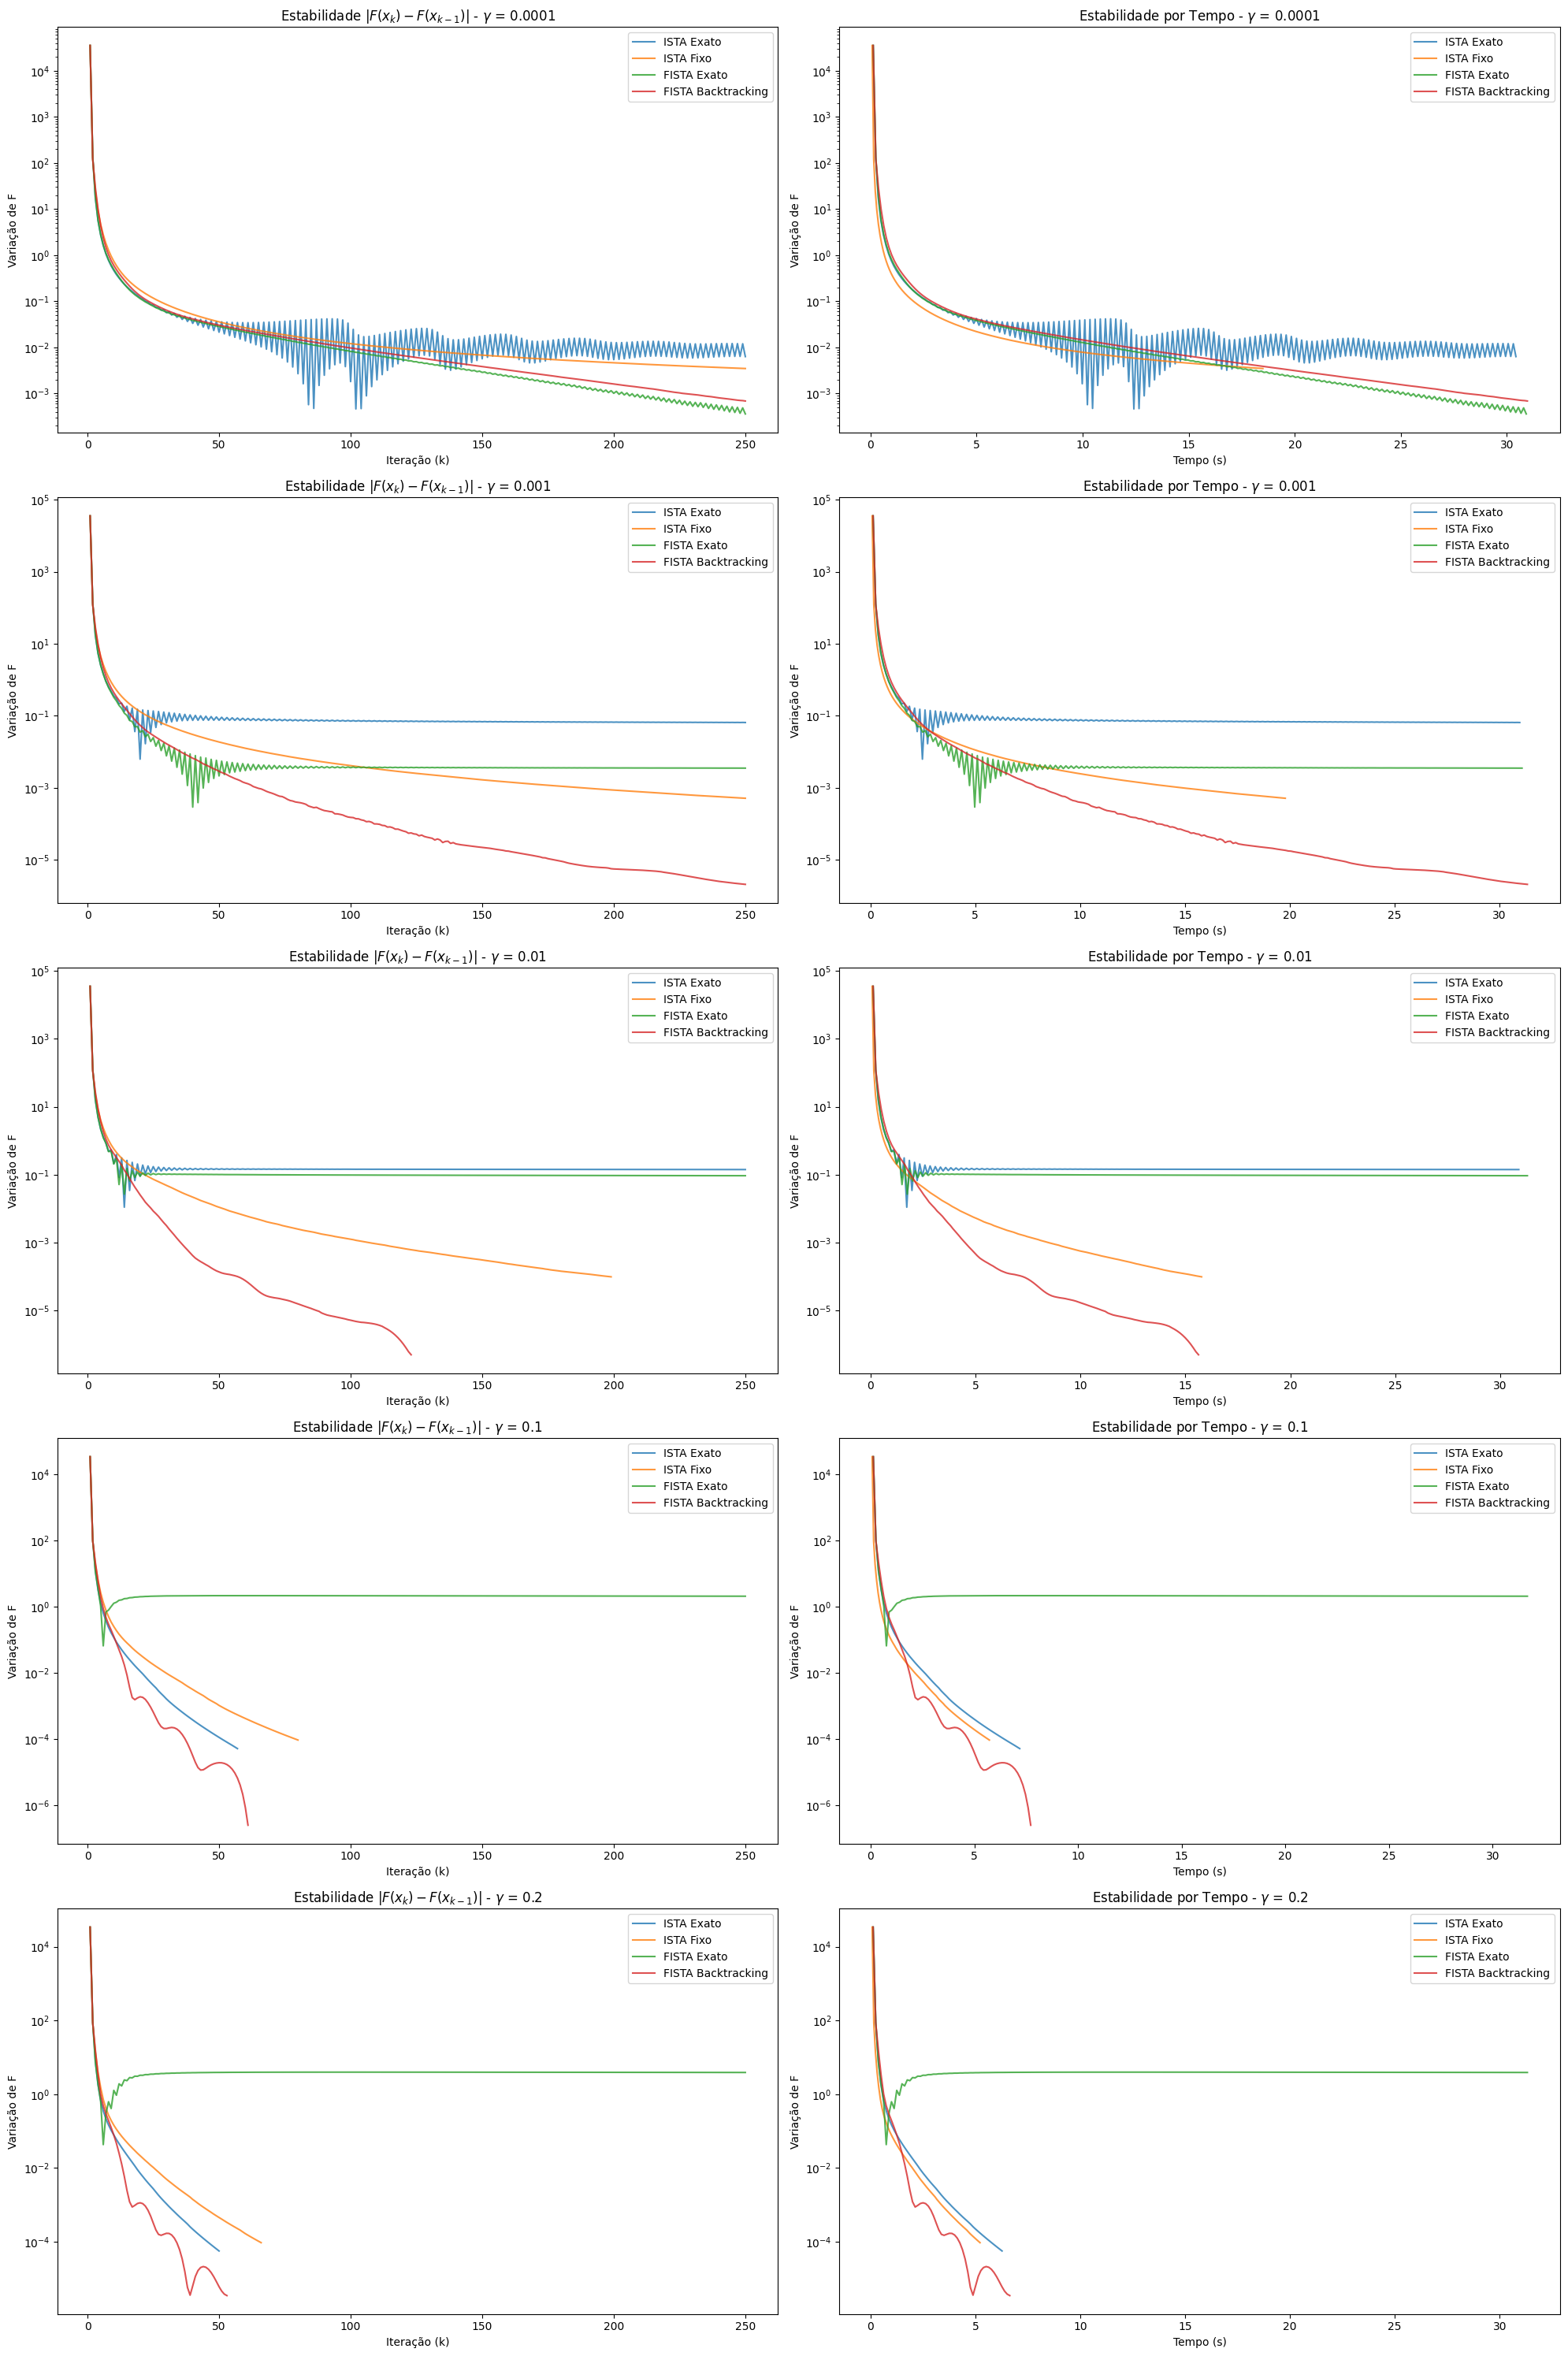
\includegraphics[width=0.8\textwidth]{testes2_creg.png}
    \caption{Estabilidade iterativa para diferentes valores de $\gamma$ (\textit{Wavelets}).}
    \label{fig:testes2}
\end{figure}

% \begin{figure}[H]
%     \centering
%     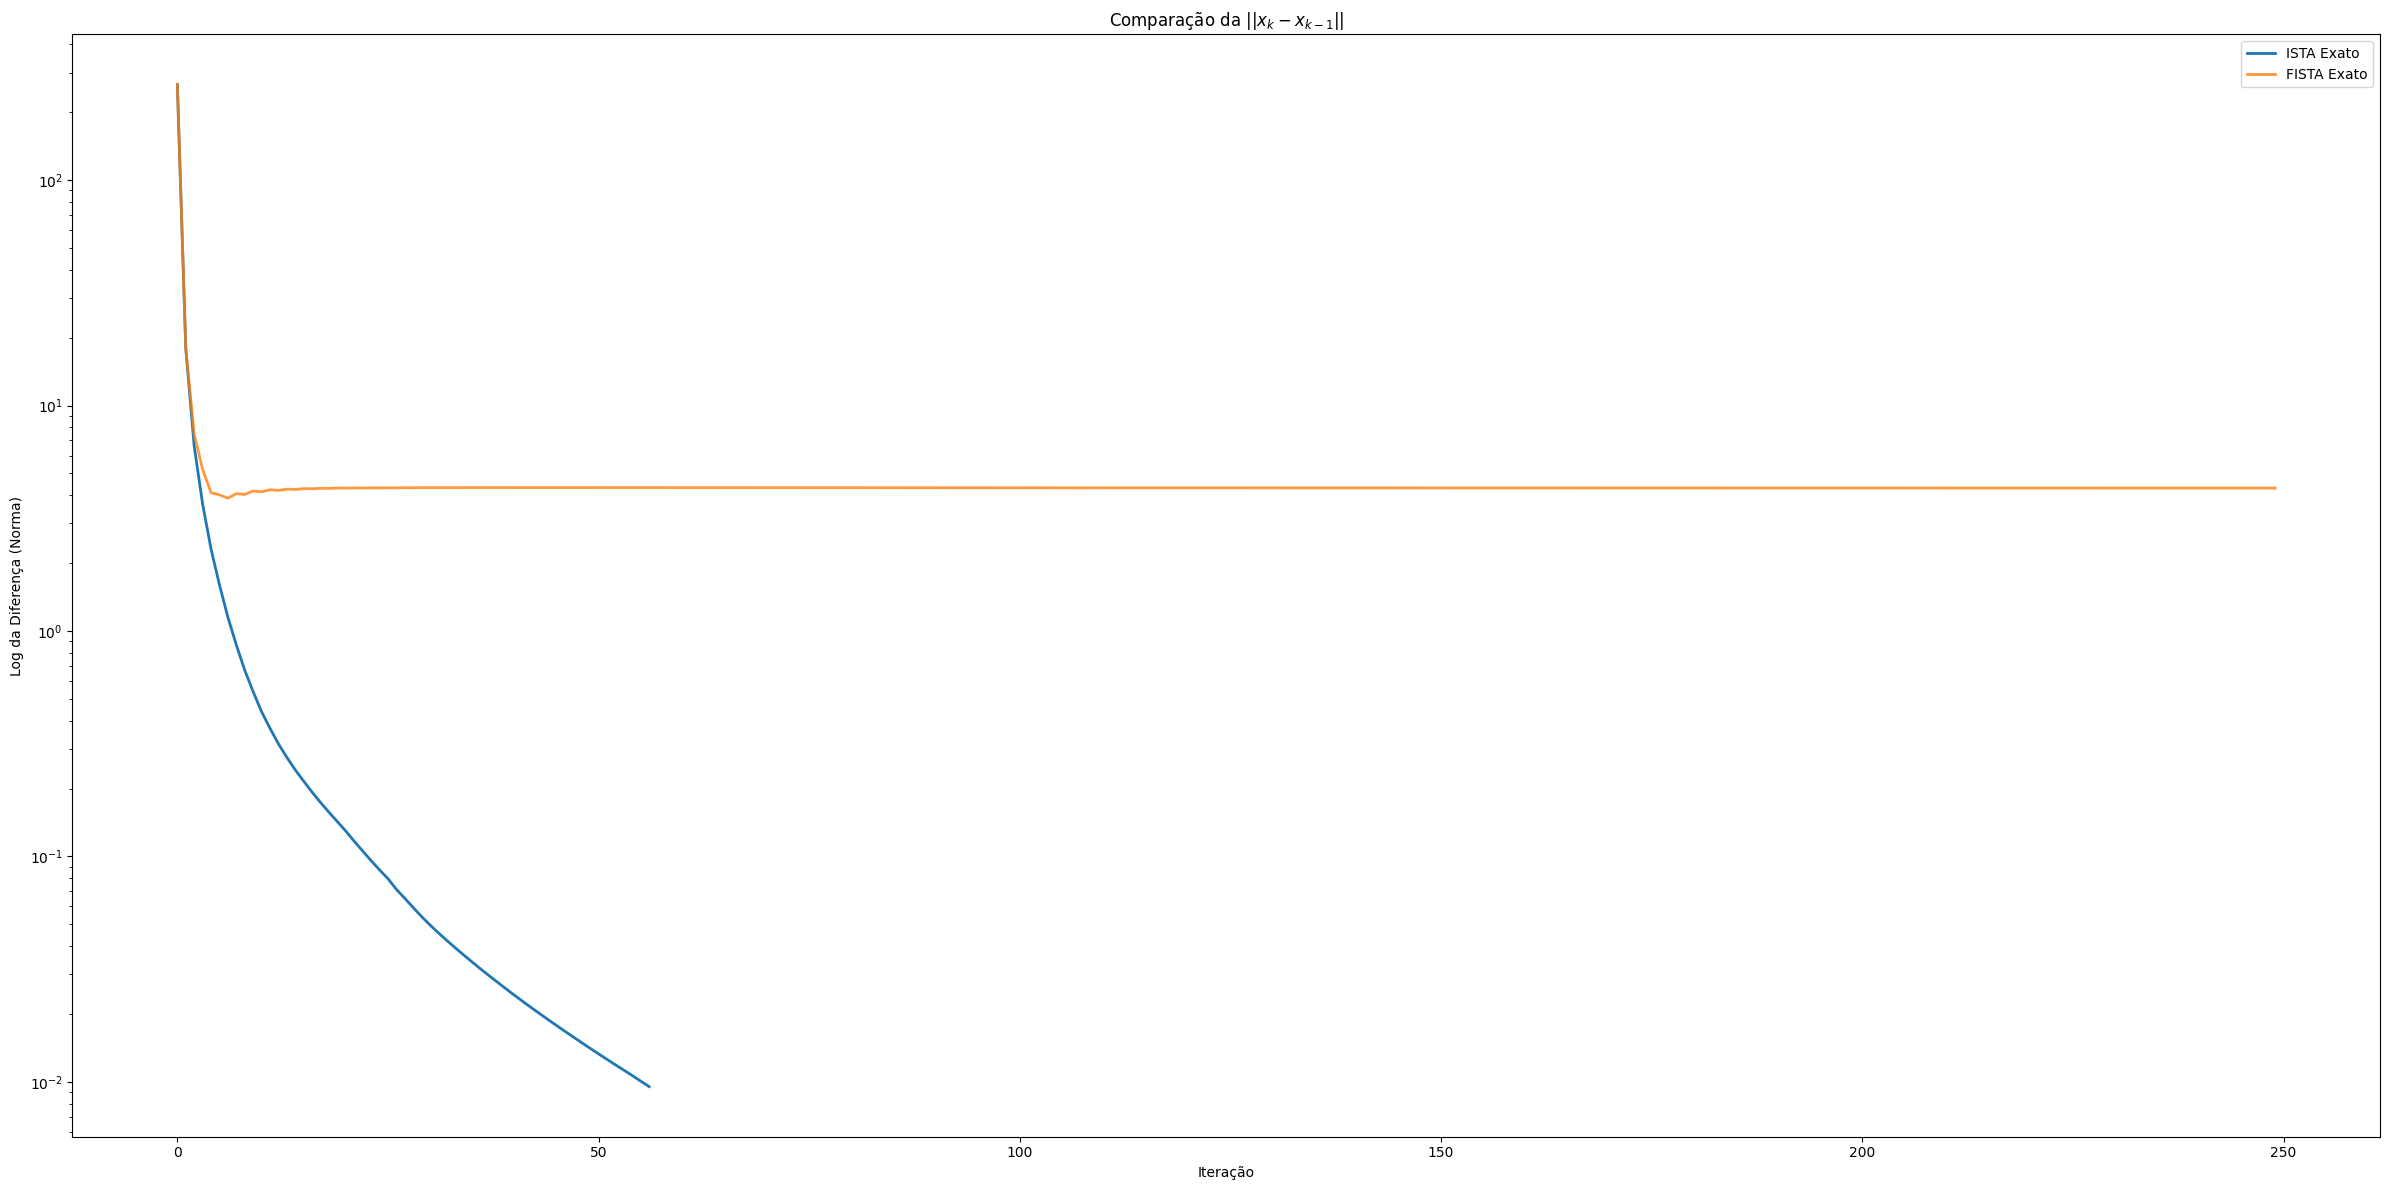
\includegraphics[width=0.9\textwidth]{norm_xk1_xk.png}
%     \caption{Estabilidade de ISTA e FISTA em alto grau regularizador ($\gamma=0.1$).}
%     \label{fig:norm_diff}
% \end{figure}

% \begin{figure}[H]
%     \centering
%     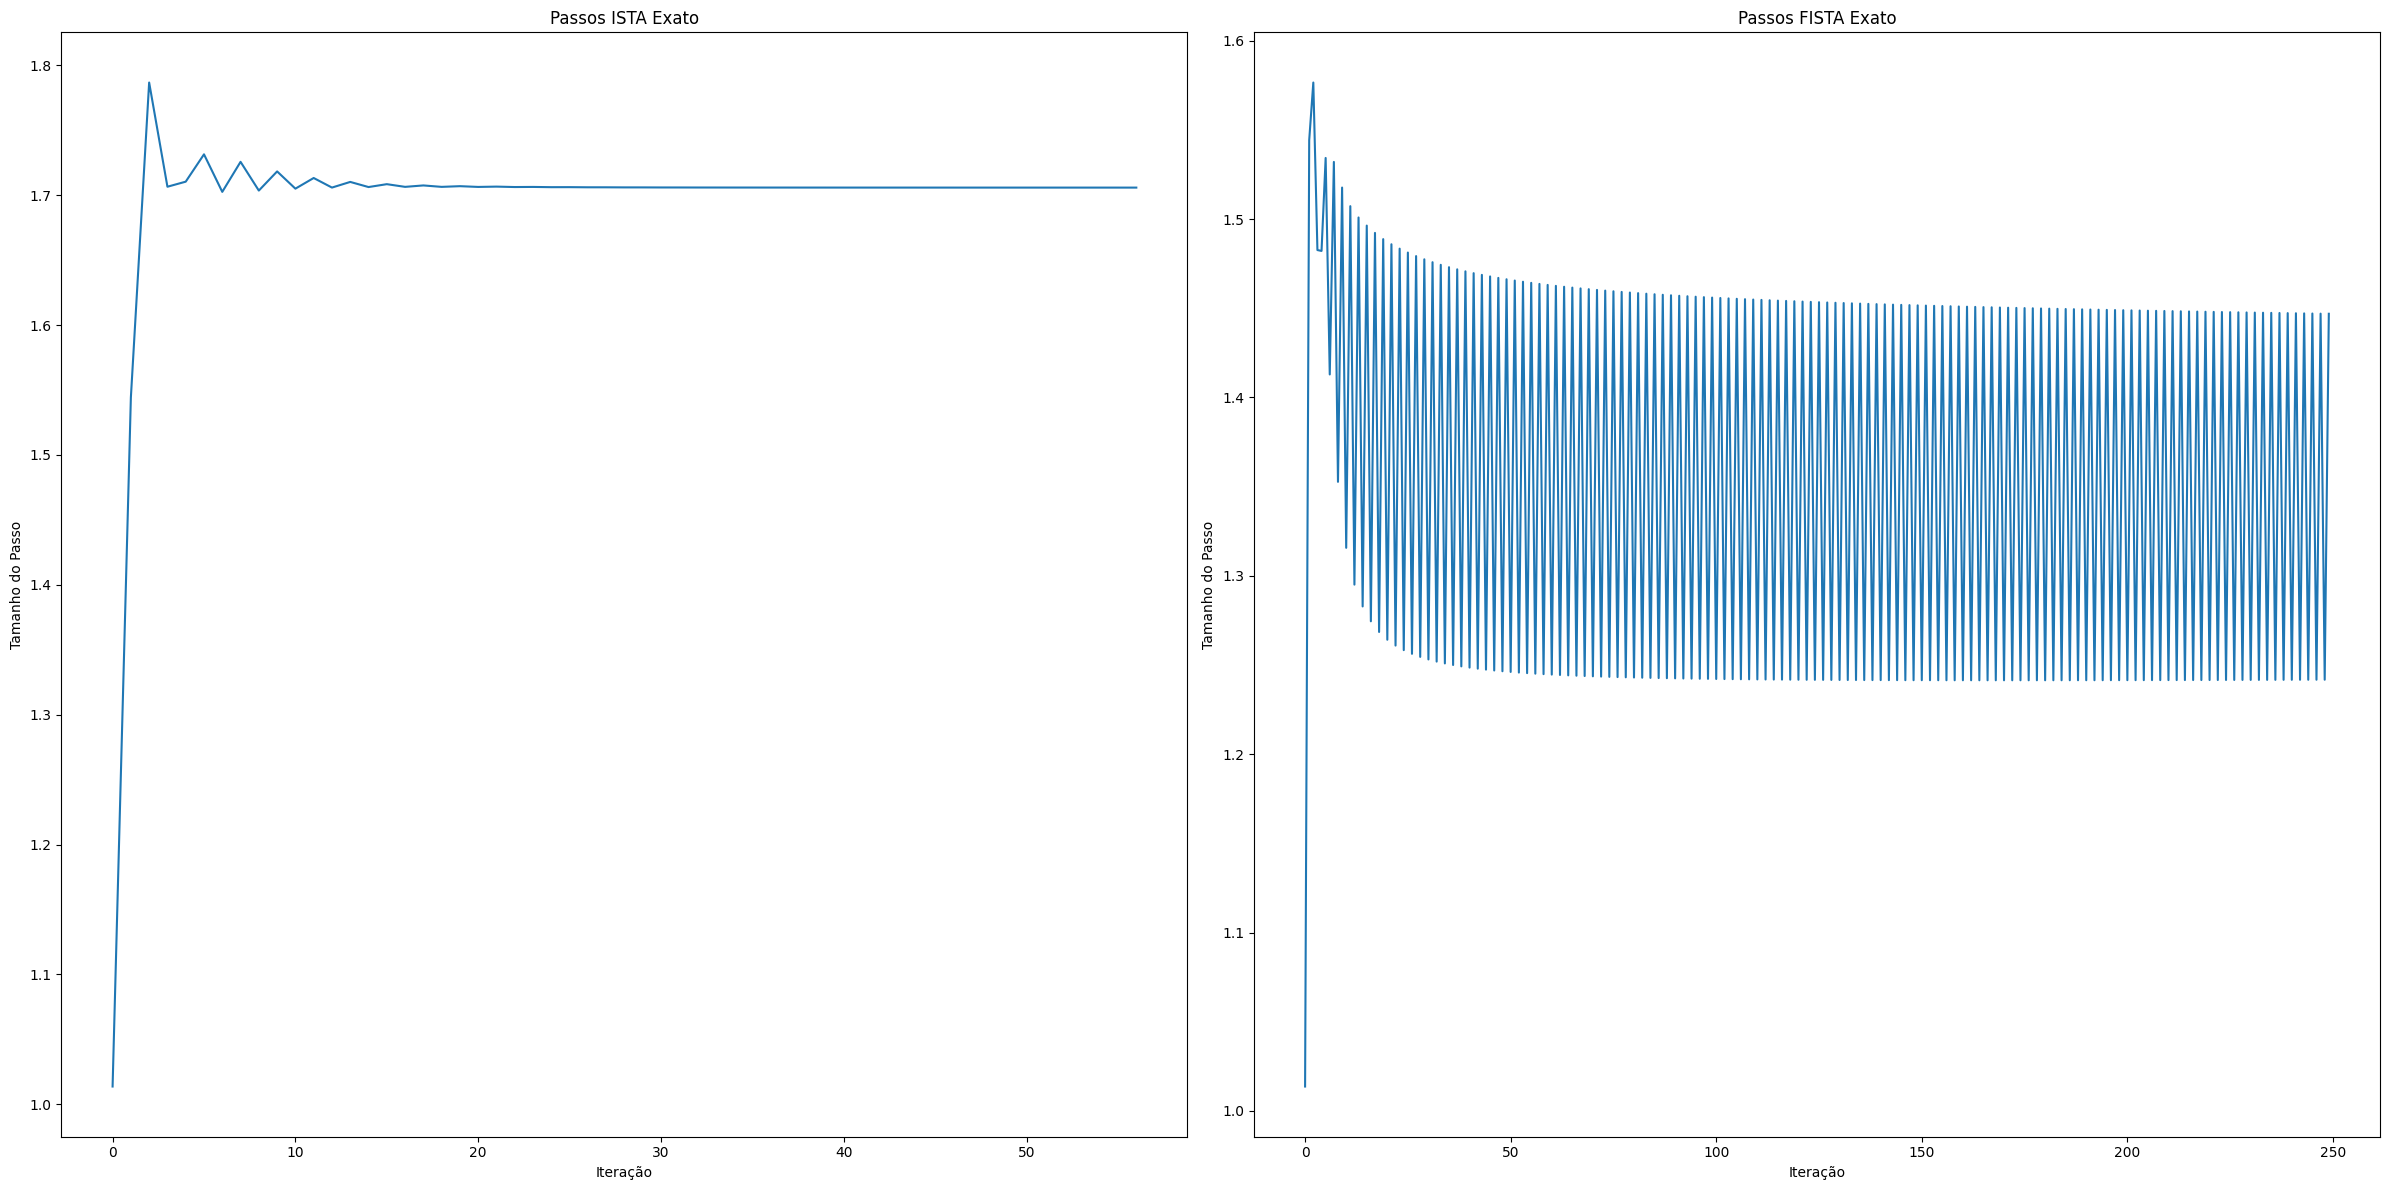
\includegraphics[width=0.9\textwidth]{passos_gamma_grande.png}
%     \caption{Tamanho de passo em ISTA/FISTA para $\gamma=0.1$.}
%     \label{fig:passos_gamma_grande}
% \end{figure}

\begin{figure}[H]
    \centering
    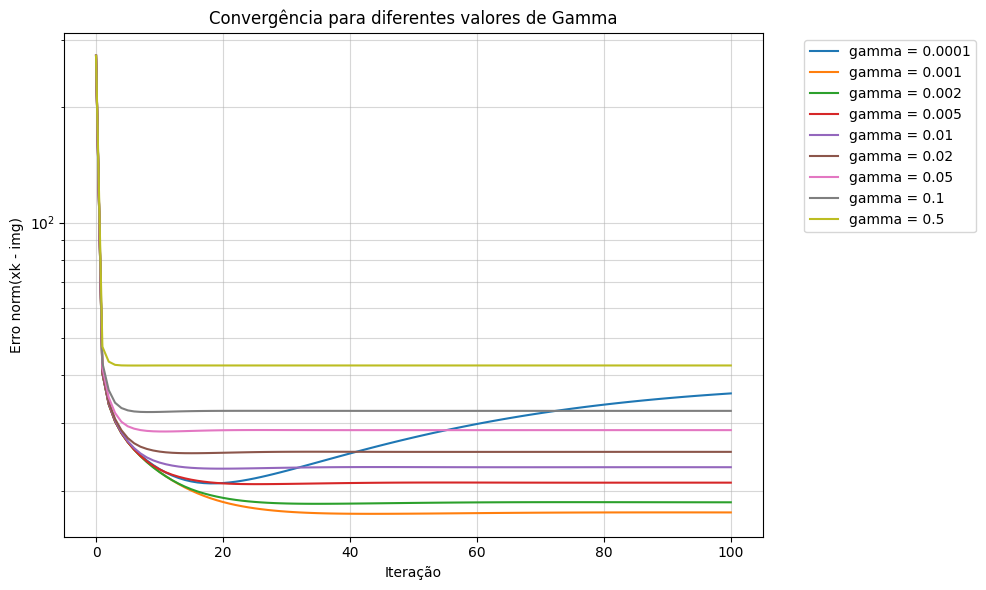
\includegraphics[width=0.8\textwidth]{grid_tv.png}
    \caption{\textit{Grid-Search} para determinação do parâmetro ótimo $\gamma=0.001$ (Variação Total).}
    \label{fig:grid_tv.png}
\end{figure}

\begin{figure}[H]
    \centering
    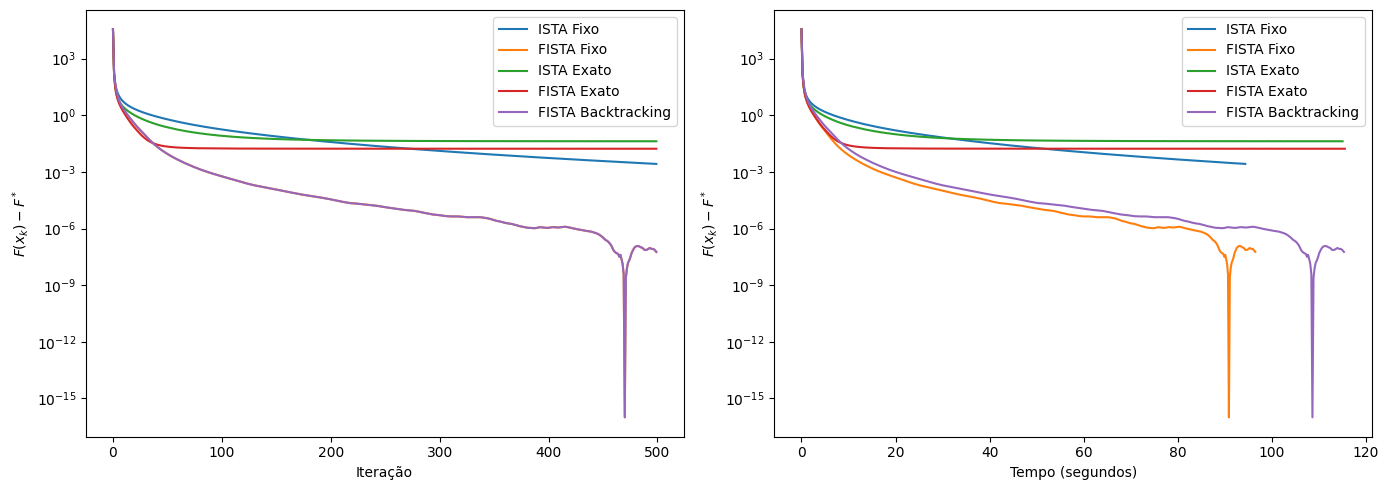
\includegraphics[width=1\textwidth]{decaimento_iter_otimo_tv.png}
    \caption{Convergência de $F(x_k) - F(x^*)$ ao longo do tempo para $\gamma=0.001$ (Variação Total).}
    \label{fig:decaimento_iter_otimo_tv.png}
\end{figure}

\begin{figure}[H]
    \centering
    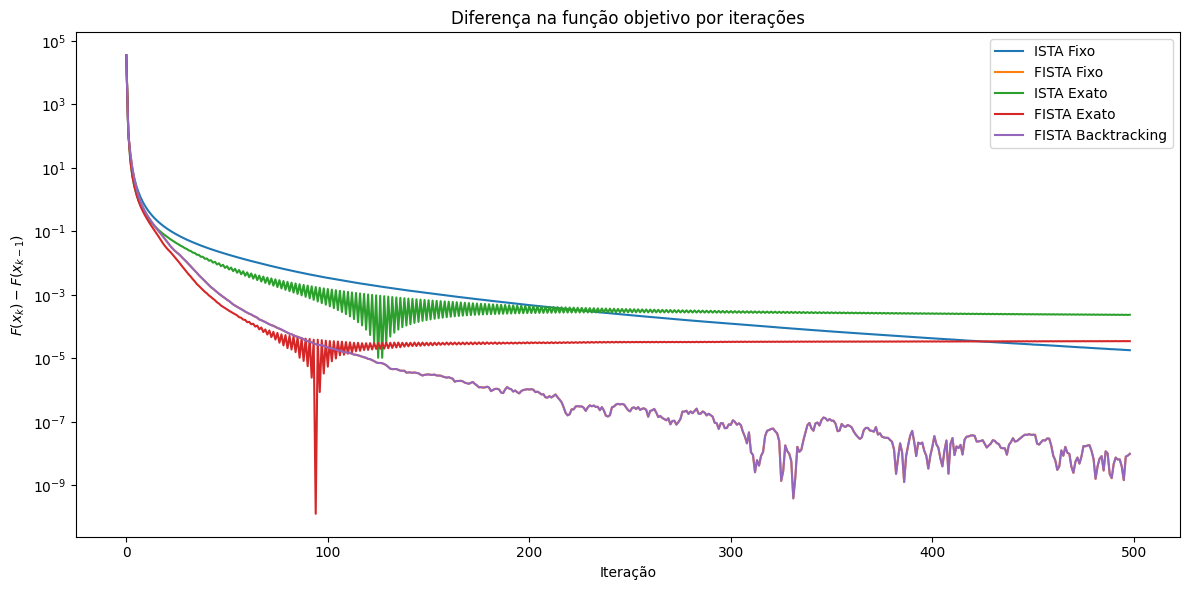
\includegraphics[width=1\textwidth]{decaimento_iters_tv.png}
    \caption{Variação dos iterados $F(x_k) - F(x_{k-1})$ para $\gamma=0.001$ (Variação Total).}
    \label{fig:decaimento_iters_tv.png}
\end{figure}

\begin{figure}[H]
    \centering
    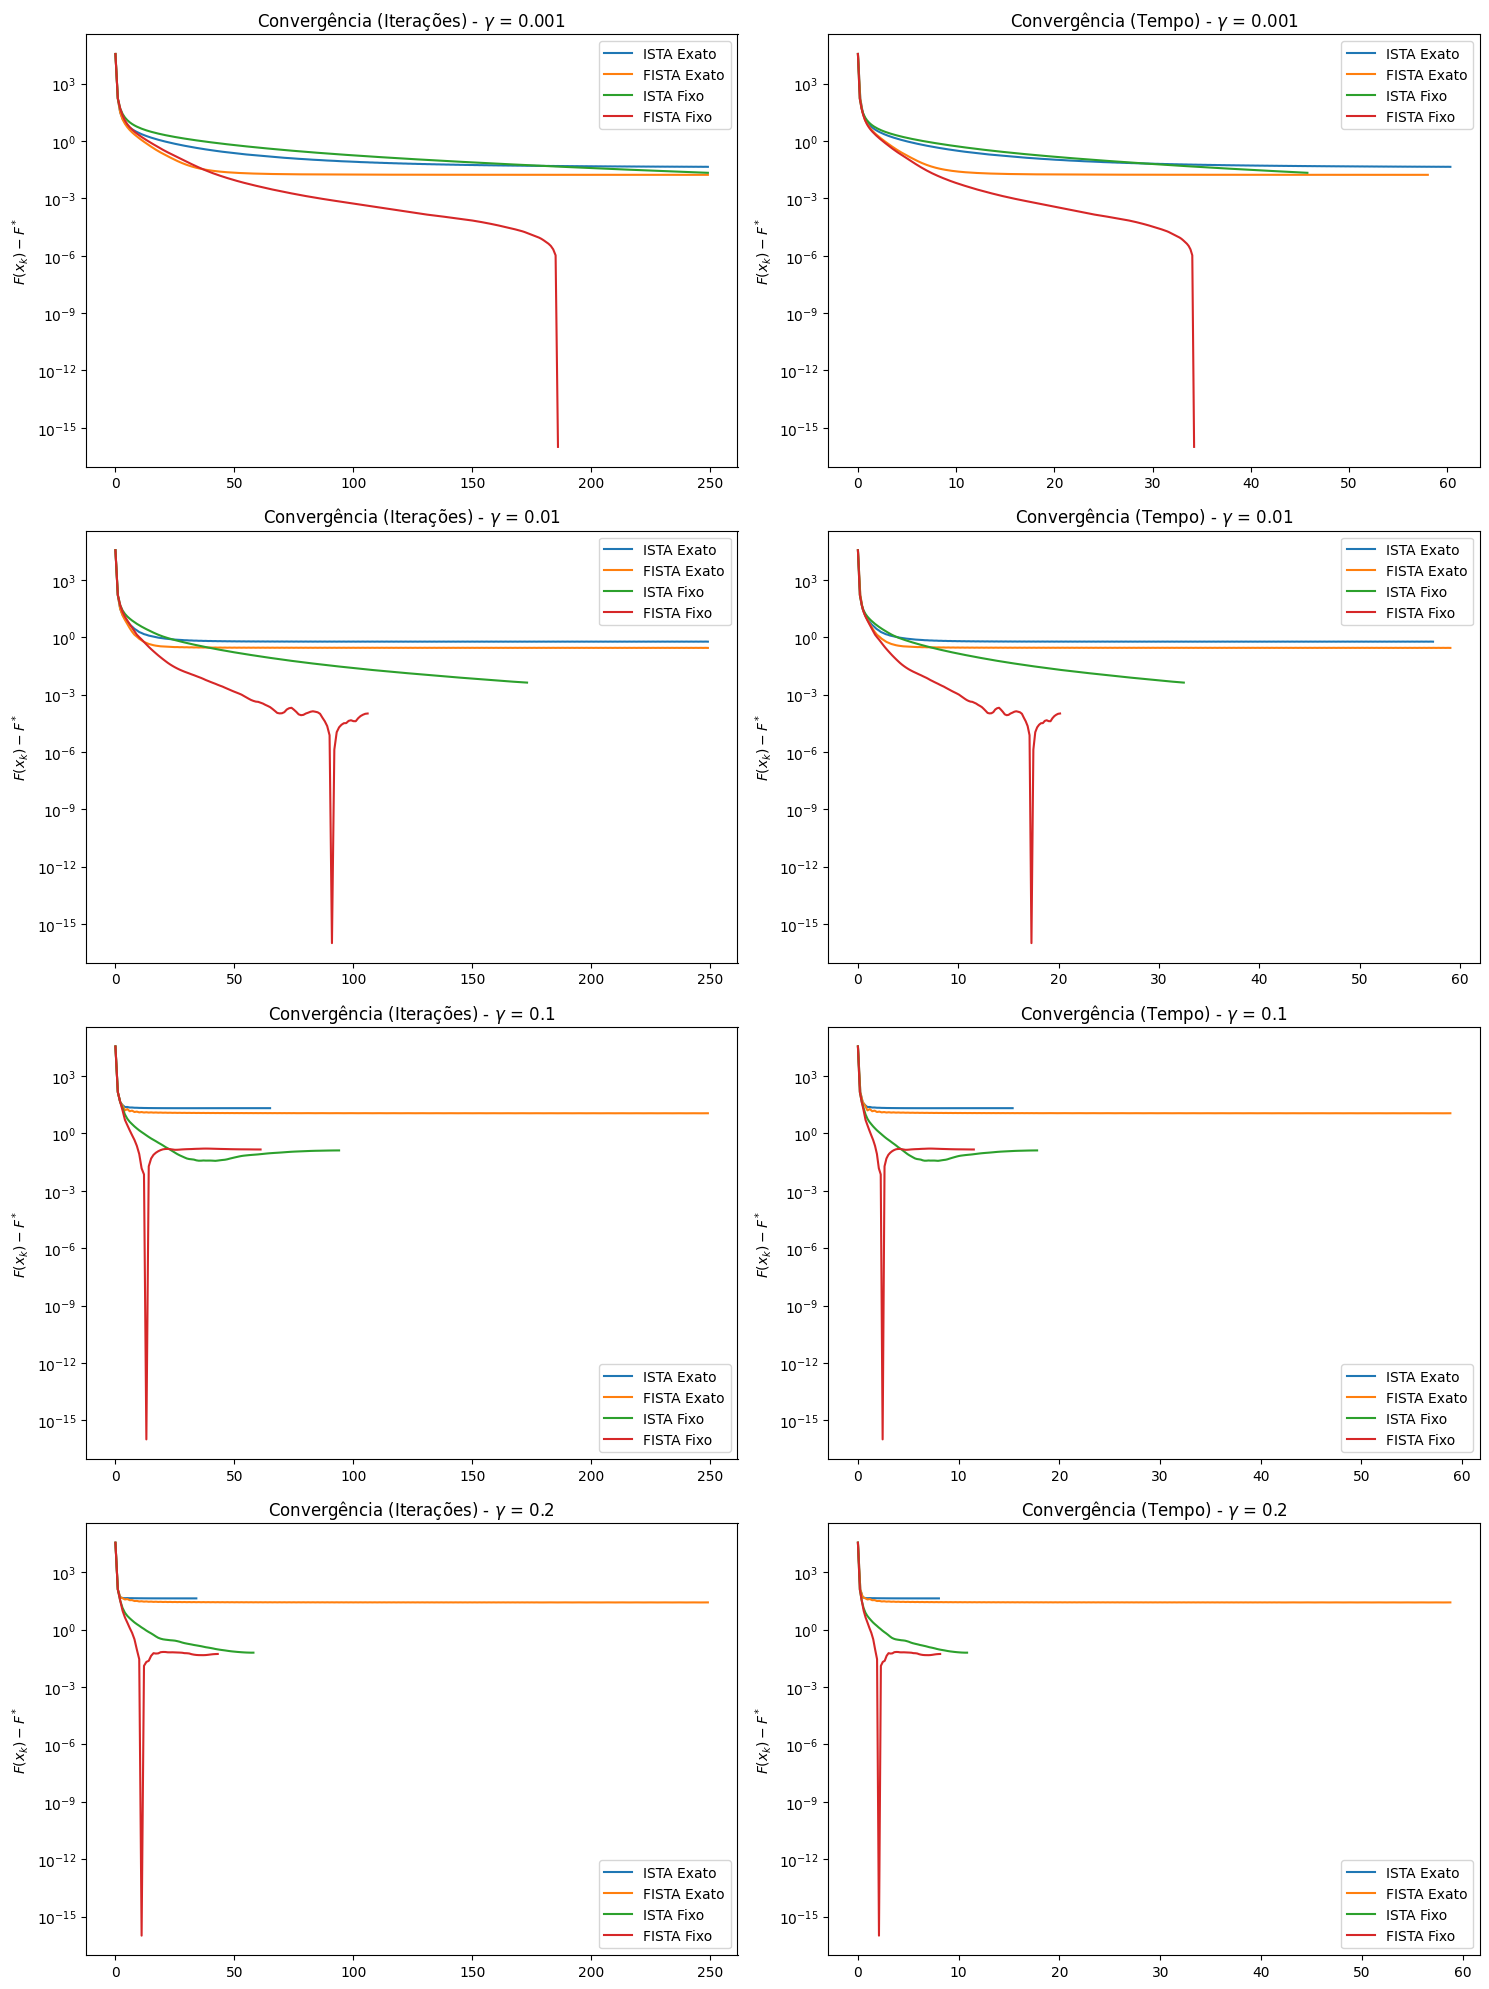
\includegraphics[width=0.8\textwidth]{comp_gammas_tv.png}
    \caption{Impacto de diferentes valores de $\gamma$ na distância ao ótimo $F(x^*)$ (Variação Total).}
    \label{fig:comp_gamma_tv}
\end{figure}

\begin{figure}[H]
    \centering
    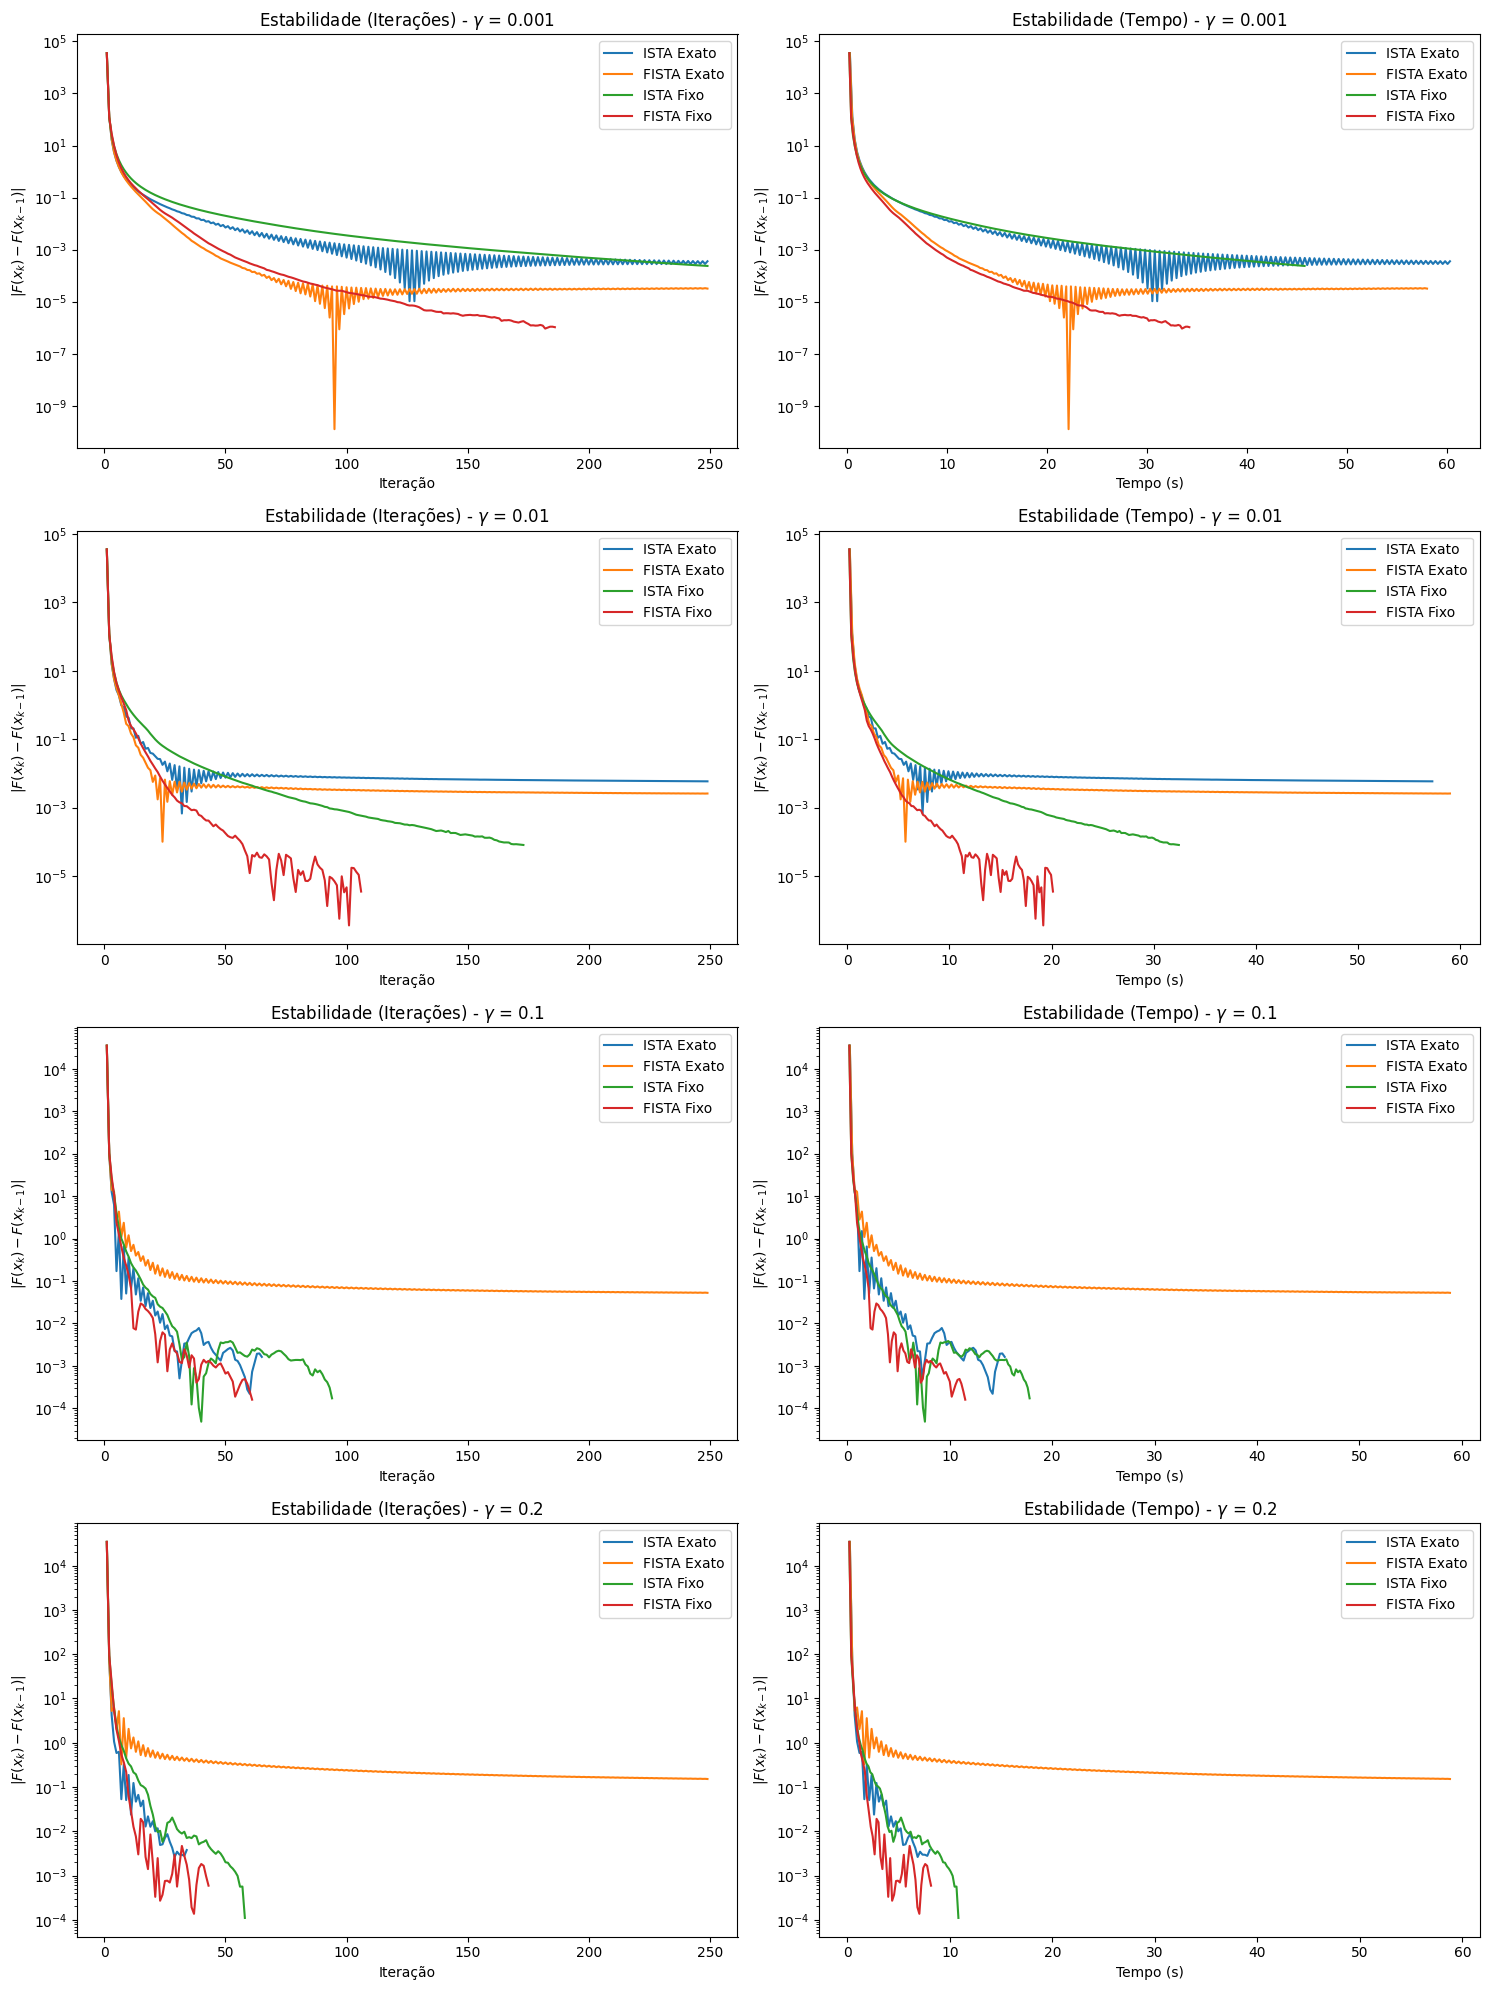
\includegraphics[width=0.8\textwidth]{iterados_gamma_tv.png}
    \caption{Estabilidade iterativa para diferentes valores de $\gamma$ (Variação Total).}
    \label{fig:iterados_gamma_tv}
\end{figure}

\begin{figure}[H]
    \centering
    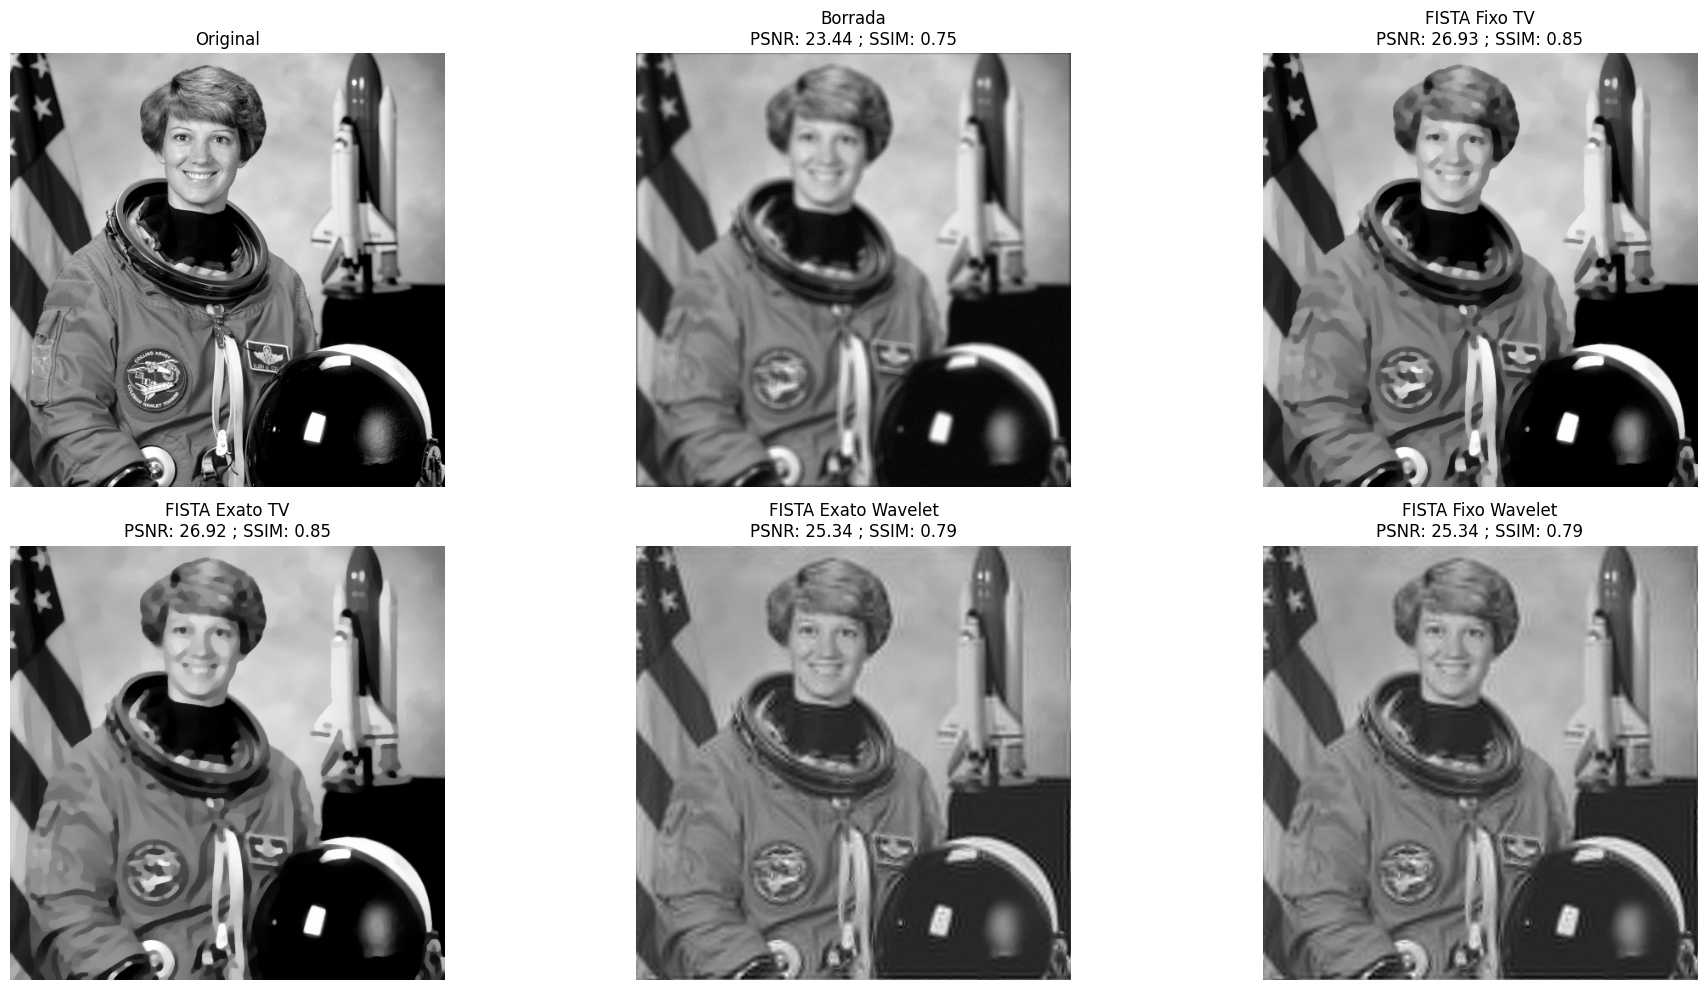
\includegraphics[width=1\textwidth]{comp_wav_tv.png}
    \caption{Qualidade de Reconstrução comparativa: Variação Total \textit{vs.} Wavelet ($\gamma=0.01$, 200 it.).}
    \label{fig:reconst_tv_vs_wav}
\end{figure}

\subsection{Gráficos - Tomografia Computadorizada (Sem Regularização)}

\begin{figure}[H]
    \centering
    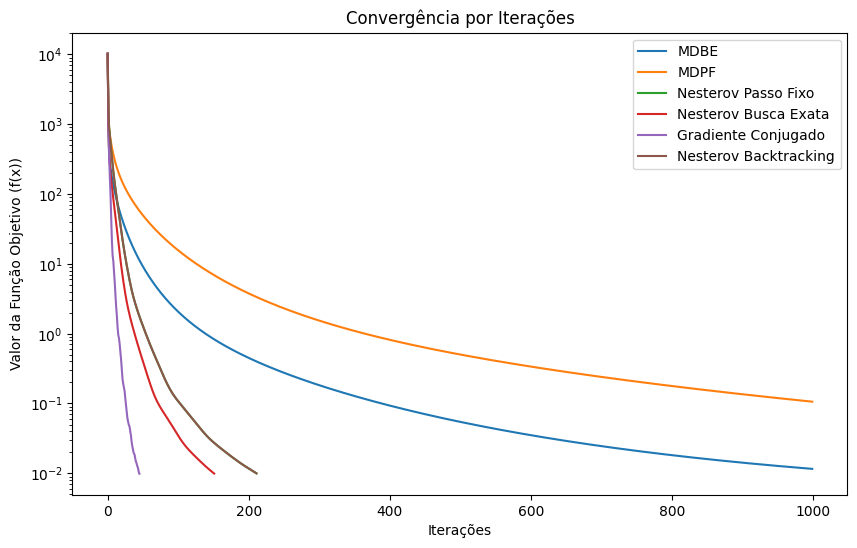
\includegraphics[width=0.8\textwidth]{figuras_sem_reg/conv_iter_exp1.png}
    \caption{Evolução da convergência por número de iterações em TC.}
    \label{fig:tc_sreg_conv_iter1}
\end{figure}

\begin{figure}[H]
    \centering
    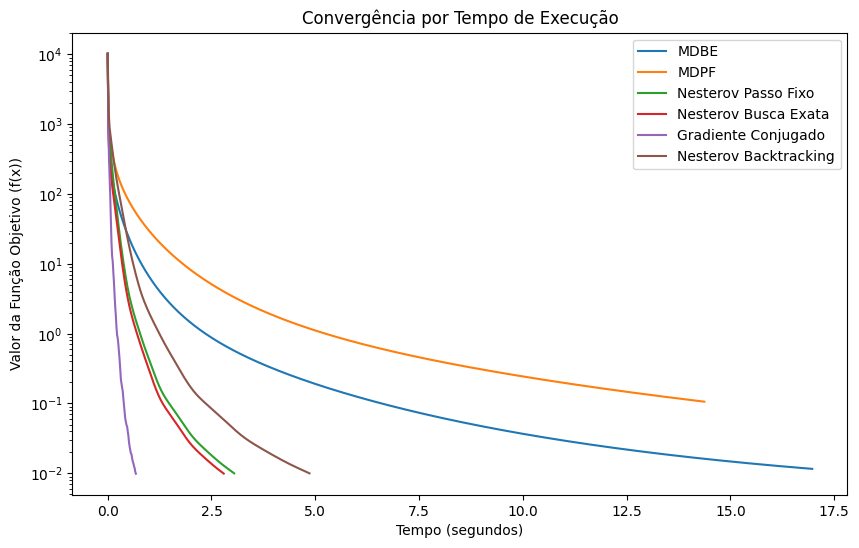
\includegraphics[width=0.8\textwidth]{figuras_sem_reg/conv_temp_exp1.png}
    \caption{Evolução da convergência ao longo do tempo em TC.}
    \label{fig:tc_sreg_conv_temp1}
\end{figure}

\begin{figure}[H]
    \centering
    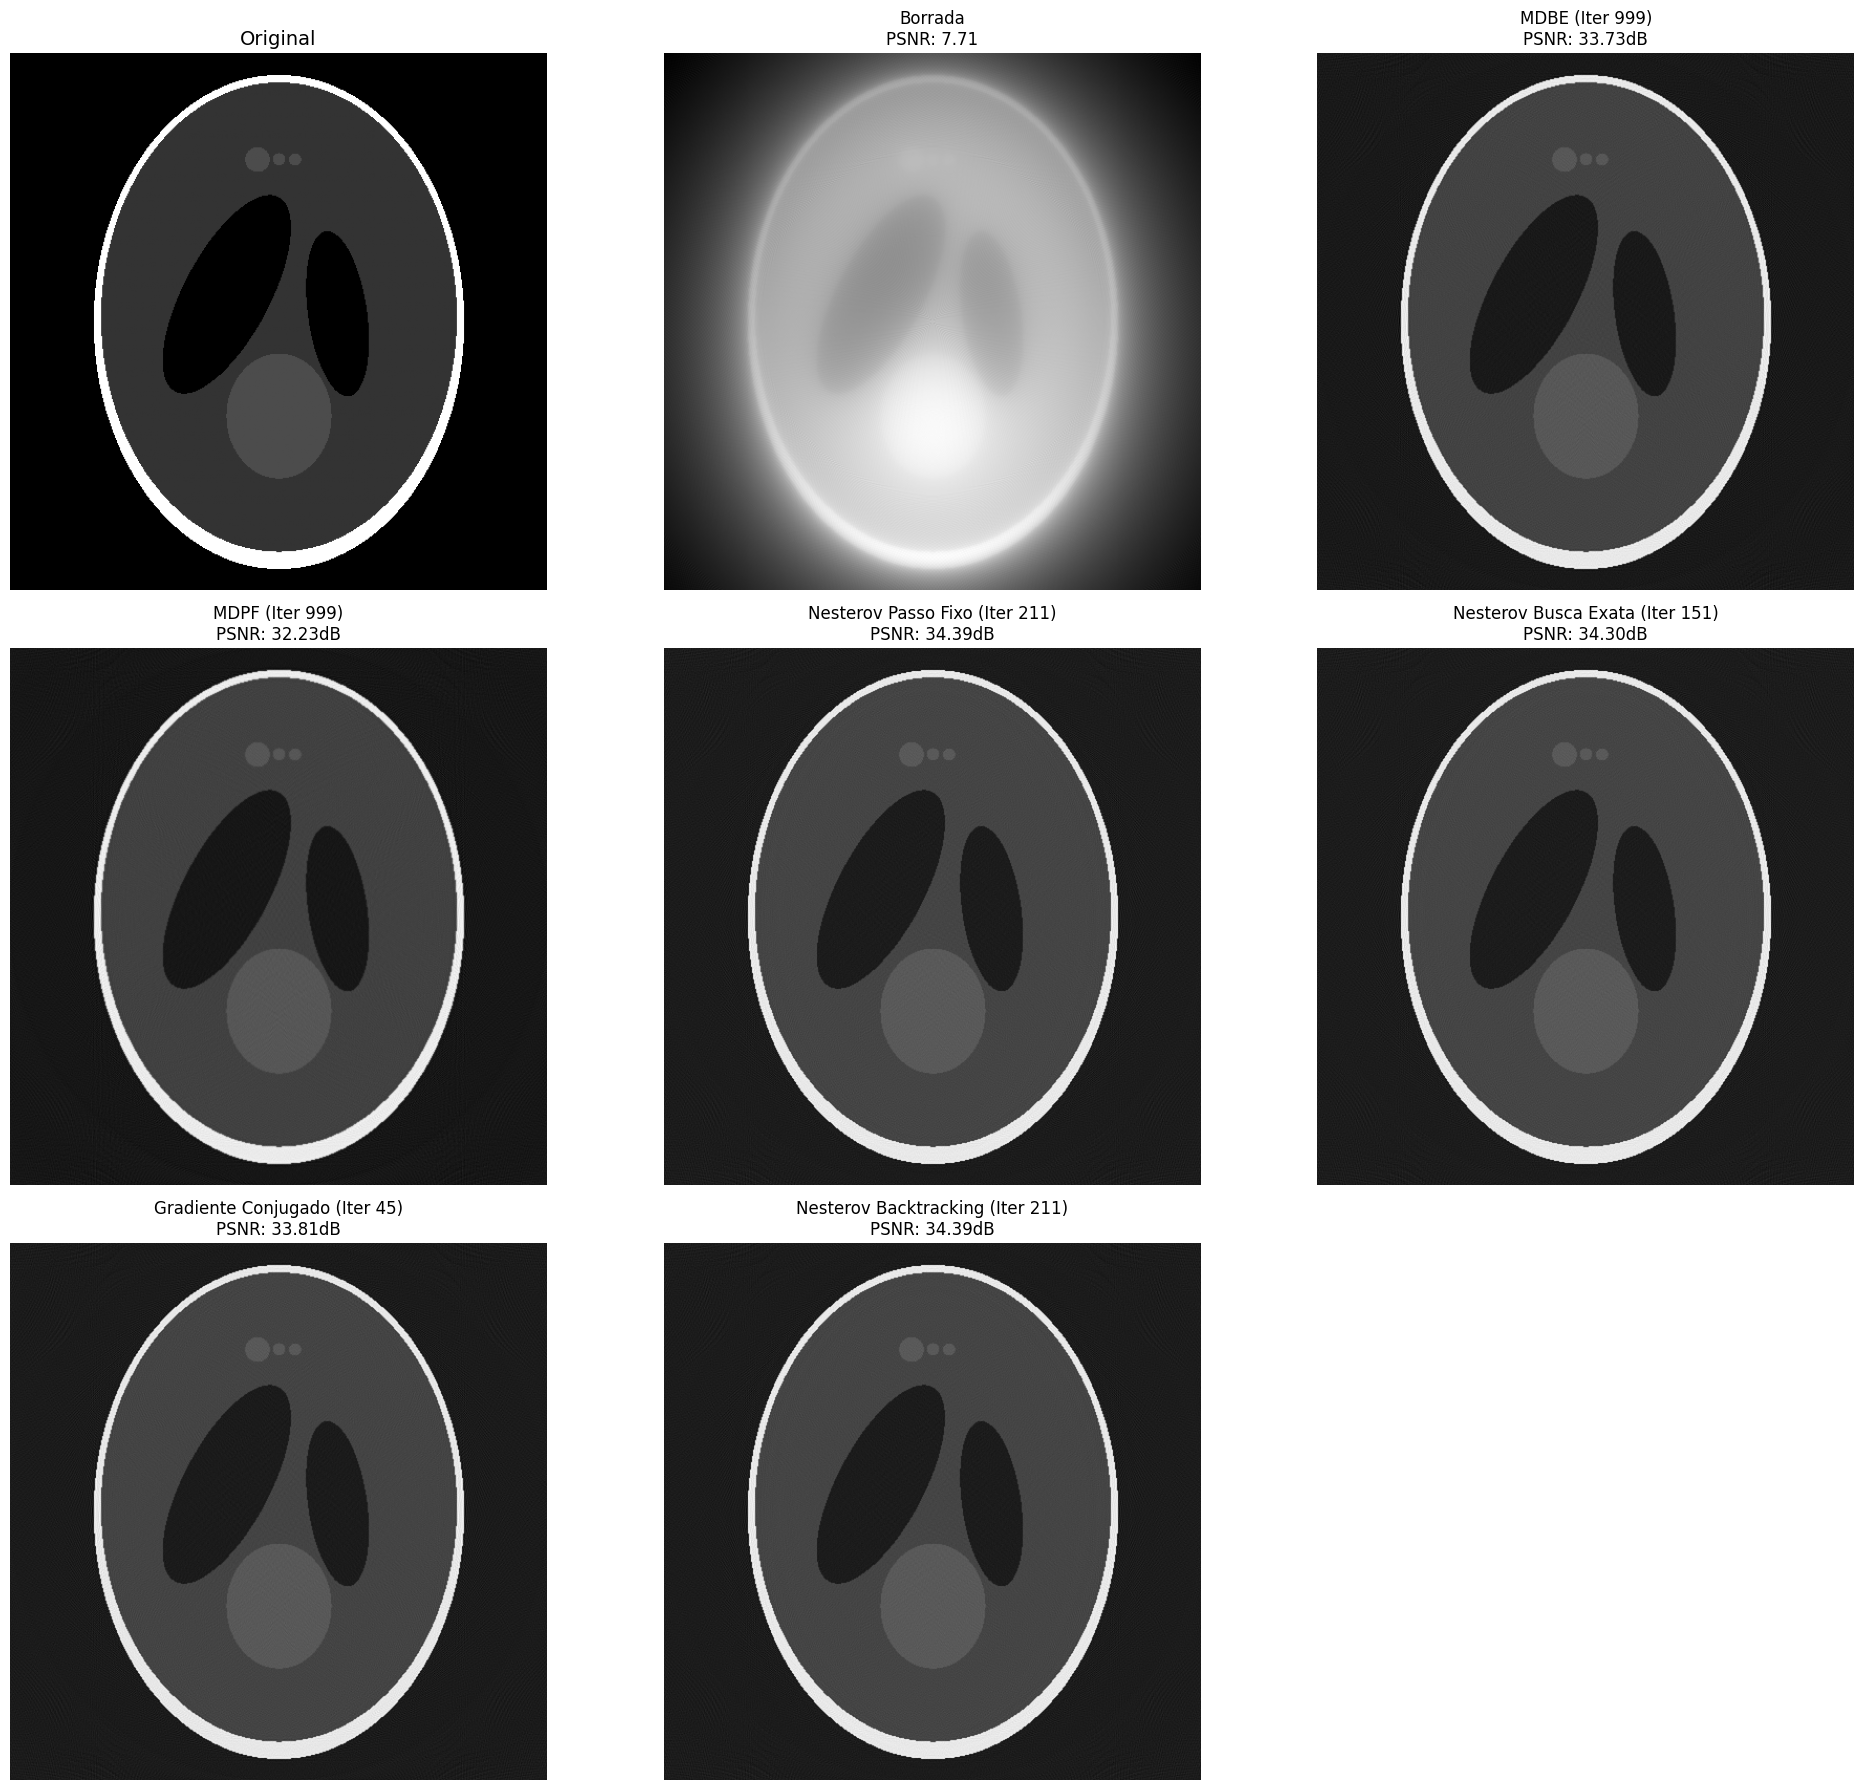
\includegraphics[width=1\textwidth]{figuras_sem_reg/psnr_melhor_img_exp1.png}
    \caption{Reconstruções que atingiram o menor valor de função objetivo para os diferentes métodos.}
    \label{fig:tc_sreg_melhor1}
\end{figure}

\begin{figure}[H]
    \centering
    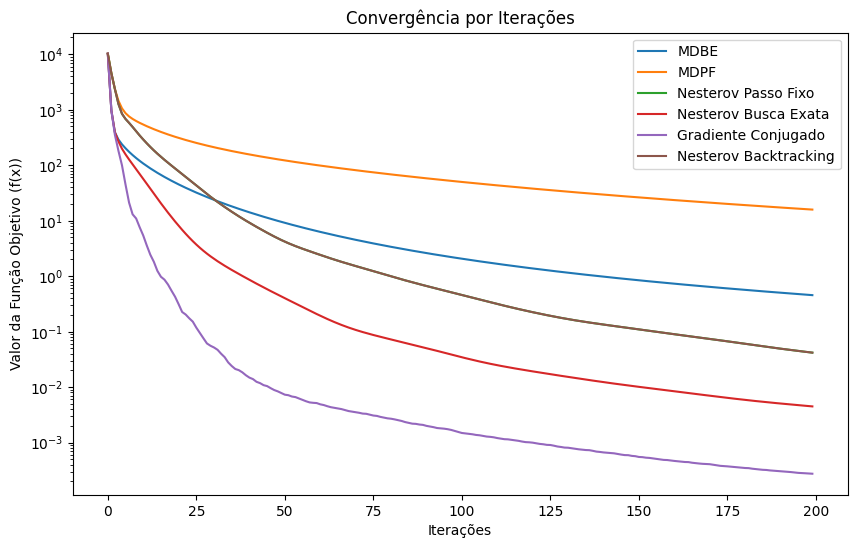
\includegraphics[width=0.9\textwidth]{figuras_sem_reg/conv_iter_exp2.png}
    \caption{Evolução da convergência por iteração para teste com 200 iterações.}
    \label{fig:tc_sreg_conv_iter2}
\end{figure}

\begin{figure}[H]
    \centering
    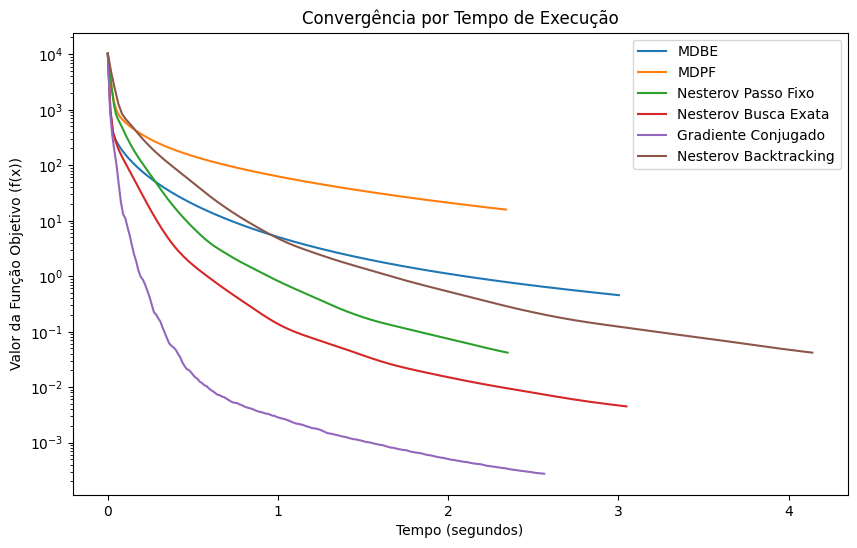
\includegraphics[width=0.9\textwidth]{figuras_sem_reg/conv_temp_exp2.png}
    \caption{Evolução da convergência ao longo do tempo para teste com 200 iterações.}
    \label{fig:tc_sreg_conv_temp2}
\end{figure}

\begin{figure}[H]
    \centering
    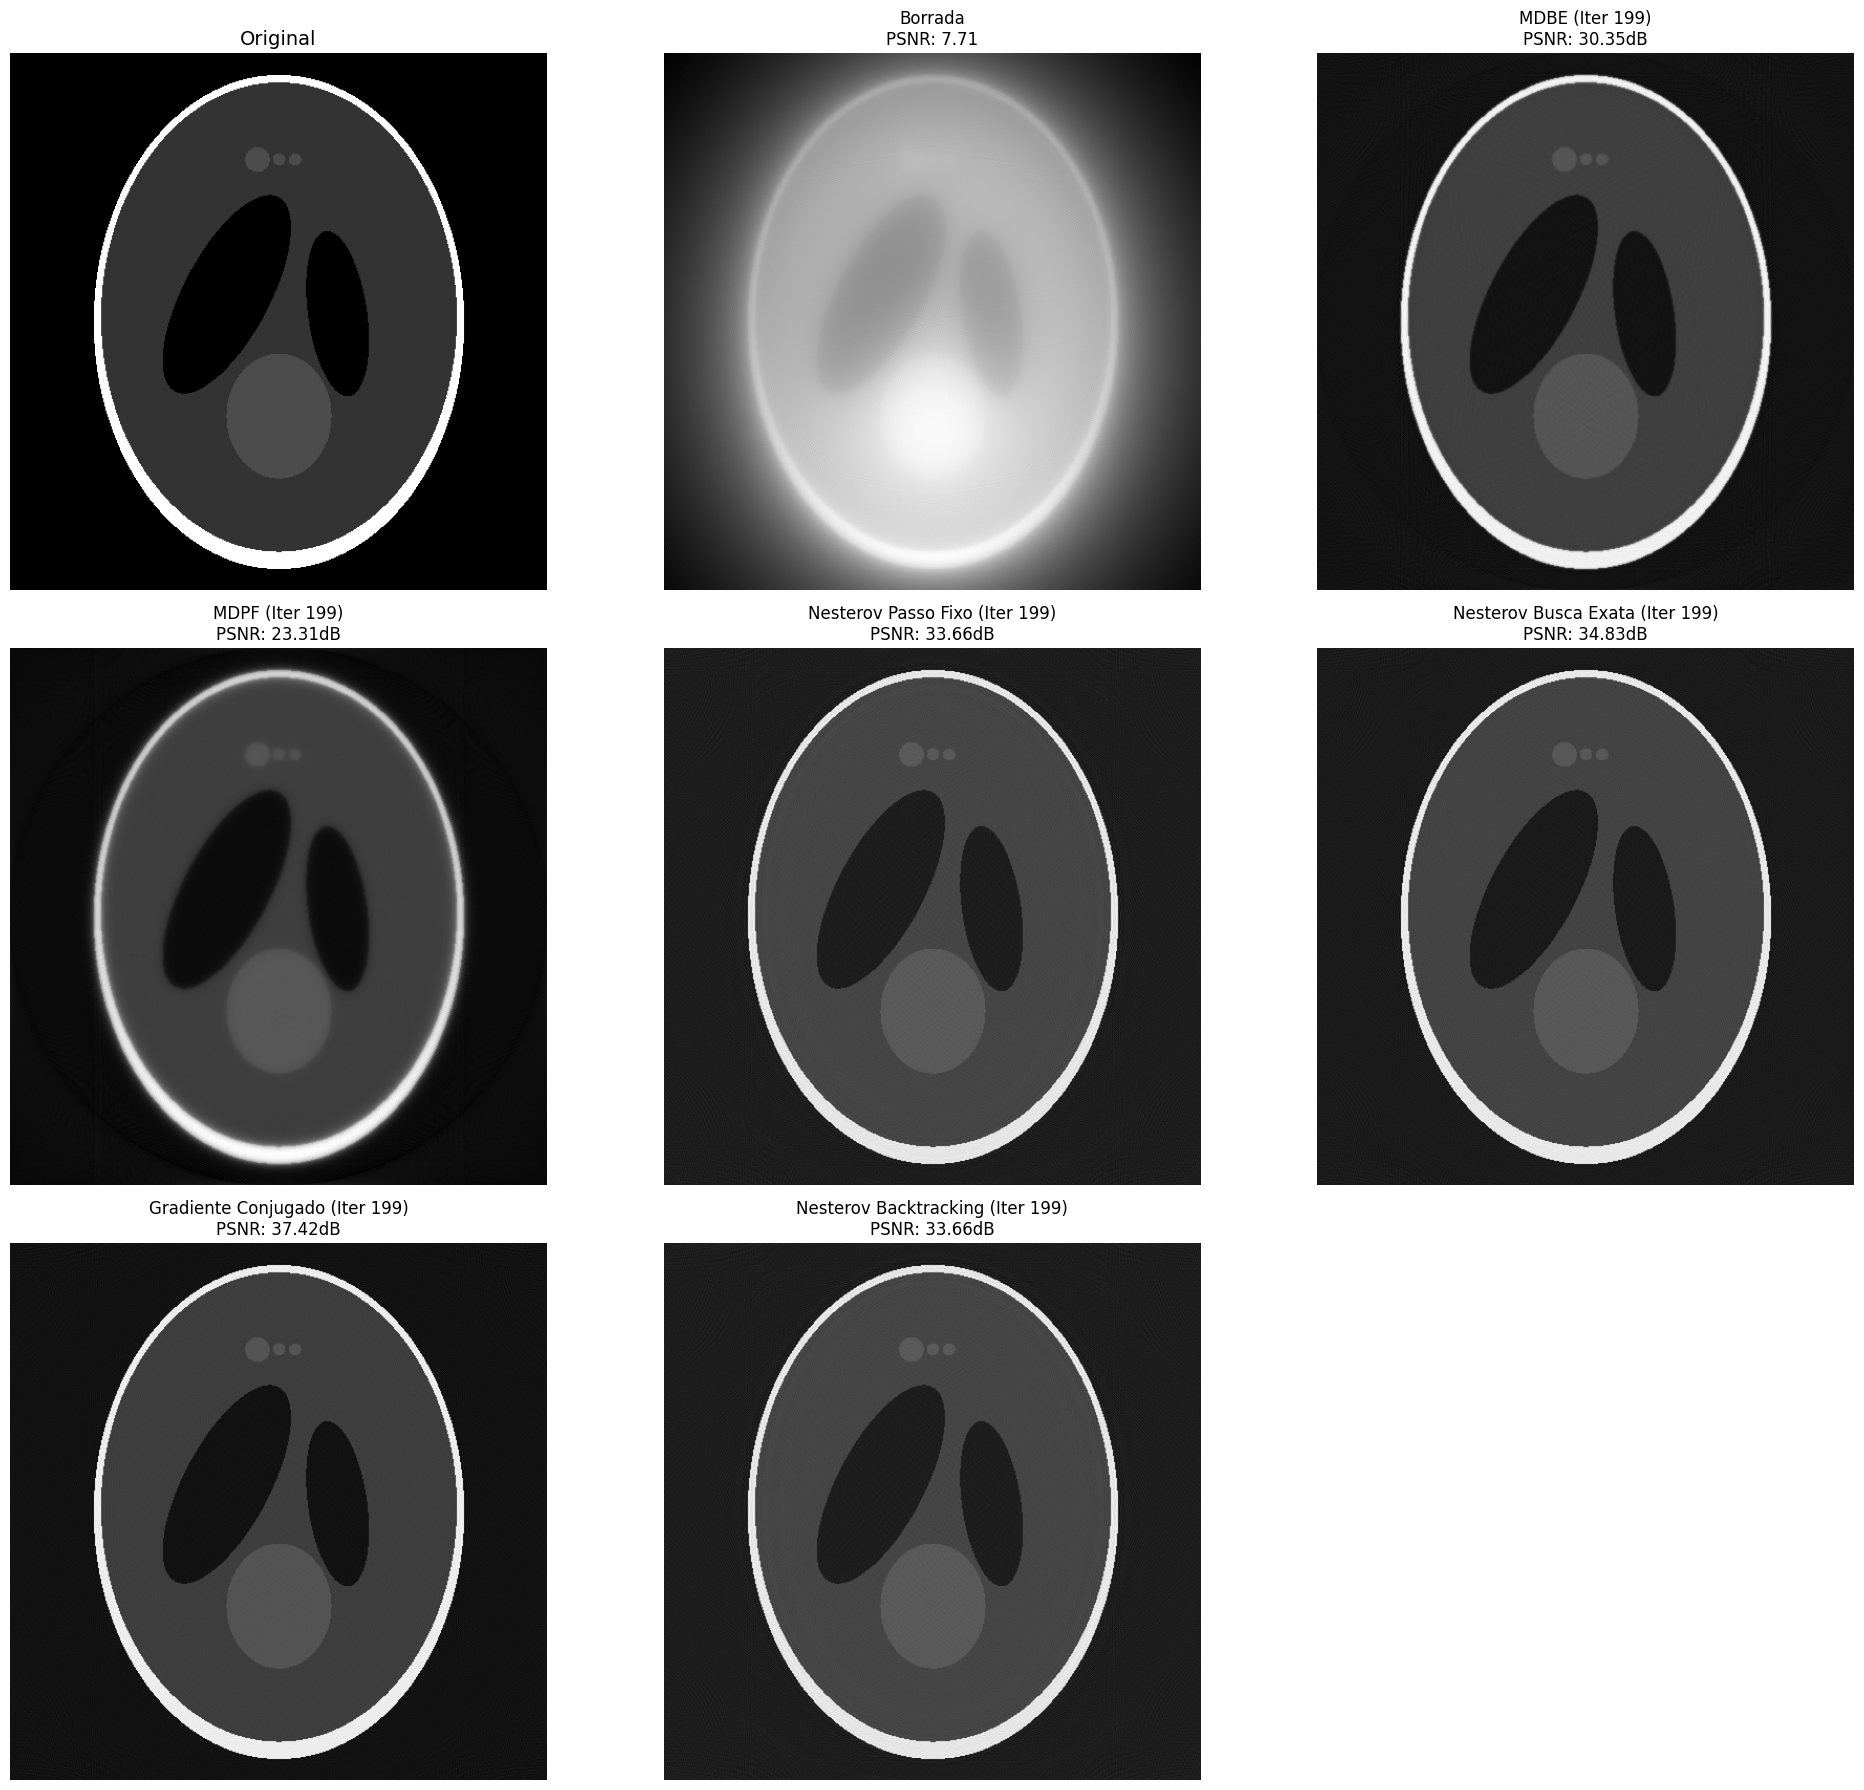
\includegraphics[width=1\textwidth]{figuras_sem_reg/melhor_psnr_exp2.png}
    \caption{Melhores reconstruções (que atingiram o menor valor de função objetivo) obtidas no teste com 200 iterações.}
    \label{fig:tc_sreg_melhor2}
\end{figure}

\begin{figure}[H]
    \centering
    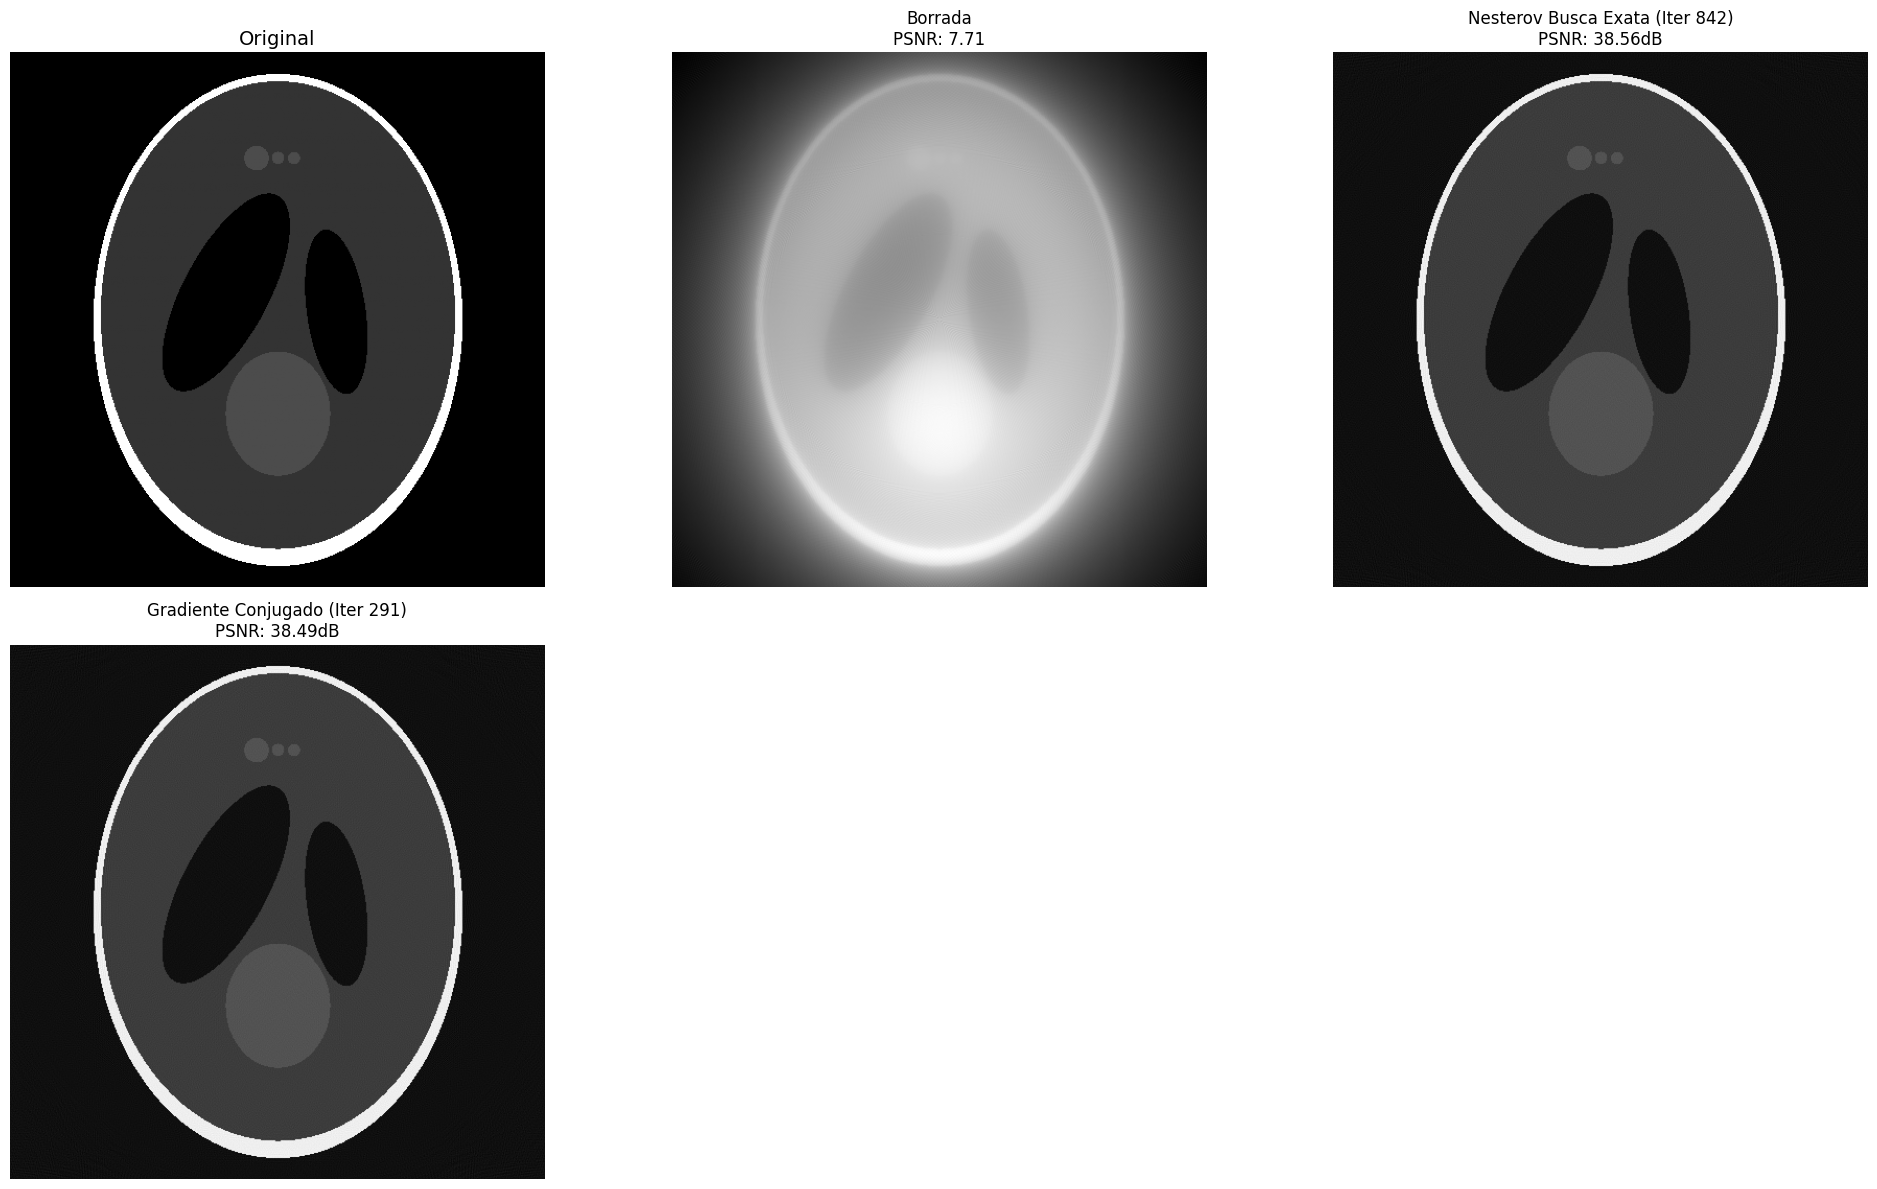
\includegraphics[width=1\textwidth]{figuras_sem_reg/imgs_psnr_buscaexata_conjugado1.png}
    \caption{Comparação visual: Nesterov Busca Exata \textit{vs} Gradientes Conjugados com tolerância de $10^{-4}$.}
    \label{fig:tc_sreg_nest_gc1}
\end{figure}

\begin{figure}[H]
    \centering
    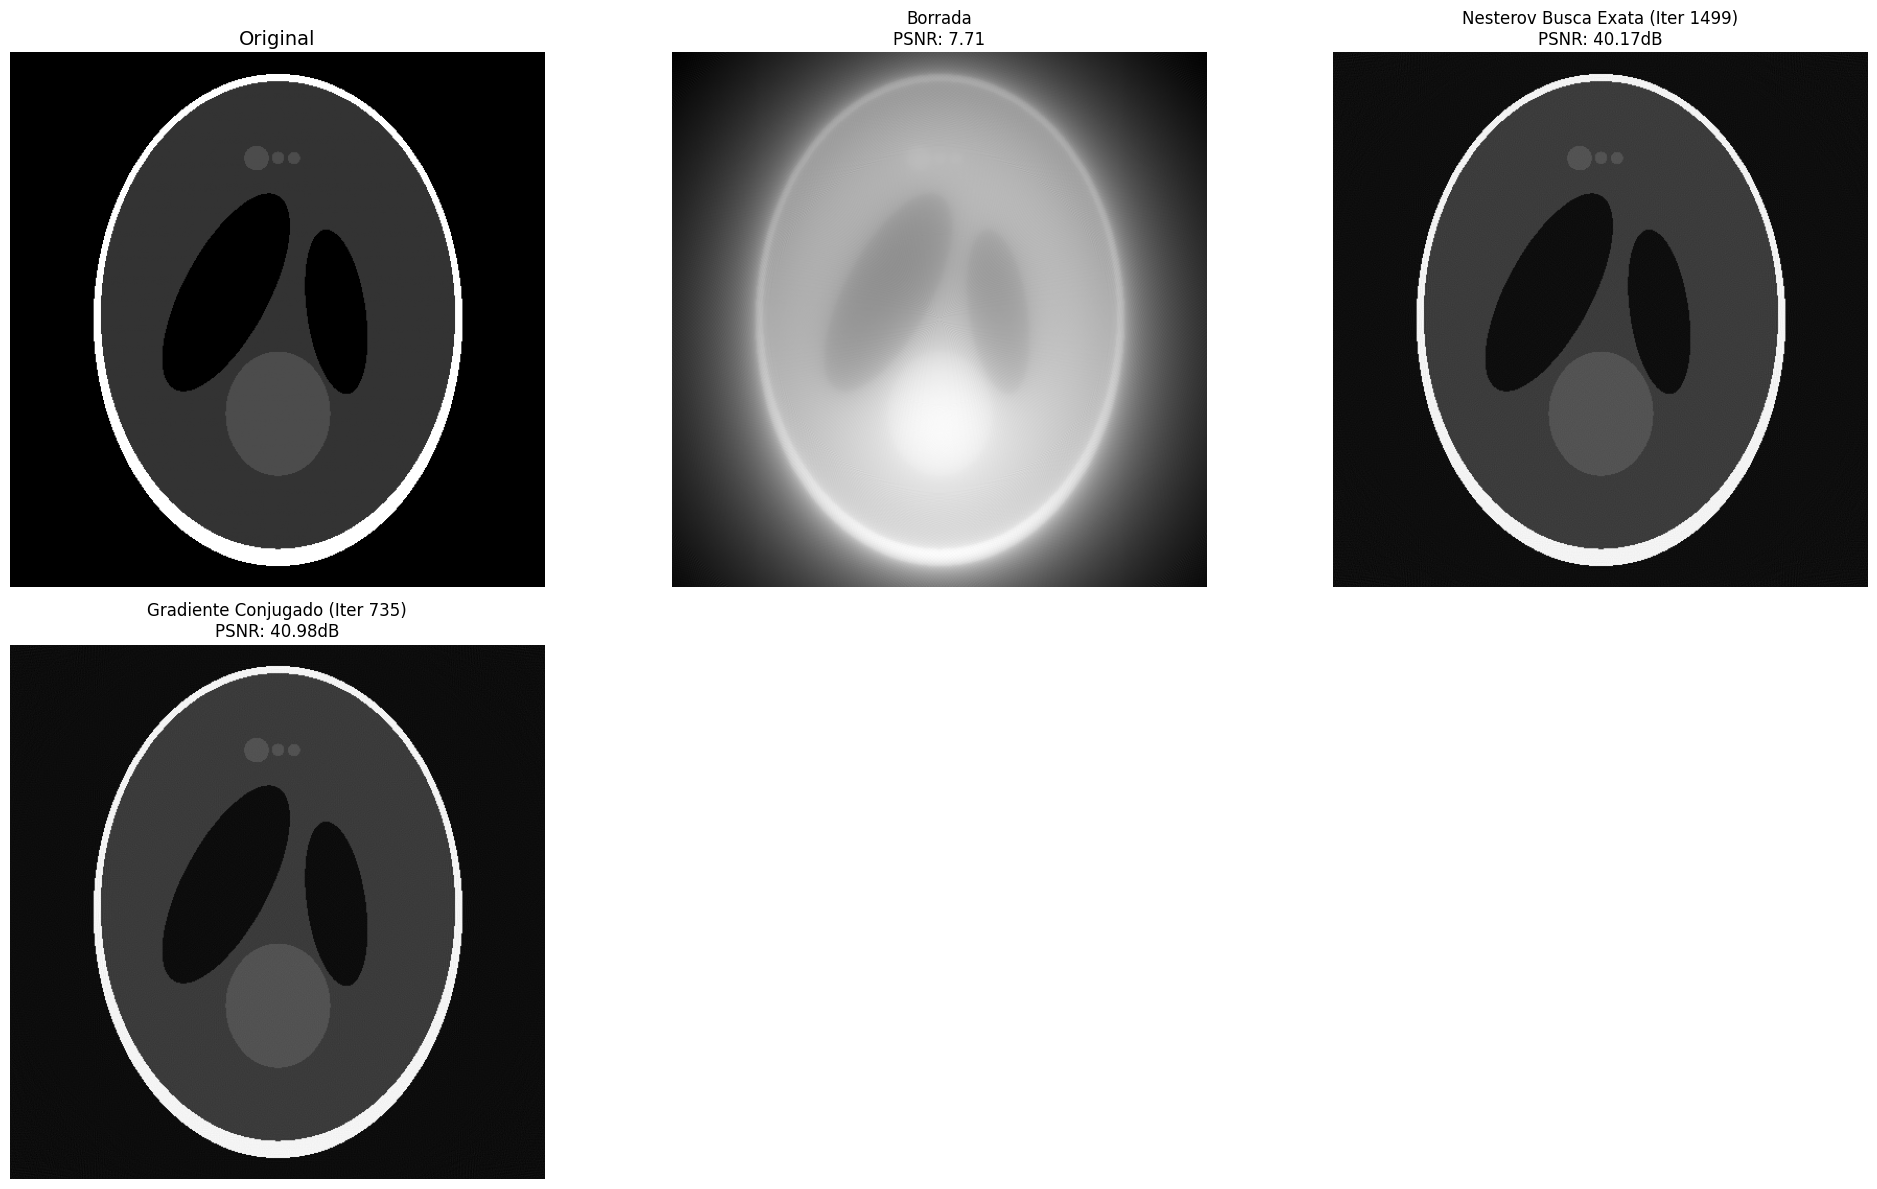
\includegraphics[width=1\textwidth]{figuras_sem_reg/imgs_psnr_buscaexata_conjugado_exp2.png}
    \caption{Comparação visual: Nesterov Busca Exata \textit{vs} Gradientes Conjugados com tolerância de $10^{-5}$.}
    \label{fig:tc_sreg_nest_gc2}
\end{figure}
    
\subsection{Gráficos - Tomografia Computadorizada (\textit{Wavelets} e Variação Total)}

\begin{figure}[H]
    \centering
    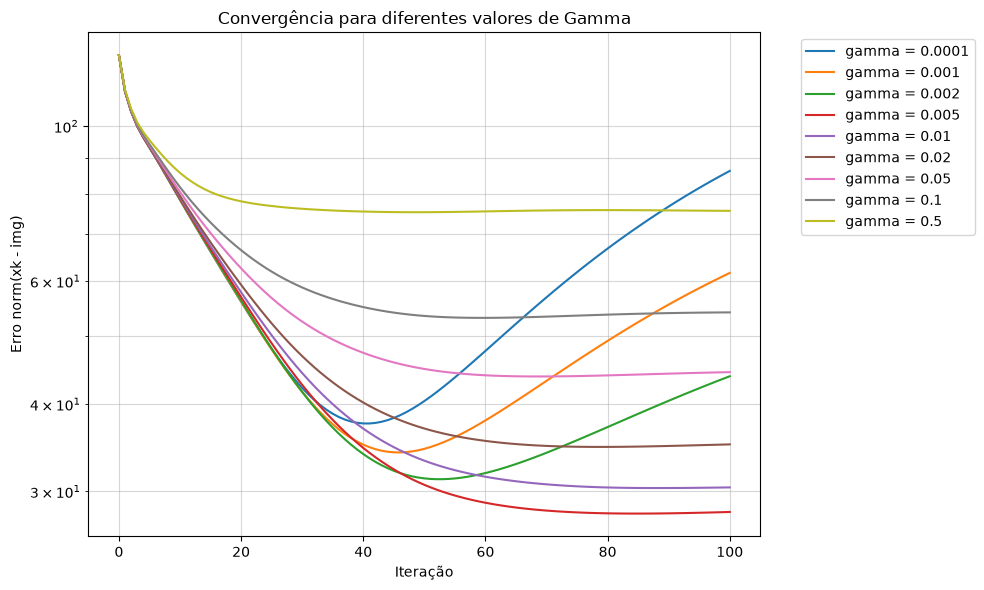
\includegraphics[width=0.9\textwidth]{figuras_wav/grid_gamma.png}
    \caption{\textit{Grid-Search} para determinação do parâmetro de regularização $\gamma=0.005$ em TC com \textit{Wavelets}.}
    \label{fig:tc_wav_grid}
\end{figure}

\begin{figure}[H]
    \centering
    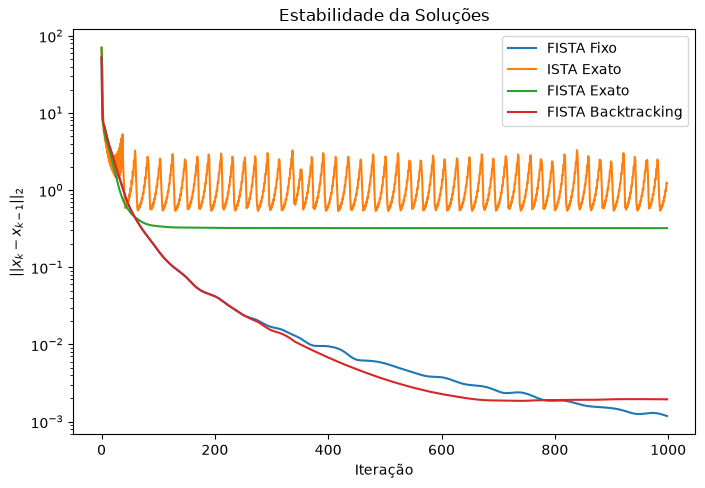
\includegraphics[width=0.8\textwidth]{figuras_wav/diff_iterados.png}
    \caption{Diferença $\norm{\mathbf{x_k} - \mathbf{x_{k-1}}}$ em TC com \textit{Wavelets}.}
    \label{fig:tc_norm_diff}
\end{figure}

\begin{figure}[H]
    \centering
    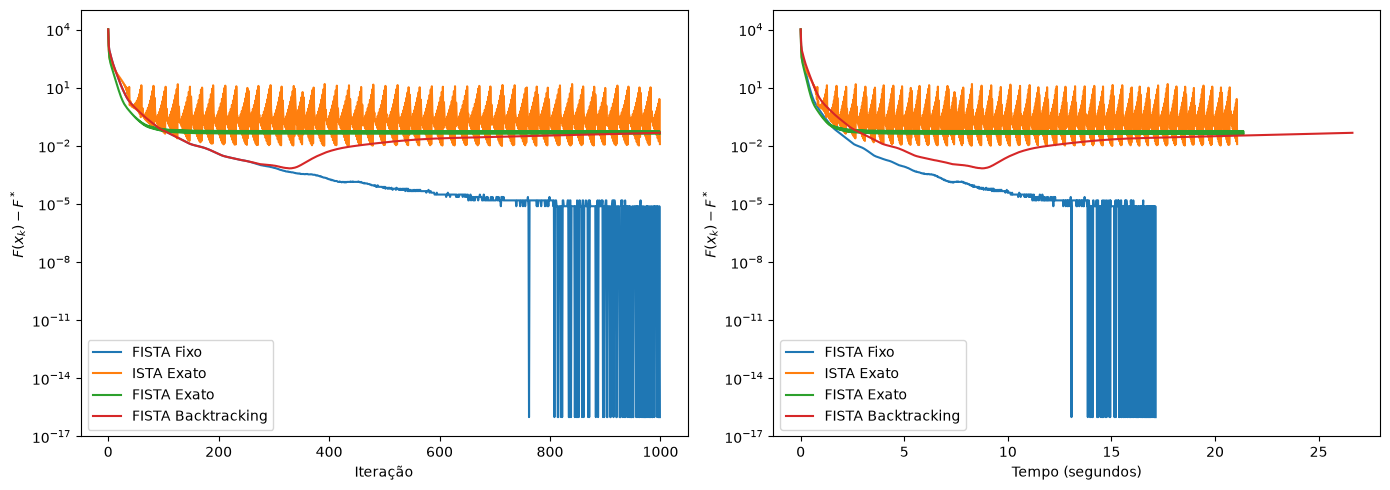
\includegraphics[width=1\textwidth]{figuras_wav/diff_valor_funcao_otimo_temp_e_iter.png}
    \caption{Evolução de $F(\mathbf{x}_k) - F^*$ em TC com \textit{Wavelets}, demonstrando a instabilidade assintótica.}
    \label{fig:tc_wav_diff_func}
\end{figure}

\begin{figure}[H]
    \centering
    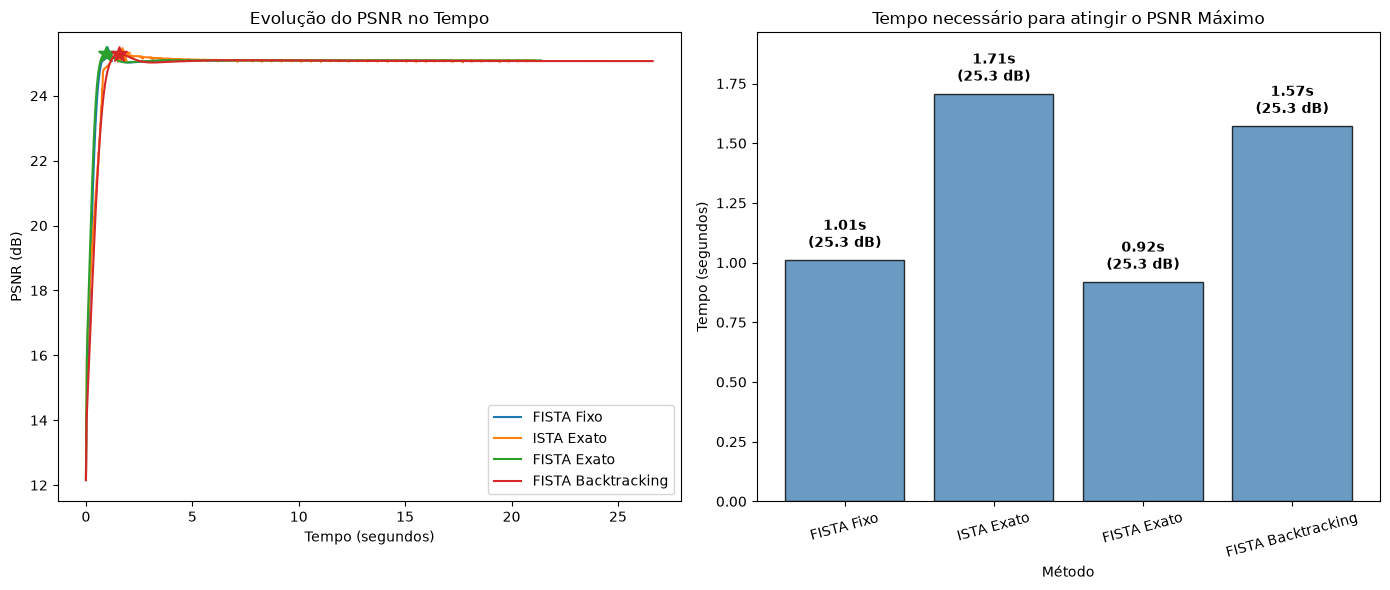
\includegraphics[width=1\textwidth]{figuras_wav/evolucao_psnr_e_tempo_psnr_max.png}
    \caption{Evolução do PSNR em TC com \textit{Wavelets}.}
    \label{fig:tc_psnr}
\end{figure}

\begin{figure}[H]
    \centering
    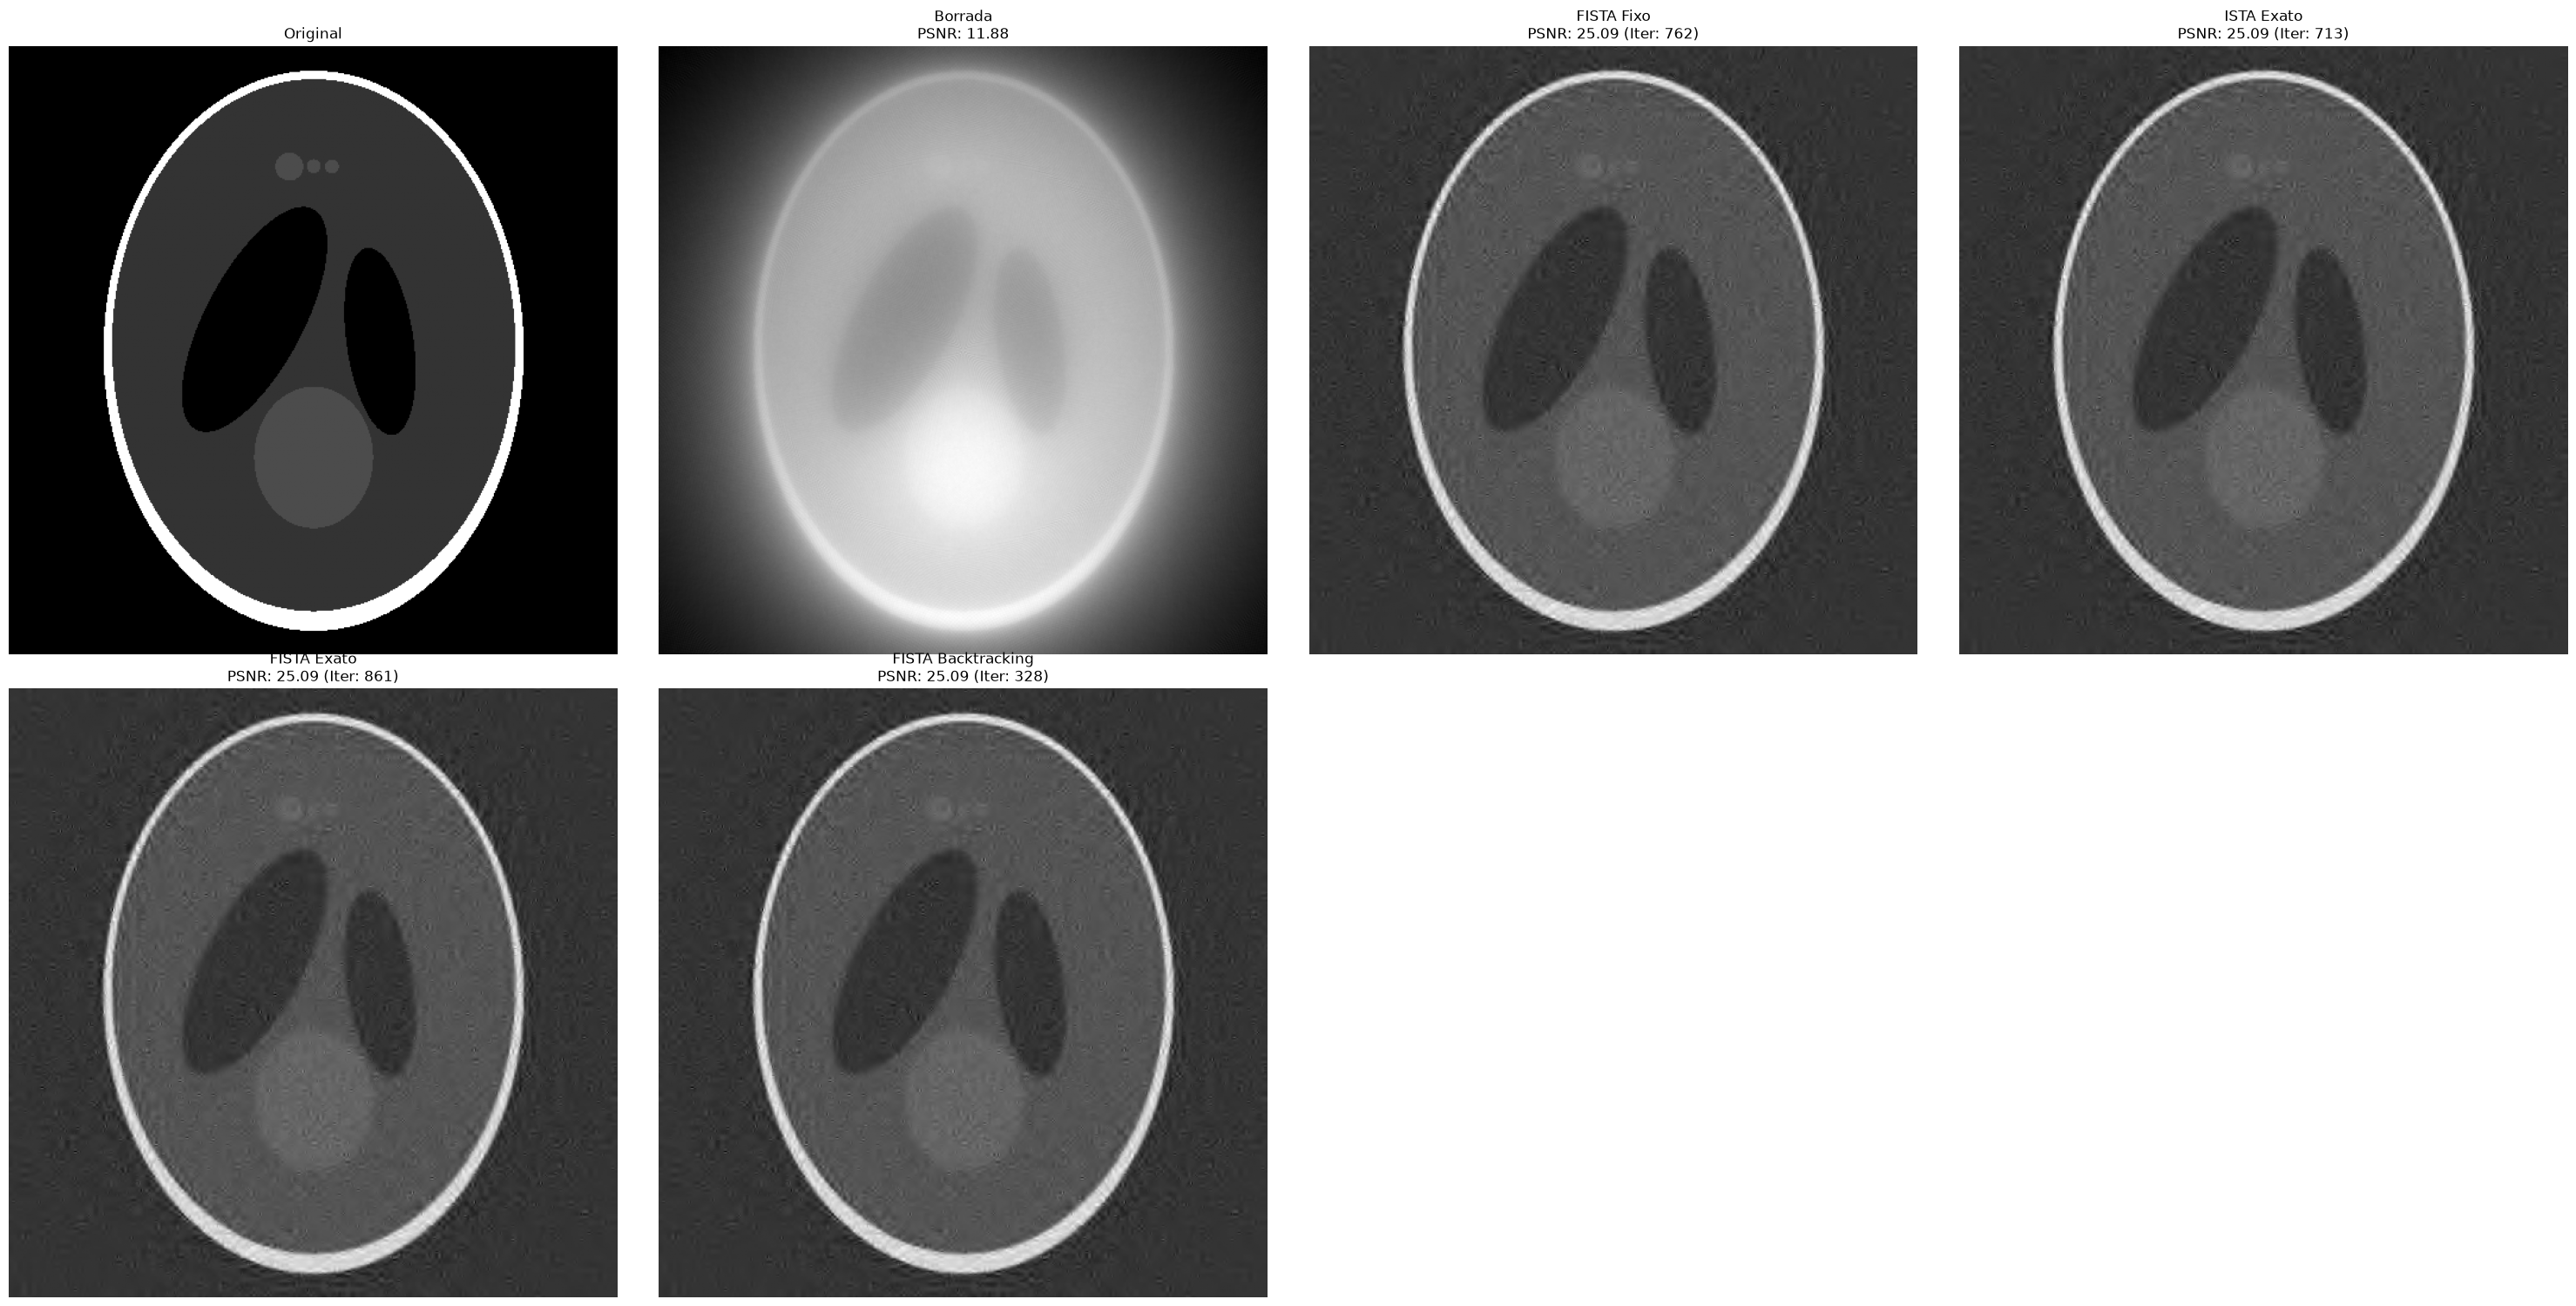
\includegraphics[width=1\textwidth]{figuras_wav/melhores_reconstrucoes.png}
    \caption{Melhores reconstruções obtidas (que minimizam a função objetivo) e qualidade visual em TC com \textit{Wavelets}.}
    \label{fig:tc_wav_reconst}
\end{figure}

\begin{figure}[H]
    \centering
    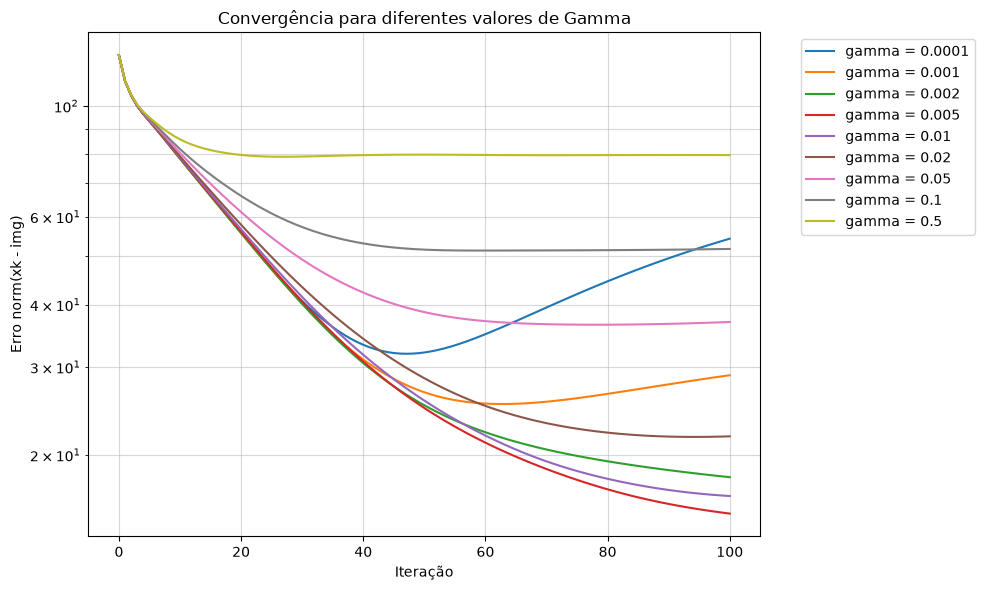
\includegraphics[width=0.9\textwidth]{figuras_tv/grid_search.png}
    \caption{\textit{Grid-Search} para determinação do parâmetro de regularização $\gamma=0.005$ em TC com Variação Total.}
    \label{fig:grid_search_tv}
\end{figure}

\begin{figure}[H]
    \centering
    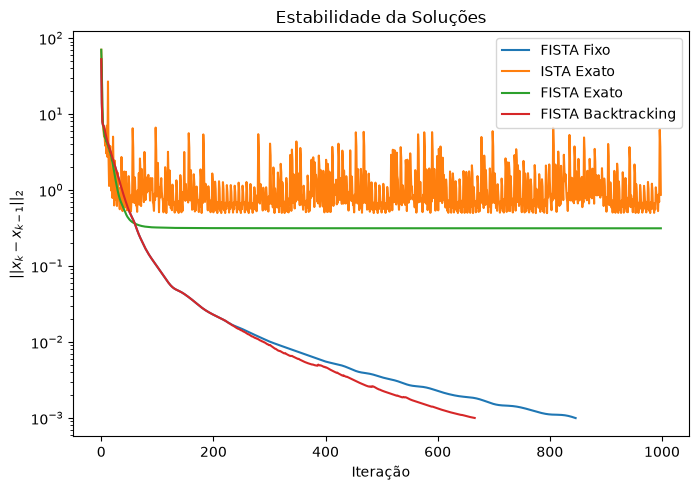
\includegraphics[width=0.8\textwidth]{figuras_tv/diff_iters_estabilidade.png}
    \caption{Diferença $\norm{\mathbf{x_k} - \mathbf{x_{k-1}}}$ em TC com Variação Total}
    \label{fig:tc_tv_diff_iter}
\end{figure}

\begin{figure}[H]
    \centering
    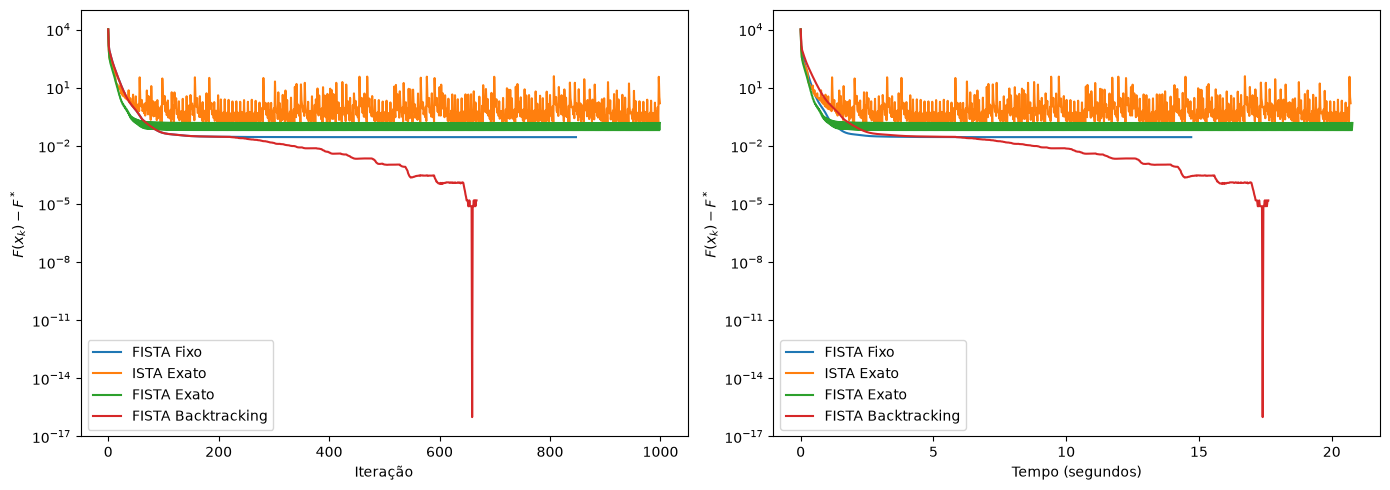
\includegraphics[width=1\textwidth]{figuras_tv/fxk_fstar_tempo_e_iter.png}
    \caption{Evolução de $F(\mathbf{x}_k) - F^*$ em TC com Variação Total, ilustrando a instabilidade assintótica no ISTA Exato e FISTA Exato em comparação com FISTA Fixo.}
    \label{fig:tc_tv_diff_func}
\end{figure}

\begin{figure}[H]
    \centering
    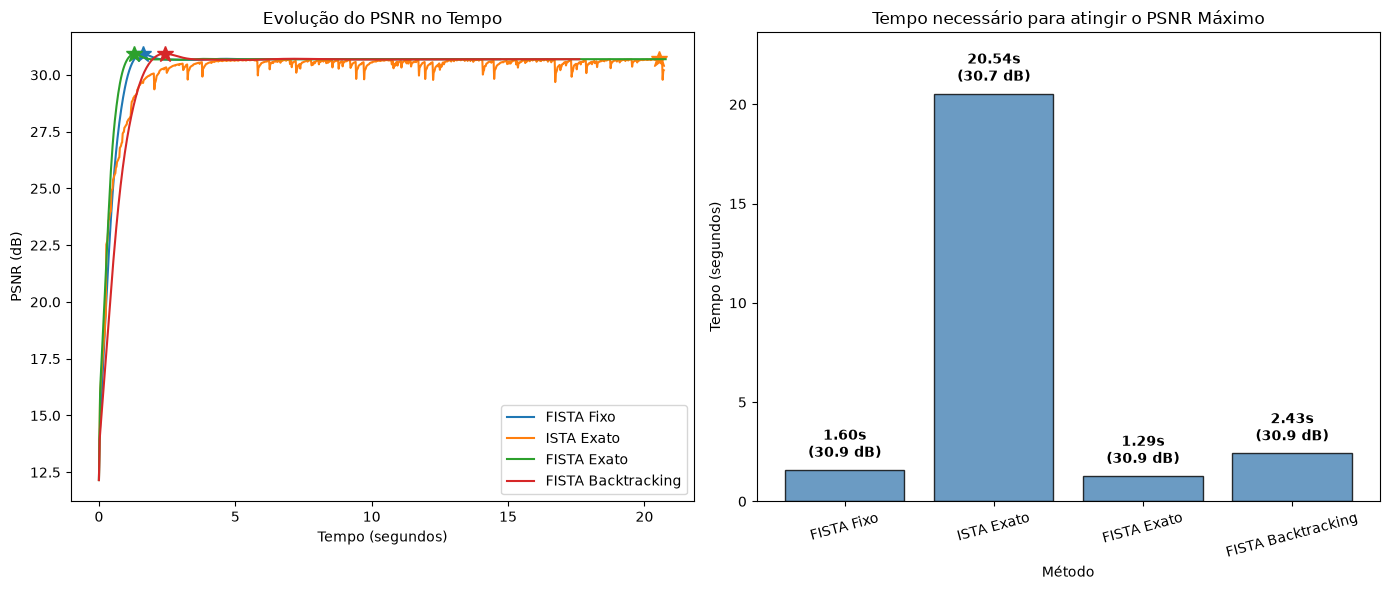
\includegraphics[width=1\textwidth]{figuras_tv/evolucao_psnr.png}
    \caption{Evolução do PSNR em TC com Variação Total.}
    \label{fig:tc_tv_psnr}
\end{figure}

\begin{figure}[H]
    \centering
    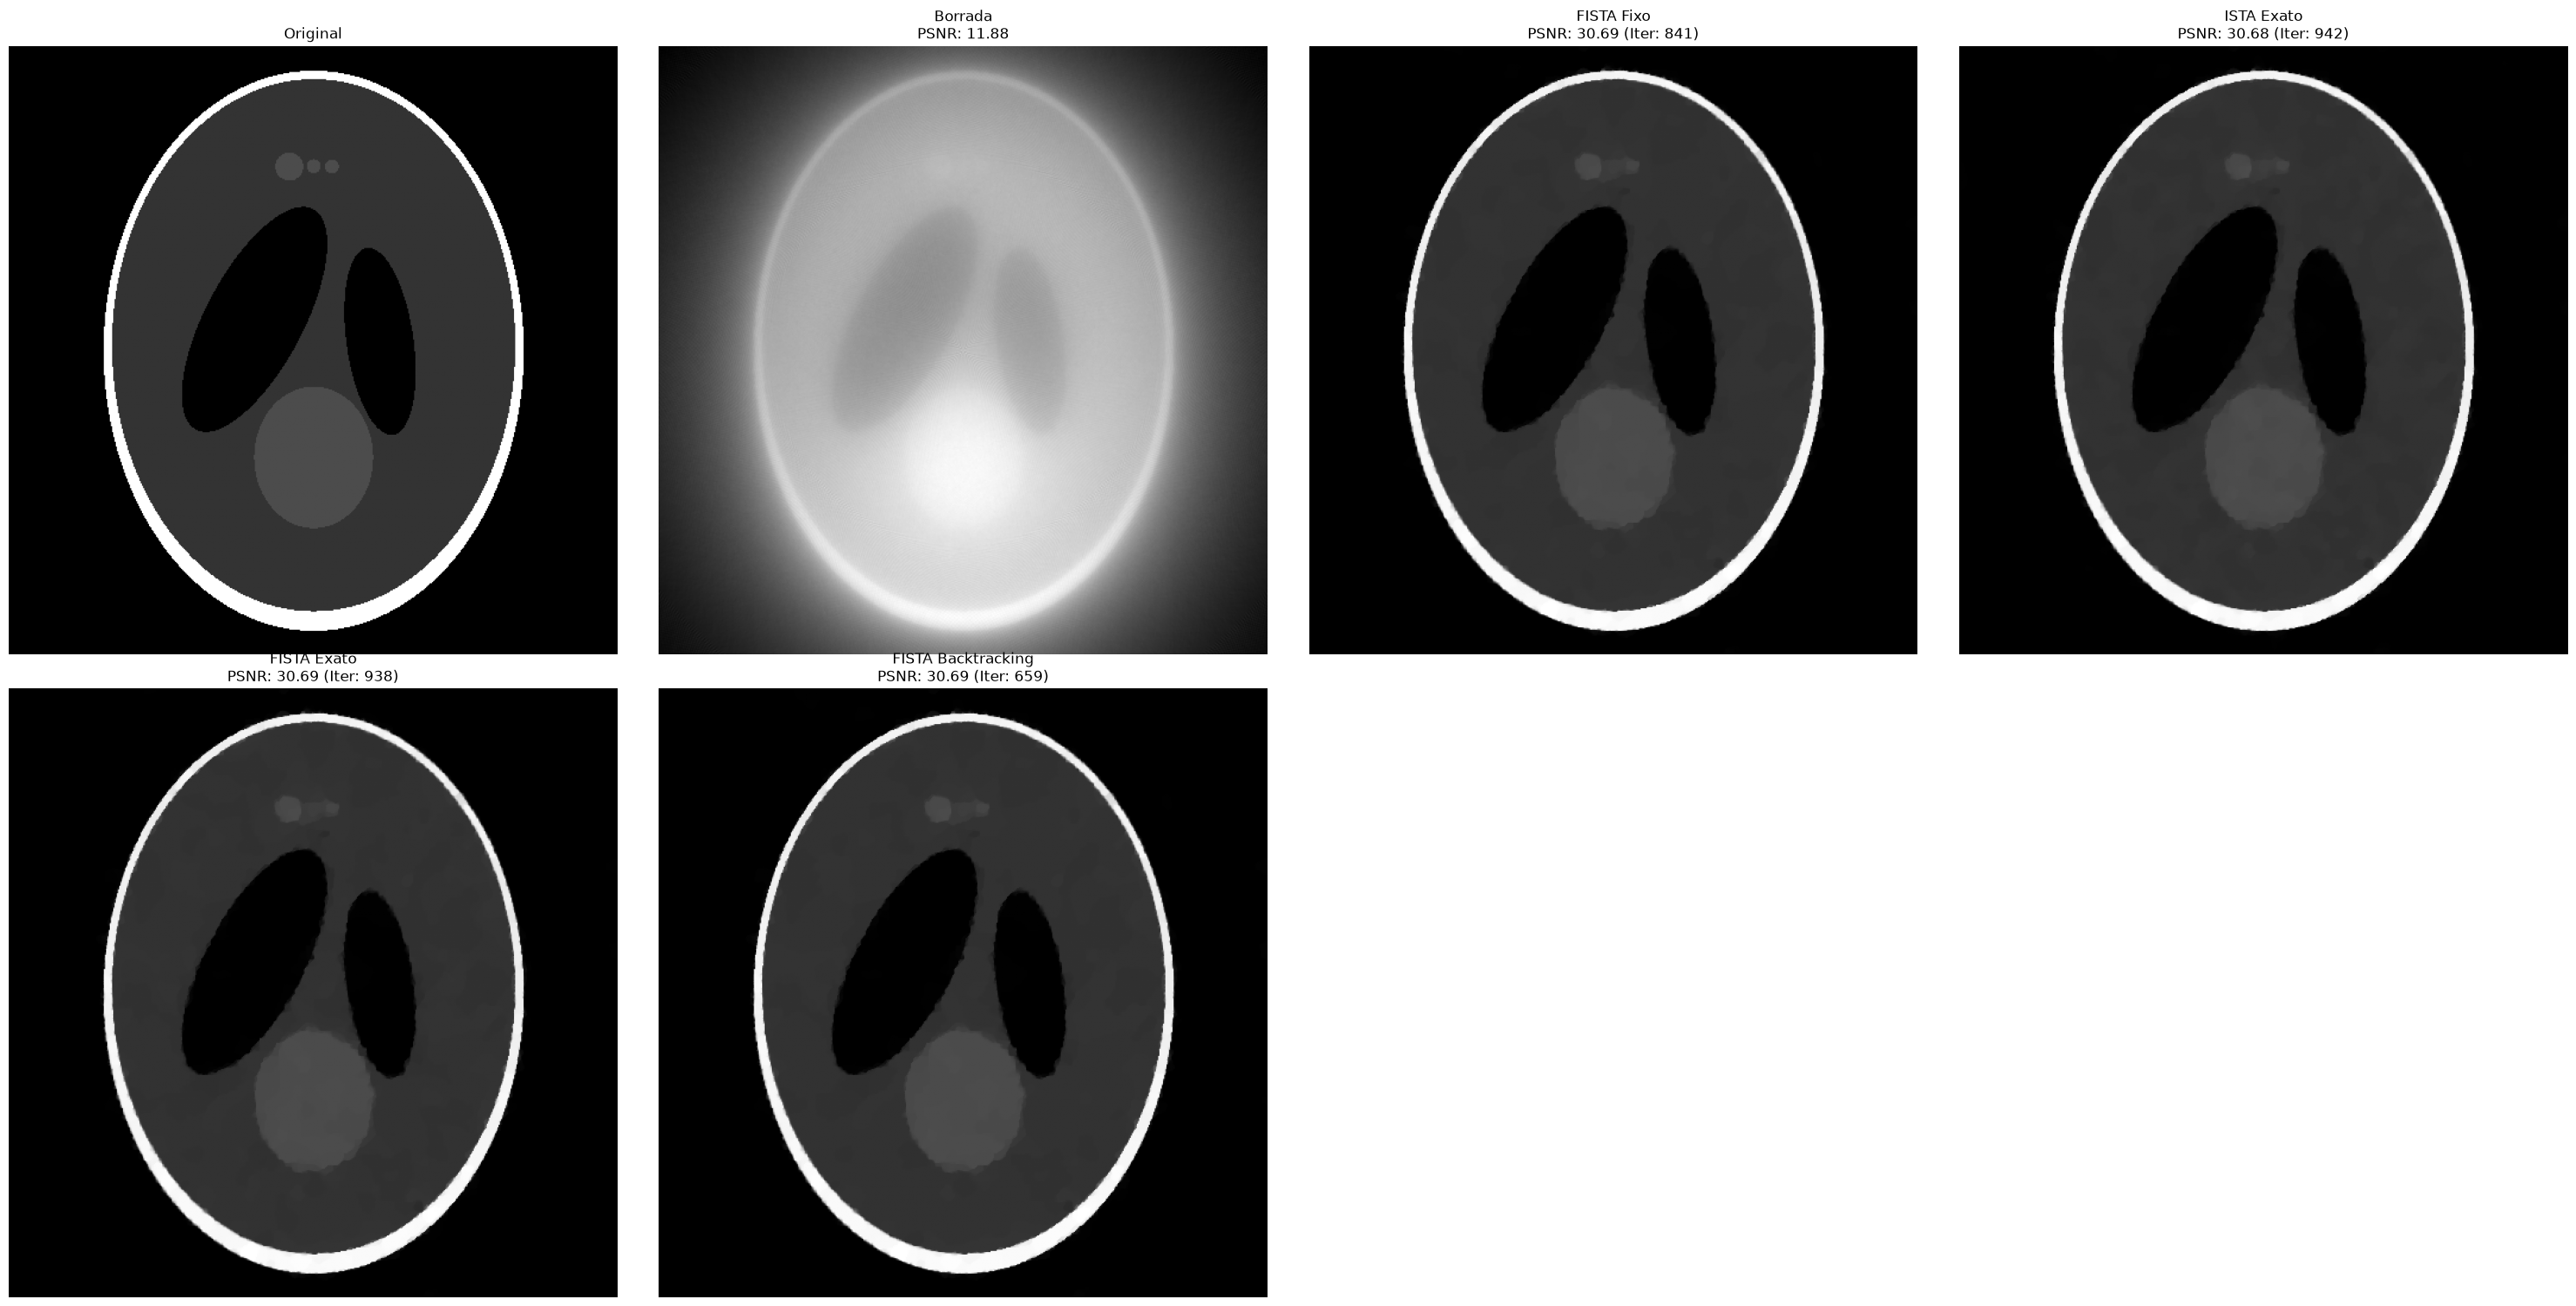
\includegraphics[width=1\textwidth]{figuras_tv/melhores_reconstrucoes_minimizando_func.png}
    \caption{Melhores reconstruções obtidas (que minimizam a função objetivo) e qualidade visual em TC com Variação Total.}
    \label{fig:tc_tv_reconst}
\end{figure}

\end{document} 